\documentclass{beamer}
\usetheme{Madrid}
\usecolortheme{default}
\usepackage{xcolor}

\definecolor{color1}{HTML}{B8B8B8} % Lighter version of dark gray
\definecolor{color2}{HTML}{A8C4C6} % Lighter version of teal
\definecolor{color3}{HTML}{7FA6D1} % Lighter version of blue
\definecolor{color4}{HTML}{F2C199} % Lighter version of orange
\definecolor{color5}{HTML}{D08080} % Lighter version of maroon
\definecolor{color6}{HTML}{80C080} % Lighter version of green
\definecolor{lightblue}{RGB}{173,216,230} % Light blue color
\definecolor{darkblue}{RGB}{0,0,139} % Dark blue color

% Package imports
\usepackage{graphicx}
\usepackage{booktabs}
\usepackage{graphicx} % Required for inserting images
\usepackage{rotating} % Required for sidewaysfigure
\usepackage{adjustbox} % To adjust regression tables
\usepackage{lscape} % To activate landscape mode
\usepackage{subcaption} % To use subfigures
\usepackage{tikz} % To draw figures
\usetikzlibrary{positioning}
\usepackage{xcolor} % To define custom colors
\usepackage{bbm} % To use indicator function
\usepackage{amsmath} % To use math symbols
\usepackage{hyperref}

\usepackage[authordate,backend=biber,maxnames=3,minnames=1, dashed=false, maxbibnames =99]{biblatex-chicago} % Use the Chicago author-date style
\addbibresource{references.bib}
% Customize the citation format to put the year in parentheses
\renewbibmacro*{cite:labelyear+extrayear}{%
  \iffieldundef{labelyear}
    {}
    {\printtext[bibhyperref]{%
       \mkbibparens{\printfield{labelyear}%
       \printfield{extrayear}}}}}

% Title page information
\title{Europe's Digitalization and the EDIH initiative: \\What leads firms to participate?}
\author{Federico Vicentini}
\institute{Università Cattolica del Sacro Cuore\\
Department of Economics}
\date{April 10, 2025}
\setbeamertemplate{navigation symbols}{}
\setbeamertemplate{footline}{}
% Document begins
\begin{document}

% Title frame
\begin{frame}
    \titlepage
\end{frame}



% Add your content frames here
% Example:
%\begin{frame}{Section Title}
%    \begin{itemize}
%        \item Point 1
%        \item Point 2
%    \end{itemize}
%\end{frame}


\begin{frame}{Disclaimer}
    \textbf{Disclaimer:} The data used for the analysis performed is provided by the Joint Research Centre (JRC) of the European Commission. However, the opinions and interpretations expressed are solely my own and do not necessarily reflect the views of the JRC or the European Commission.
\end{frame}


\begin{frame}{Let's begin with some context}
    \begin{itemize}
        \item Europe lags behind both the US and China in terms of digitalization [\cite{digital_europe_programme} and \cite{draghi2024}]
        \item The European Commission in response launched the \textbf{Digital Innovation Hub (DIH)} initiative in 2016 $\to$ limited effect due to fragmented approach
        \item \textbf{Solution:} creation of the \textbf{European Digital Innovation Hubs (EDIHs)} network in 2021 $\to$ operational in late 2023
        \item \textbf{What are EDIHs?} One-stop shops that \textbf{help SMEs to access technology and knowledge}, providing support in digitalization and innovation processes
        \item Main improvement w.r.t DIHs: \textbf{European funding} and \textbf{network approach}.
    \end{itemize}
\end{frame}



\begin{frame}{EDIH Network - The Map}
    \begin{figure}
        \centering
        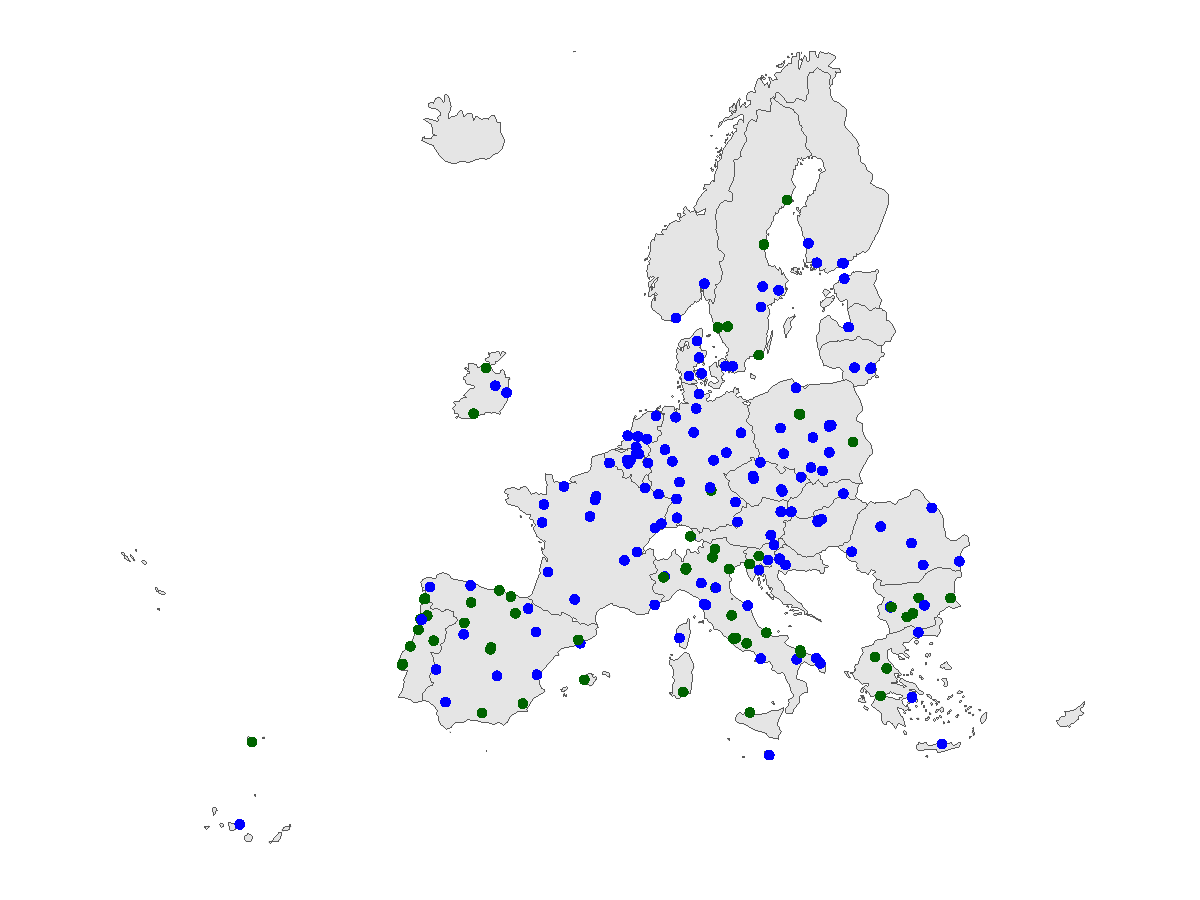
\includegraphics[width=0.6\textwidth, trim={160 23 80 0}, clip]{../Output/EDIH_and_Seal_of_Excellence_map.pdf}
    \end{figure}
\end{frame}

\begin{frame}{The DMA Survey - Design}
    \begin{itemize}
        \item In 2021, European Commission tasks the Joint Research Centre (JRC) with the design of a survey to evaluate the success of the EDIH initiative
        \item Focus on the measure of Digital Maturity across six dimensions:
        \begin{figure}
            \centering
            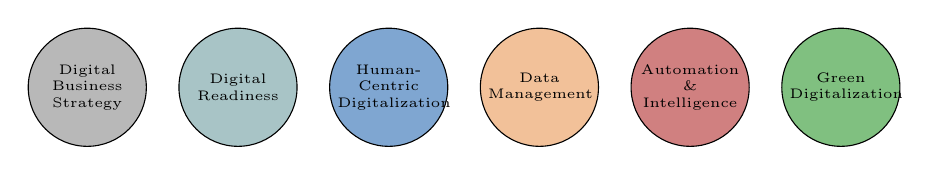
\begin{tikzpicture}[node distance=0.05cm] % Adjust spacing between nodes
                % Define the circles with fixed size and constrained text width
                \node[circle,draw,minimum size=1.5cm,inner sep=0pt,fill=color1,align=center] (c1) {\parbox{1.3cm}{\centering \tiny Digital \\ \tiny Business \\ \tiny Strategy}};
                \node[circle,draw,minimum size=1.5cm,inner sep=0pt,fill=color2,align=center, right=0.4cm of c1] (c2) {\parbox{1.3cm}{\centering \tiny Digital \\ \tiny Readiness}};
                \node[circle,draw,minimum size=1.5cm,inner sep=0pt,fill=color3,align=center, right=0.4cm of c2] (c3) {\parbox{1.3cm}{\centering \tiny Human-Centric \\ \tiny Digitalization}};
                \node[circle,draw,minimum size=1.5cm,inner sep=0pt,fill=color4,align=center, right=0.4cm of c3] (c4) {\parbox{1.3cm}{\centering \tiny Data \\ \tiny Management}};
                \node[circle,draw,minimum size=1.5cm,inner sep=0pt,fill=color5,align=center, right=0.4cm of c4] (c5) {\parbox{1.3cm}{\centering \tiny Automation \\ \tiny \& Intelligence}};
                \node[circle,draw,minimum size=1.5cm,inner sep=0pt,fill=color6,align=center, right=0.4cm of c5] (c6) {\parbox{1.3cm}{\centering \tiny Green \\ \tiny Digitalization}};
            \end{tikzpicture}
        \end{figure}
        \item Survey submitted by firms using the EDIH services at 3 points in time:
    \end{itemize}
    \begin{figure}
        \centering
        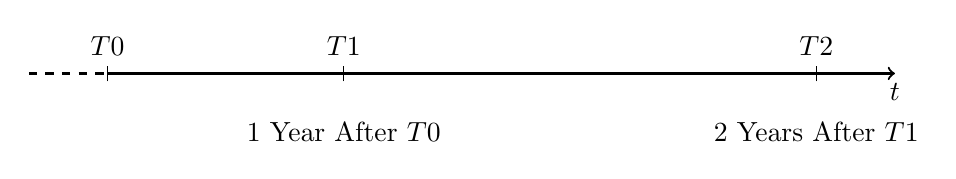
\begin{tikzpicture}
            % Draw the timeline arrow with dashed line at the beginning
            \draw[dashed, thick] (0,0) -- (1,0);
            \draw[->, thick] (1,0) -- (11,0) node[anchor=north] {$t$};
    
            % Draw the points t0, t1, t2 at mid height
            \foreach \x/\label in {1/$T0$, 4/$T1$, 10/$T2$} {
                \draw (\x,-0.1) -- (\x,0.1) node[anchor=south] {\label};
            }
    
            % Optional: Add labels below the timeline
            \node[anchor=north] at (1,-0.5) { };
            \node[anchor=north] at (4,-0.5) {1 Year After $T0$};
            \node[anchor=north] at (10,-0.5) {2 Years After $T1$};
        \end{tikzpicture}
        \caption{Timeline of DMA Submissions}
        \label{fig:timeline}
    \end{figure}
\end{frame}

\begin{frame}{The Research Question}
    \begin{itemize}
        \item EDIHs started operating in late 2023 $\to$ we only have data for $T0$ and (a very limited number of) $T1$ obs.
        %\item Thus, \textbf{no evaluation of the EDIH initiative is possible yet}.
        \item Research Question: \textbf{What leads firms to participate in the EDIH initiative?}
        \item Question is relevant w.r.t.:
            \begin{itemize}
                \item \textbf{Revisions of the initiative}
                \item \textbf{Future impact evaluation} (size of potential bias in the estimate).
            \end{itemize} 
        \item Hypothesis: drivers of participation are both \textbf{financial and non-financial factors} (including \textbf{geospatial characteristics}).
    \end{itemize}
\end{frame}

\begin{frame}{Methodology - Construction of the sample}
    \begin{enumerate}
        \item \textbf{Matching} of 3204 treated firms with ORBIS (using Jaro-Winkler distance) $\to$ 90\% matched $\to$ \textbf{firm-level data for treated group}.  
        \item \textbf{Construction} of a \textbf{synthetic control group} of untreated firms randomly sampled from the ORBIS database $\to$ \textbf{firm-level data for control group}.
        \item \textbf{Geocoding} of both treated and control groups: \\ input address $\to$ output coordinates.
        \item \textbf{Compute} 
            \begin{itemize}
                 \item \textbf{Haversine distance} of each firm to the closest EDIH
                 \item \textbf{\hyperlink{firm_density_slide}{Firm Density}} within 5 km radius of each firm (w/o EDIHs)
            \end{itemize}
        \item Final sample: \textbf{1249 treated} firms and \textbf{3643 controls}.
    \end{enumerate}
\end{frame}

\begin{frame}{Macrosectors compared: Treated vs Control}
    \begin{figure}
        \centering
            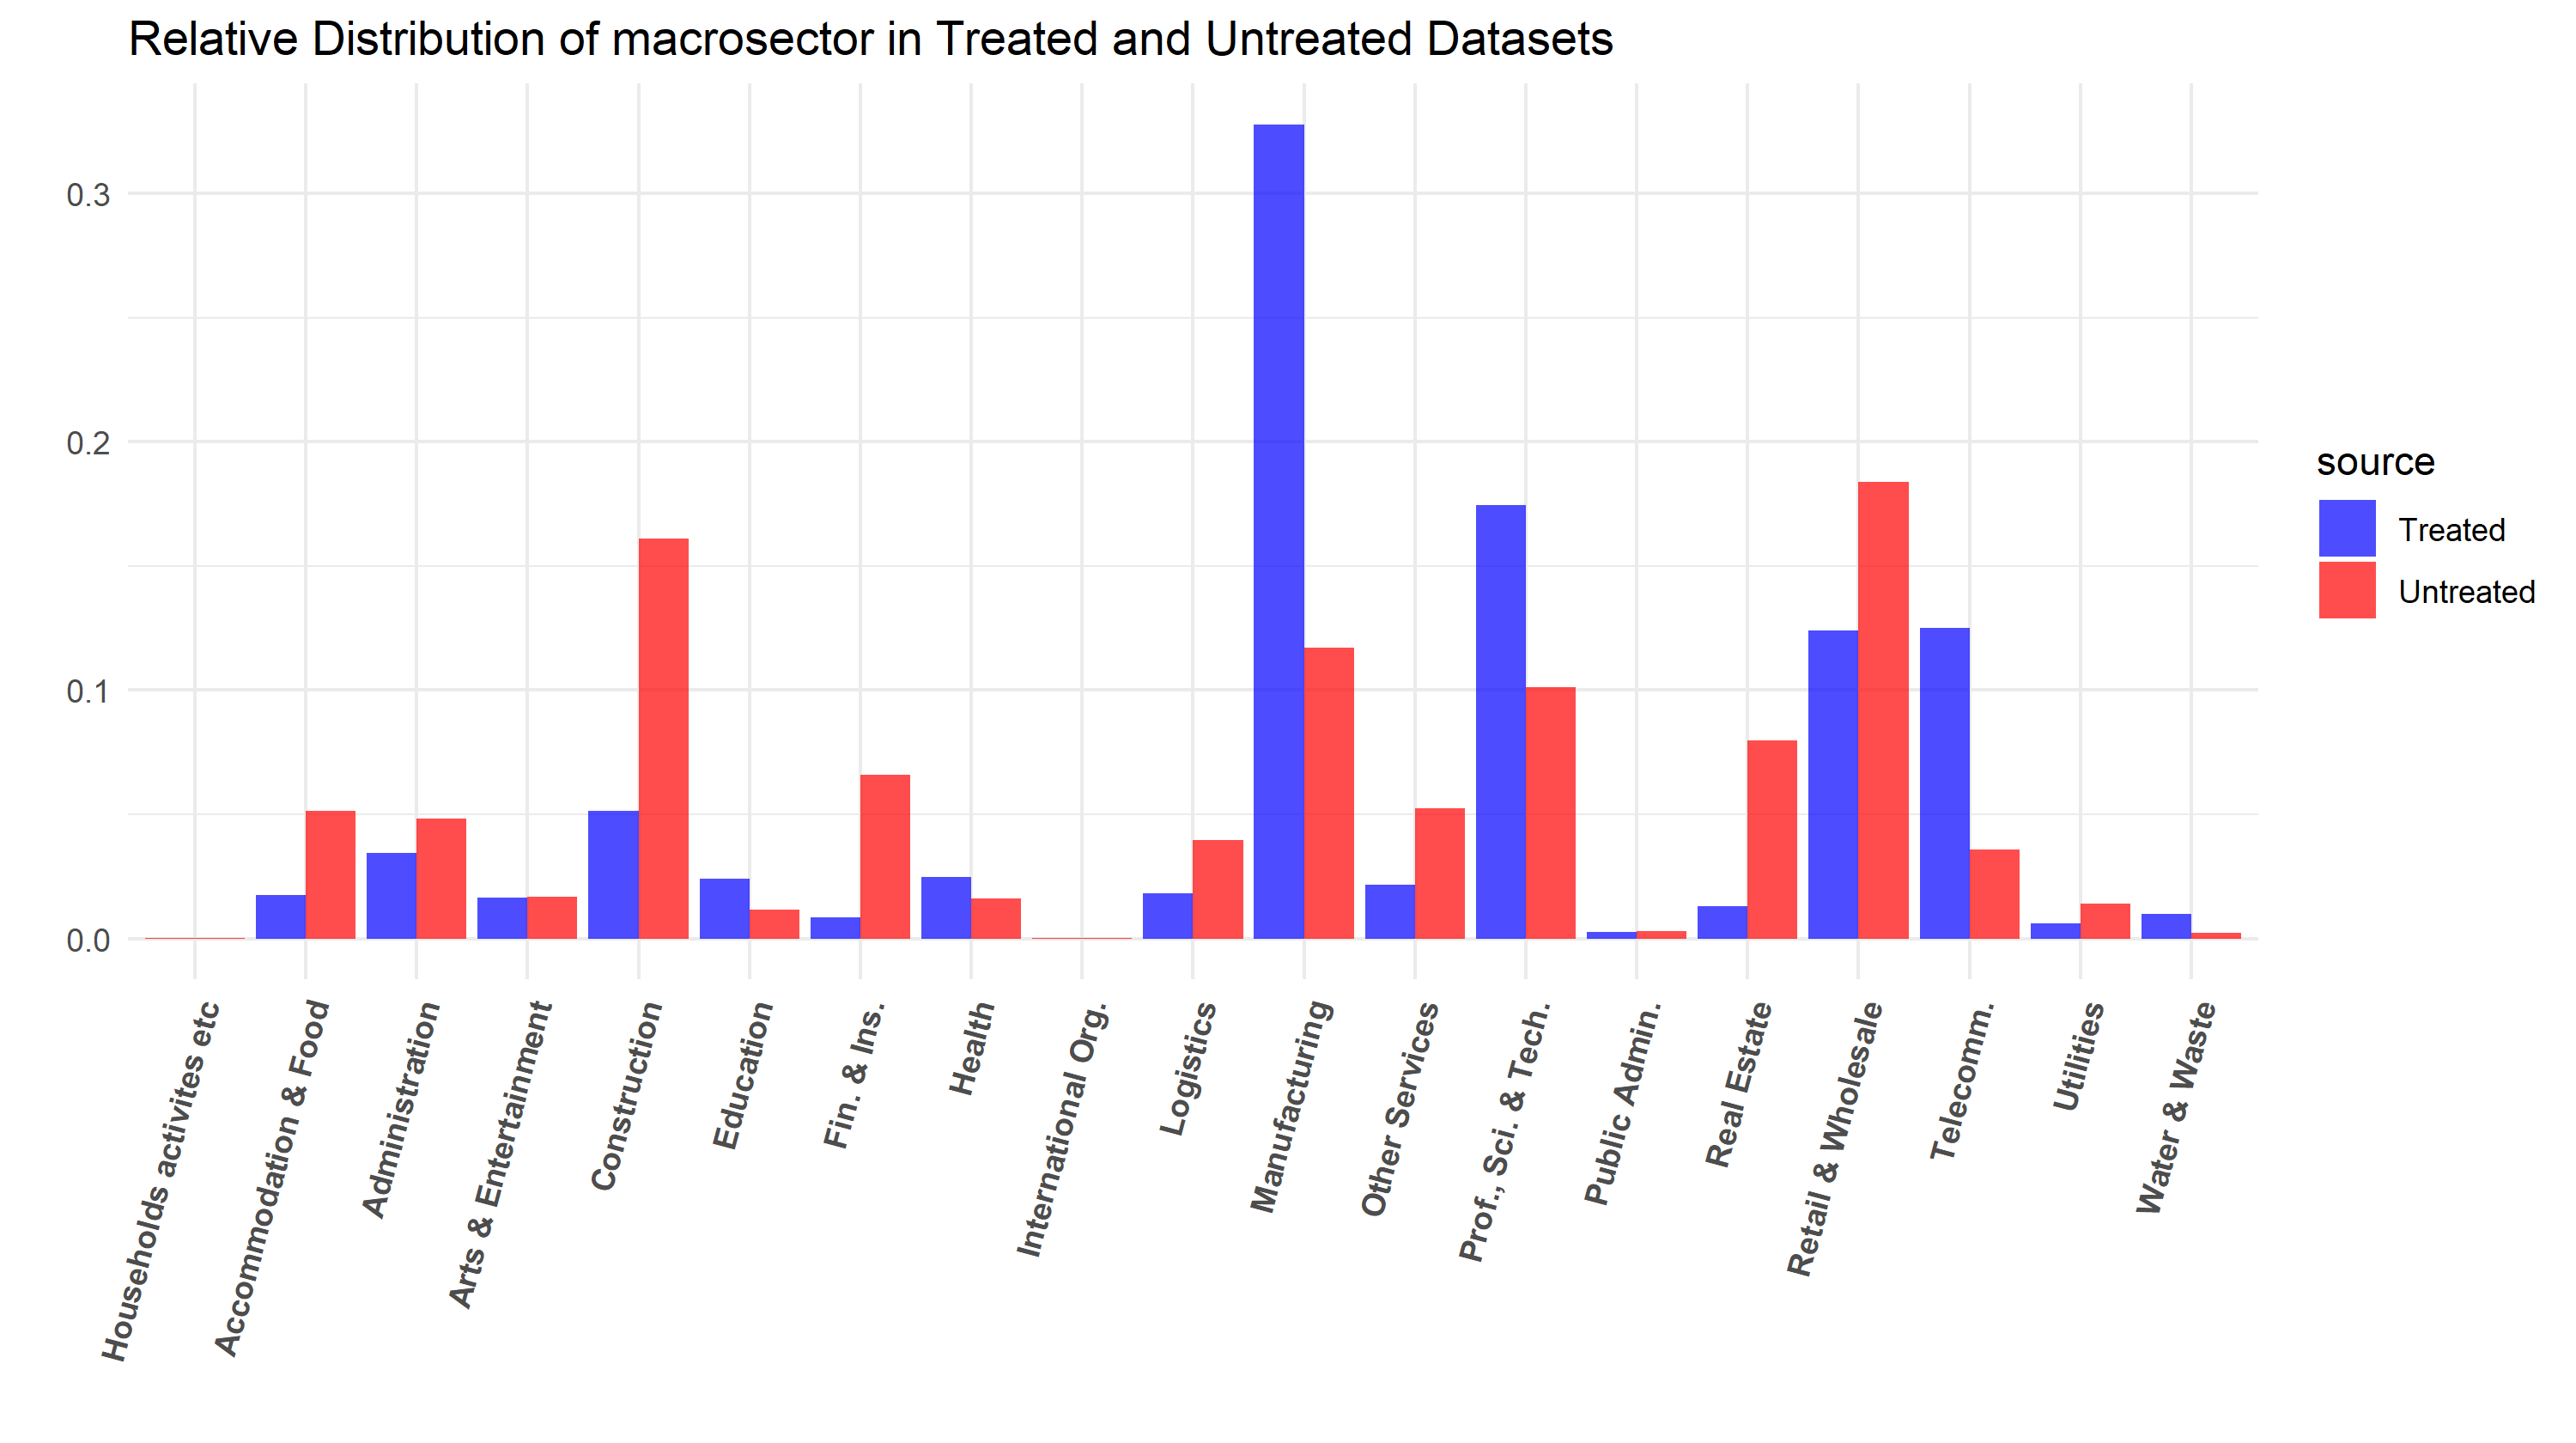
\includegraphics[width=0.9\textwidth, trim={0 23 80 0}, clip]{../Output/macrosectorsplot_compared.png}
            % Add legend below the figure with smaller characters
            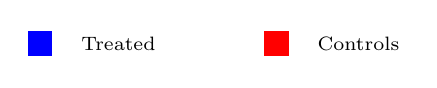
\begin{tikzpicture}
                % Blue square for Treated
                \node[rectangle, draw=blue, fill=blue, minimum size=0.3cm] (blue) at (0, 0) {};
                \node[anchor=west, font=\scriptsize] at (0.4, 0) {Treated};
                % Red square for Controls
                \node[rectangle, draw=red, fill=red, minimum size=0.3cm] (red) at (3, 0) {};
                \node[anchor=west, font=\scriptsize] at (3.4, 0) {Controls};
            \end{tikzpicture}
    \end{figure}
\end{frame}

\begin{frame}{Location compared: Treated...}
    \begin{figure}
        \centering
        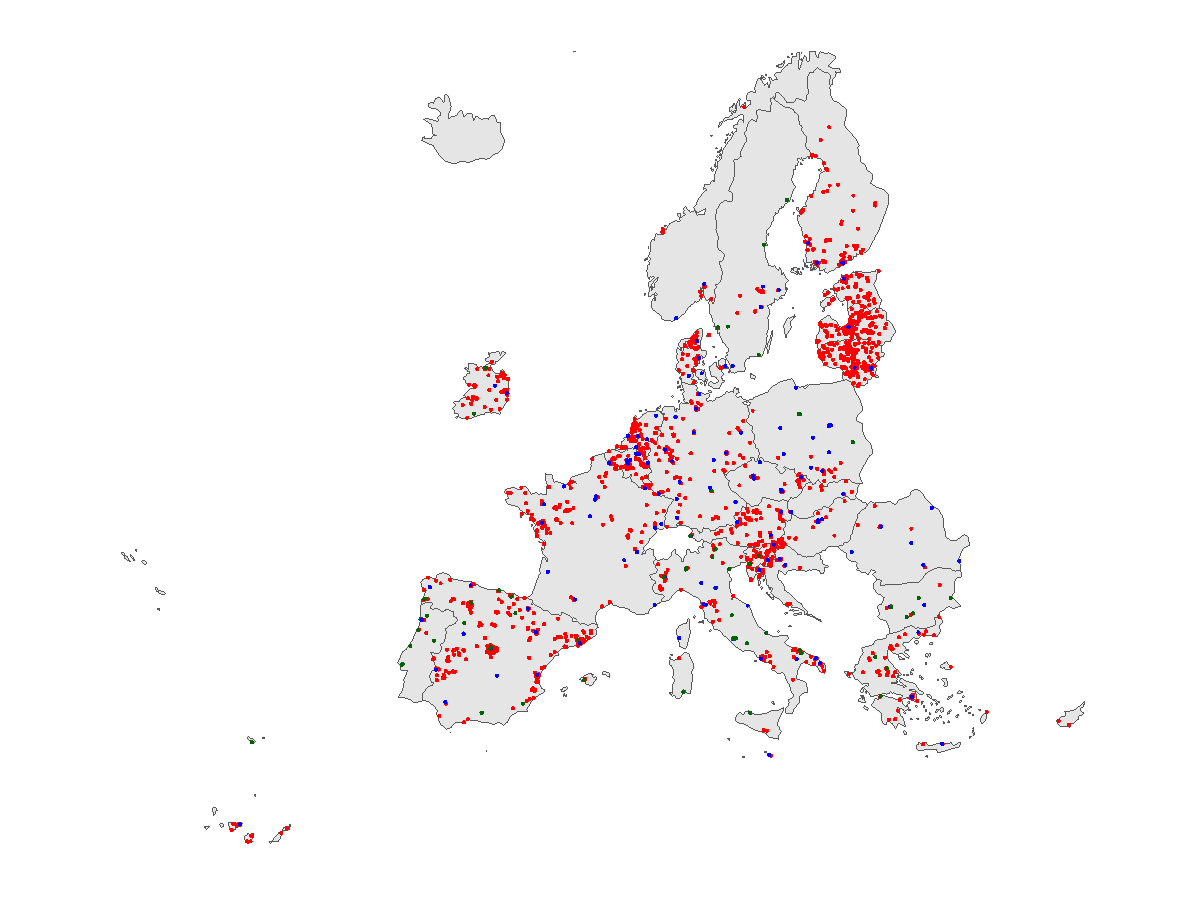
\includegraphics[width=0.6\textwidth, trim={175 50 50 20}, clip]{../Output/EU_map_onlytreated.pdf}
    \end{figure}
\end{frame}

\begin{frame}{...vs Control}
    \begin{figure}
        \centering
        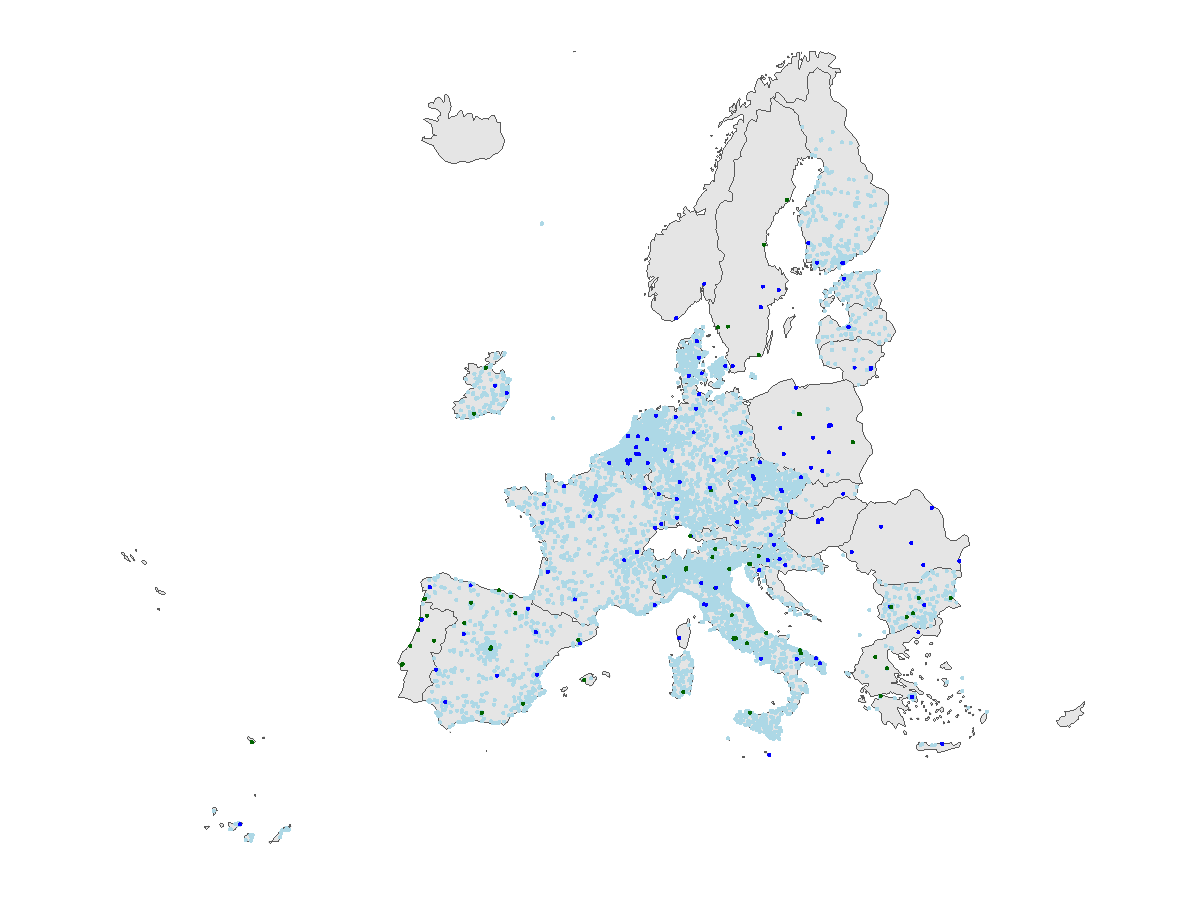
\includegraphics[width=0.6\textwidth, trim={175 50 50 20}, clip]{../Output/EU_map_onlysample.pdf}
    \end{figure}
\end{frame}


\begin{frame}{Methodology - Model Specification}
    \begin{itemize}
        \item Estimate a Probit model with the following specification: 
        \begin{equation*}
        \begin{split}
            D_{i}(\text{Treated}_{i} = 1) = \beta_{0} &+ \beta_{1} \text{Distance}_{i} + \beta_{2} \text{Firm Density}_{i} \\
            &+ \beta_{3} \text{Sector}_{i} + \beta_{4} \text{Tech Level}_{i} \\
            &+ \beta_{5} \text{Turnover}_{i} + \beta_{6} \text{Employees}_{i} \\
            &+ \beta_{7} \text{Liquidity Ratio}_{i} + \beta_{8} \text{Solvency Ratio}_{i} \\
            &+ \beta_{9} \text{Country Group}_{i} + \varepsilon_{i}
        \end{split}
    \end{equation*}
    \item Variations:
        \begin{itemize}
            \item Model 1: Without distance and firm density.
            \item Model 2: With distance and without firm density.
            \item Model 3: With both firm density and distance (Model 3 is run on the whole sample and then on macrosectoral subsamples).
        \end{itemize}
    \end{itemize}
\end{frame}

\begin{frame}{Regression Results - Coefficients}
    \begin{tikzpicture}[remember picture, overlay]
        % Example of overlaying rectangles with thick borders and no fill
        % Adjust the coordinates (x1, y1) and (x2, y2) to position the rectangles
        \draw[blue, thick] (7.9, -5) rectangle (9.7, -7); % Example rectangle 1
        \draw[blue, thick] (7.9, -1.03) rectangle (9.7, -2.03); % Example rectangle 2
    \end{tikzpicture}
    
% Table created by stargazer v.5.2.3 by Marek Hlavac, Social Policy Institute. E-mail: marek.hlavac at gmail.com
% Date and time: dom, gen 19, 2025 - 23:36:24
\begin{table}[!htbp] \centering
\tiny
\renewcommand{\arraystretch}{1} 
  \label{} 
\begin{tabular}{@{\extracolsep{5pt}}lccc} 
\\[-1.8ex]\hline 
\hline 
\\[-1.8ex] & \multicolumn{3}{c}{treated} \\ 
 & w/o Dist & w/ Dist & w/ Dist and Dens \\ 
\hline \\[-1.8ex] 
 Dist. from EDIH &  & $-$0.002$^{***}$ & $-$0.002$^{***}$ \\ 
  &  & (0.0004) & (0.0004) \\ 
  
 Firm Density &  &  & 0.001$^{***}$ \\ 
  &  &  & (0.0005) \\ 
   
 Manufacturing & 0.328$^{***}$ & 0.337$^{***}$ & 0.361$^{***}$ \\ 
  & (0.103) & (0.103) & (0.103) \\ 
   
 Services & 0.269$^{***}$ & 0.245$^{***}$ & 0.222$^{***}$ \\ 
  & (0.074) & (0.074) & (0.074) \\ 
   
 High Tech & 1.260$^{***}$ & 1.233$^{***}$ & 1.216$^{***}$ \\ 
  & (0.181) & (0.182) & (0.183) \\ 

 Medium-High Tech & 1.592$^{***}$ & 1.554$^{***}$ & 1.539$^{***}$ \\ 
  & (0.088) & (0.089) & (0.089) \\ 
   
 Medium Tech & 0.783$^{***}$ & 0.766$^{***}$ & 0.749$^{***}$ \\ 
  & (0.143) & (0.144) & (0.144) \\ 
 
 Medium-Low Tech & 0.774$^{***}$ & 0.745$^{***}$ & 0.723$^{***}$ \\ 
  & (0.070) & (0.071) & (0.072) \\ 
 
 Turnover & $-$0.0004 & $-$0.0004 & $-$0.0004 \\ 
  & (0.0005) & (0.0005) & (0.0005) \\ 
  
 Employees & 0.768$^{***}$ & 0.749$^{***}$ & 0.741$^{***}$ \\ 
  & (0.165) & (0.165) & (0.164) \\ 
 
 Liquidity Ratio & $-$0.092$^{***}$ & $-$0.094$^{***}$ & $-$0.095$^{***}$ \\ 
  & (0.009) & (0.009) & (0.009) \\ 
  
 Solvency Ratio & 0.010$^{***}$ & 0.010$^{***}$ & 0.010$^{***}$ \\ 
  & (0.001) & (0.001) & (0.001) \\ 

\hline \\[-1.8ex] 
Observations & 4,864 & 4,864 & 4,864 \\
\hline 
\hline \\[-1.8ex] 
\textit{Note:}  & \multicolumn{3}{r}{$^{*}$p$<$0.1; $^{**}$p$<$0.05; $^{***}$p$<$0.01} \\ 
\end{tabular} 
\end{table} 

\end{frame}

\begin{frame}{Regression Results - Average Marginal Effects}
    \begin{tikzpicture}[remember picture, overlay]
        % Example of overlaying rectangles with thick borders and no fill
        % Adjust the coordinates (x1, y1) and (x2, y2) to position the rectangles
        \draw[blue, thick] (3.7, -4.25) rectangle (4.9, -5.83); % Example rectangle 1
        \draw[blue, thick] (3.7, -1.13) rectangle (4.9, -2.42); % Example rectangle 2
    \end{tikzpicture}
    % Table created by stargazer v.5.2.3 by Marek Hlavac, Social Policy Institute. E-mail: marek.hlavac at gmail.com
% Date and time: dom, gen 19, 2025 - 23:36:32
\begin{table}[!htbp] \centering
  \footnotesize
    \renewcommand{\arraystretch}{1} 
      \label{} 
\begin{tabular}{@{\extracolsep{5pt}} cccccc} 
\\[-1.8ex]\hline 
\hline \\[-1.8ex] 
factor & AME & SE & p & lower & upper \\ 
\hline \\[-1.8ex] 
Dist. from EDIH & $$-$0.0003$ & $0.0001$ & $0.0003$ & $$-$0.0005$ & $$-$0.0001$ \\ 
Employees & $0.143$ & $0.032$ & $0.00001$ & $0.082$ & $0.205$ \\ 
Firm Density & $0.0003$ & $0.0001$ & $0.002$ & $0.0001$ & $0.0005$ \\ 
Liquidity Ratio & $$-$0.018$ & $0.002$ & $0$ & $$-$0.022$ & $$-$0.015$ \\ 
Turnover & $$-$0.0001$ & $0.0001$ & $0.450$ & $$-$0.0003$ & $0.0001$ \\ 
Manufacturing & $0.071$ & $0.021$ & $0.001$ & $0.030$ & $0.111$ \\ 
Services & $0.042$ & $0.014$ & $0.002$ & $0.015$ & $0.069$ \\ 
Solvency Ratio & $0.002$ & $0.0002$ & $0$ & $0.002$ & $0.002$ \\ 
High Tech & $0.290$ & $0.050$ & $0$ & $0.191$ & $0.389$ \\ 
Medium Tech & $0.164$ & $0.036$ & $0.00001$ & $0.093$ & $0.235$ \\ 
Medium-High Tech & $0.380$ & $0.023$ & $0$ & $0.334$ & $0.426$ \\ 
Medium-Low Tech & $0.157$ & $0.017$ & $0$ & $0.124$ & $0.191$ \\ 
\hline \\[-1.8ex] 
\end{tabular} 
\end{table}

\end{frame}

\begin{frame}{Robustness Check - Country Effects on coefficients}
    \begin{figure}
        \centering
        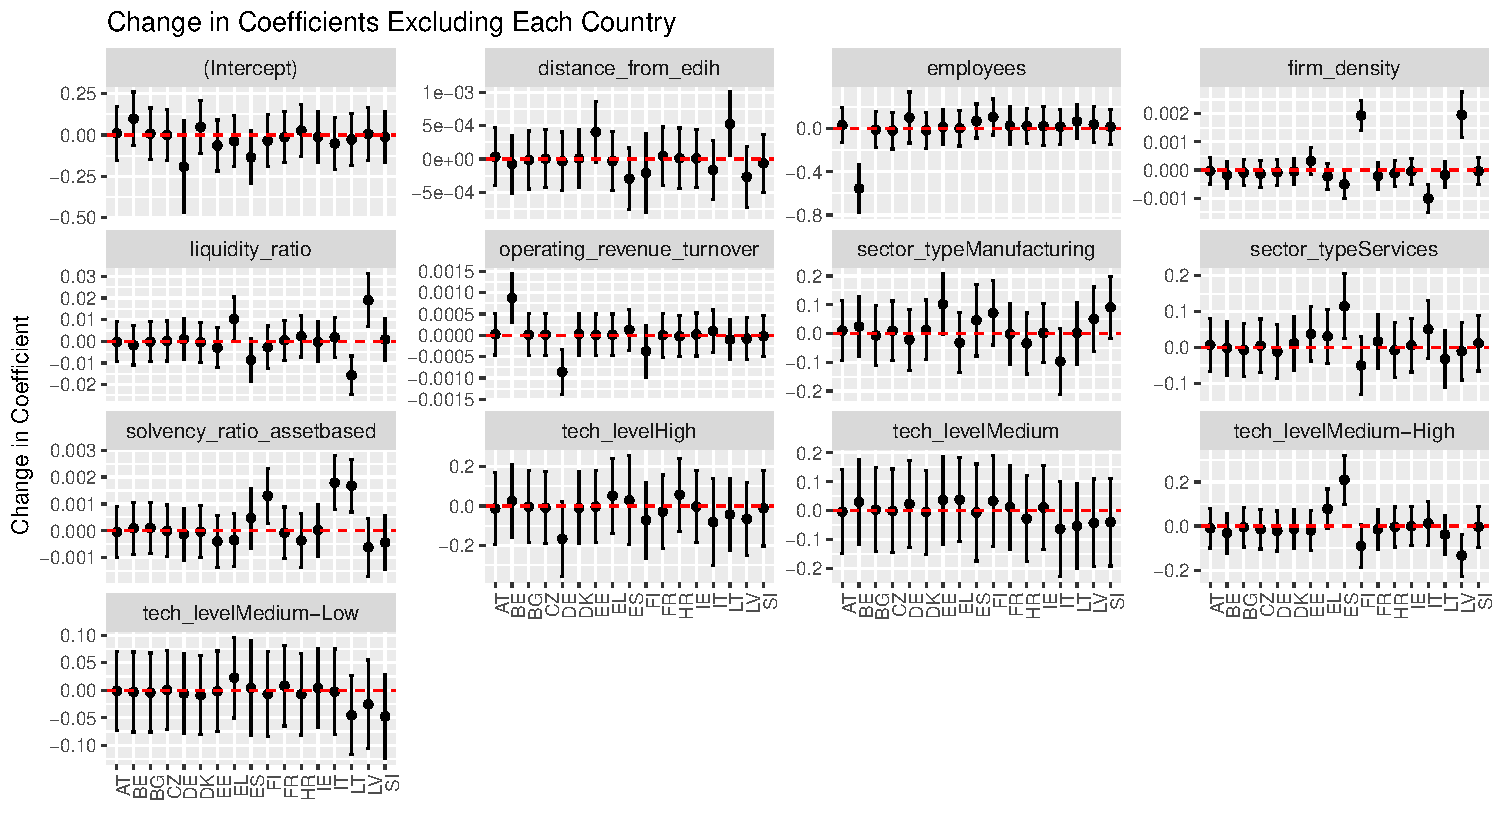
\includegraphics[width=1\textwidth]{../Output/changes-in-coeff-nocountryeffects-LEGACY.pdf}
        % Overlay the rectangle directly on the figure
    \begin{tikzpicture}[remember picture, overlay]
        % Adjust the coordinates to match the figure's dimensions
        \draw[blue, thick] (-2.8, 6.9) rectangle (6.1, 5.4); % Example rectangle, adjust as needed
    \end{tikzpicture}
    \end{figure}
\end{frame}

\begin{frame}{Conclusions, Policy Implications \& Future Research}

    \begin{itemize}
        \item Geospatial characteristics are drivers of participation in the EDIH initiative $\to$ \textbf{geographical distribution of EDIHs is key!}
        \item \textbf{Positive effect} of \textbf{size} and \textbf{solvency ratio} \& \textbf{negative} effect of \textbf{liquidity ratio} $\to$ \textbf{larger}, financially \textbf{stable} (but \textbf{liquidity-constrained!}) firms are \textbf{more likely to participate} $\to$ \textbf{correct targeting?}
        \item Country effects are significant $\to$ \textbf{EDIH's internal know-how is relevant!} $\to$ effect should taper down over time.
        \item Future work: \textbf{Impact evaluation} of the EDIH initiative on firm-level outcomes; \textbf{EDIH-level analysis} on effectiveness of the network approach.
    \end{itemize}
\end{frame}


% \begin{frame}
%     \begin{figure}
%         \centering
%         \begin{subfigure}[b]{0.45\textwidth}
%             \centering
%             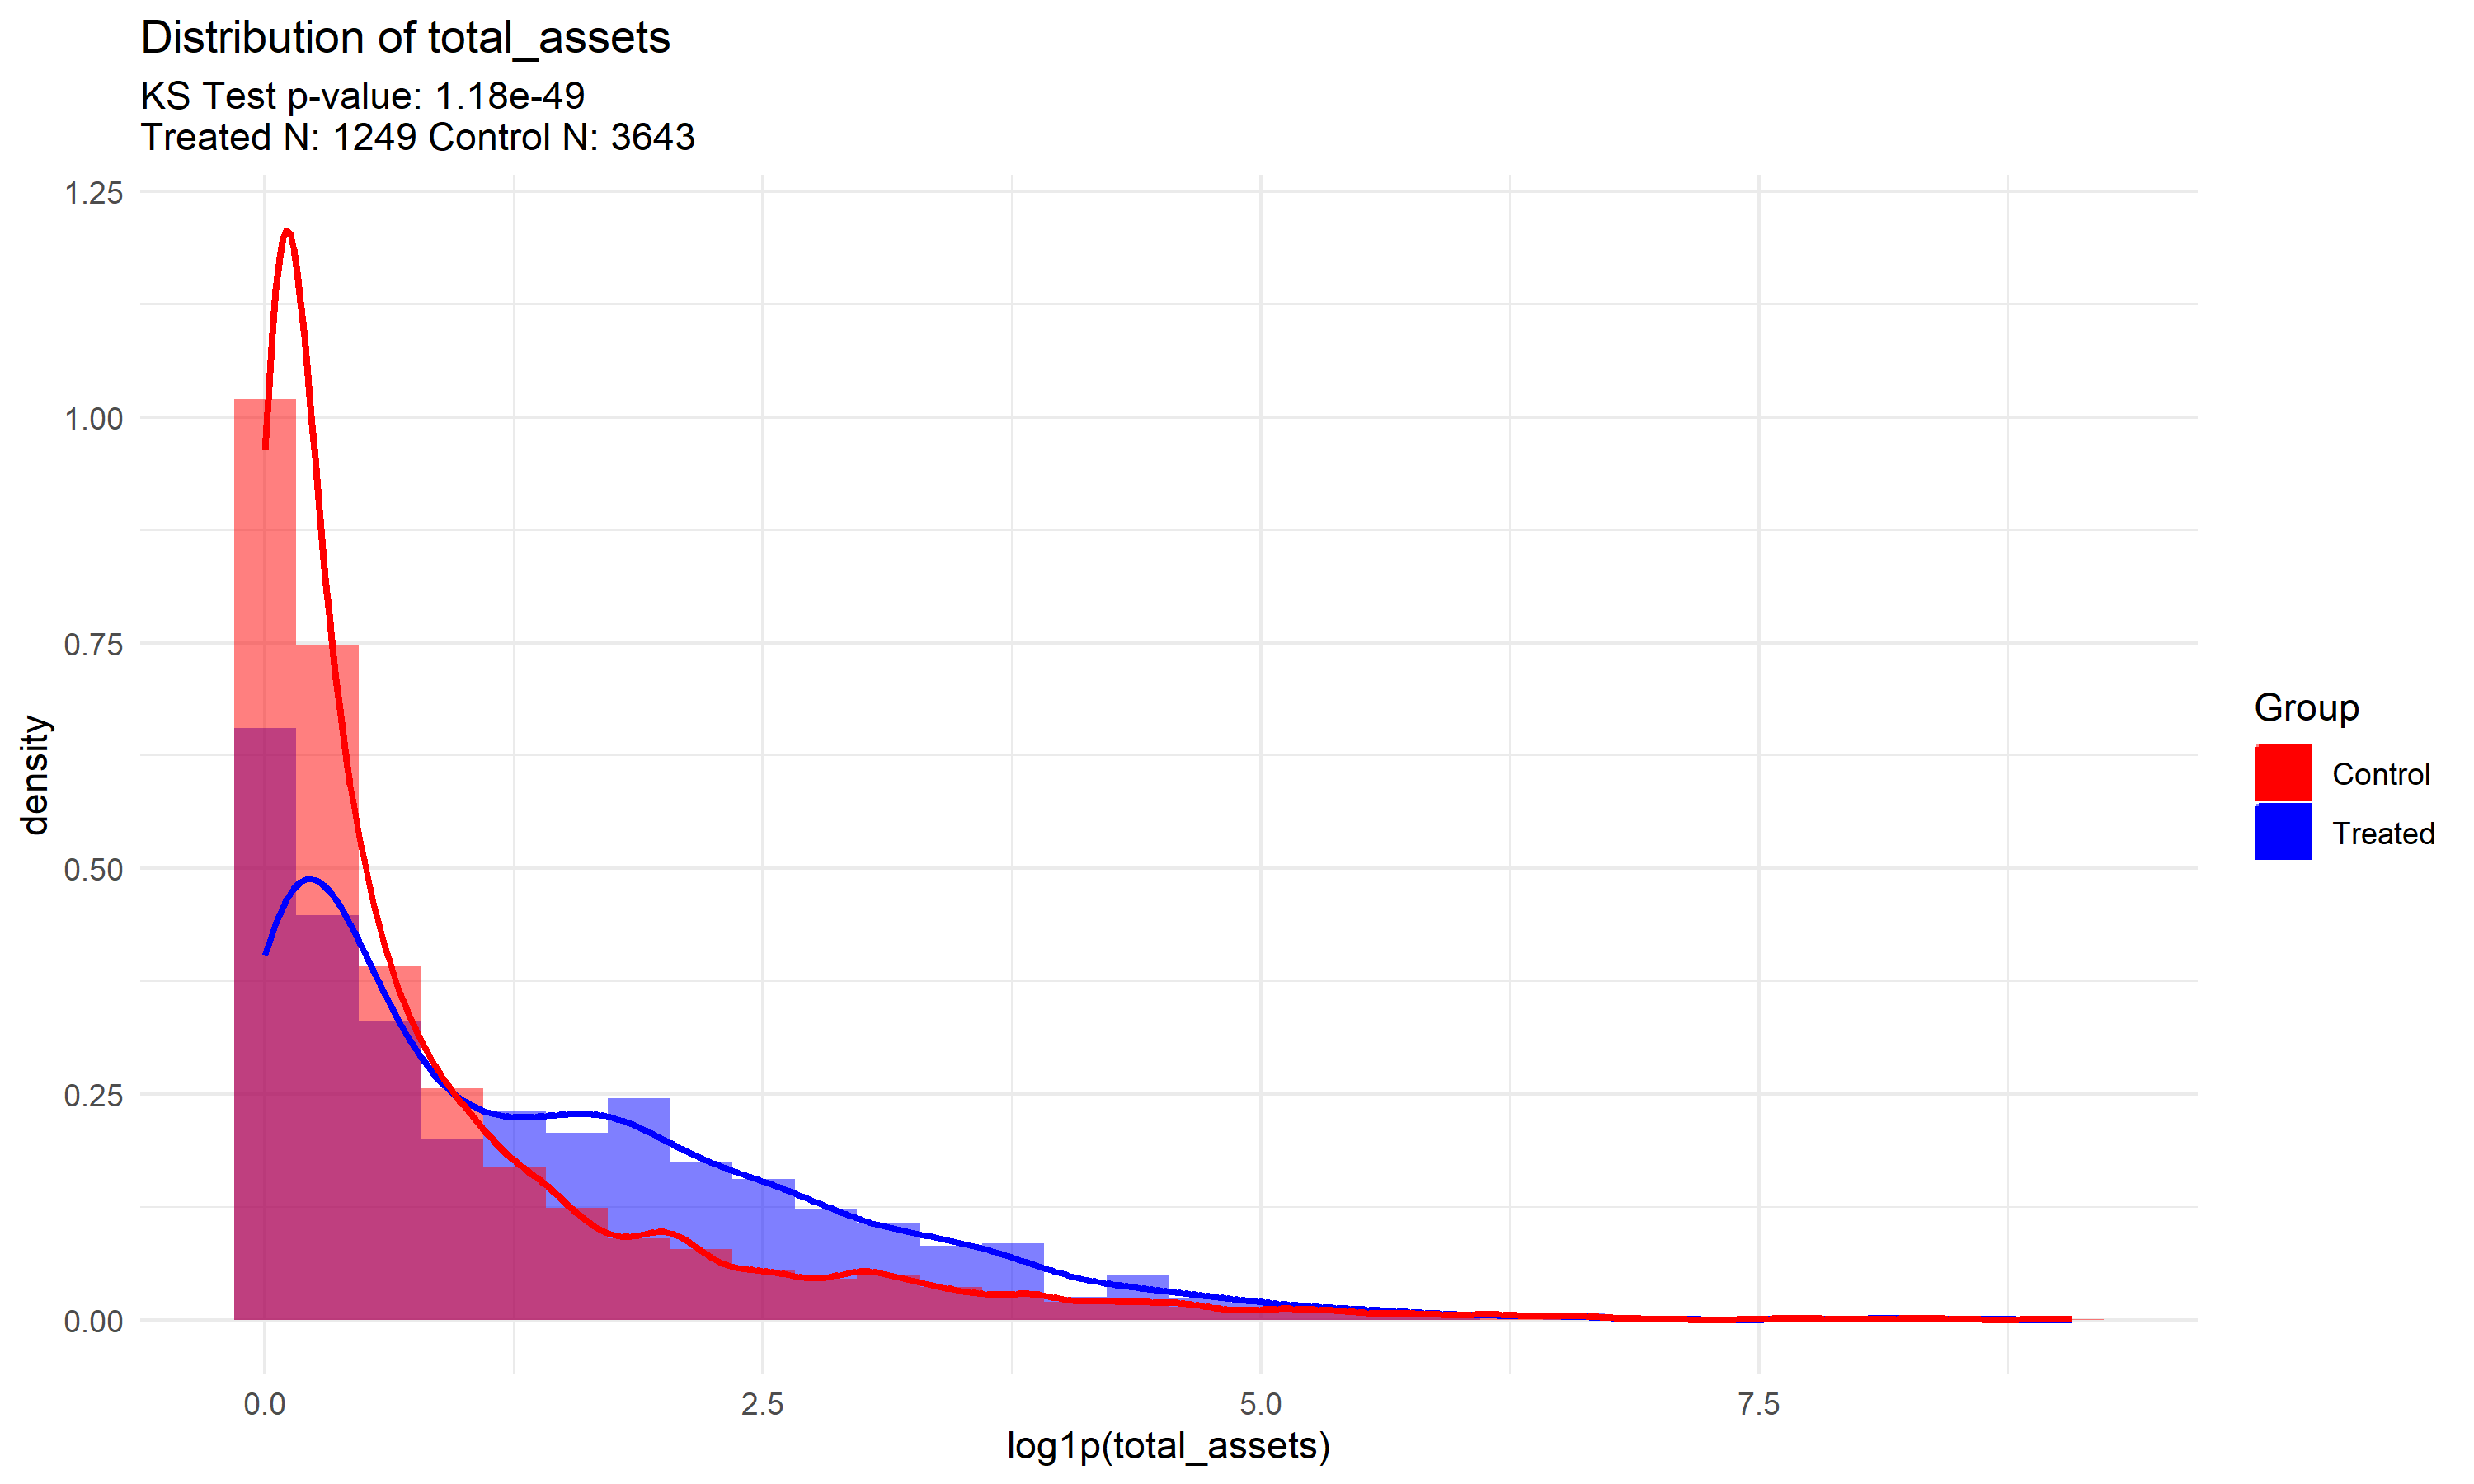
\includegraphics[width=\linewidth]{../Output/distrib_compare_total_assets_allcountries.png}
%             \caption{Total Assets}
%             \label{fig:total_assets}
%         \end{subfigure}
%         \hfill
%         \begin{subfigure}[b]{0.45\textwidth}
%             \centering
%             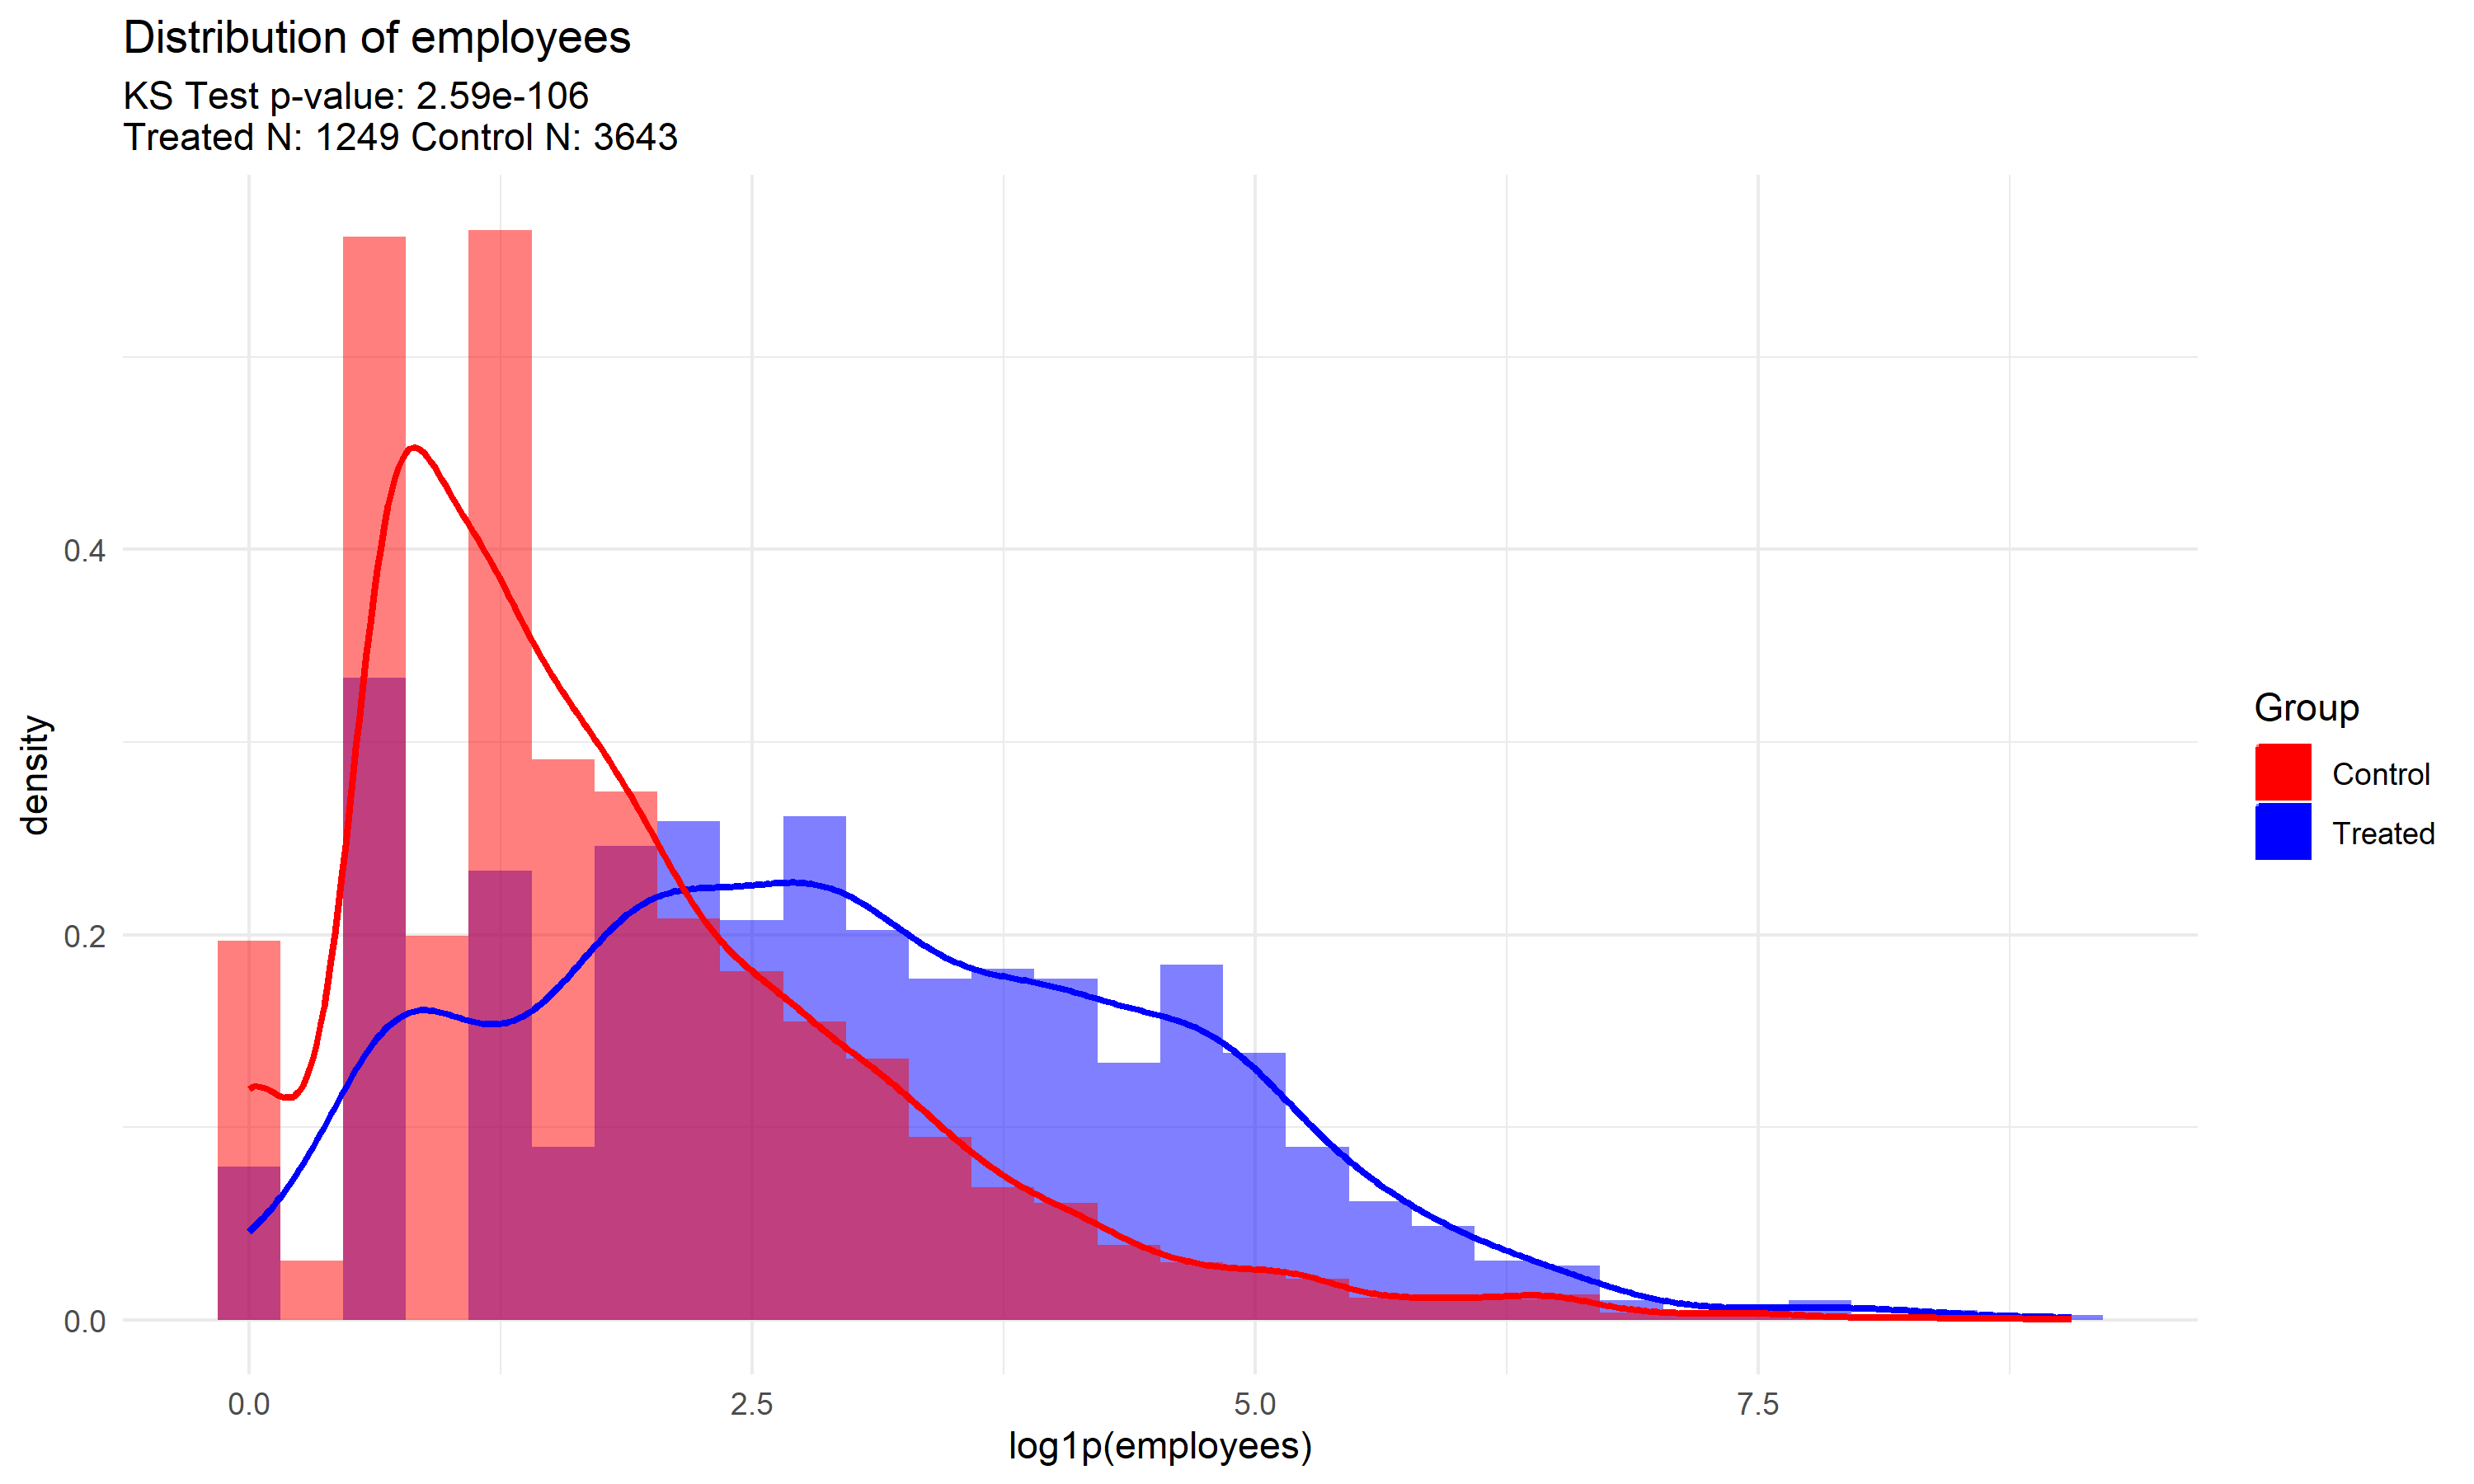
\includegraphics[width=\linewidth]{../Output/distrib_compare_employees_allcountries.png}
%             \caption{Employees}
%             \label{fig:employees}
%         \end{subfigure}
%         \caption{Distribution Comparisons Across All Countries}
%         \label{fig:distribution_comparisons_lotsofvasrs}
%     \end{figure}
% \end{frame}

\begin{frame}{The End}
    \centering
    \large\textbf{Thanks for Your Attention!}
    % \vspace{1cm}
    
    % \normalsize
    % Questions or Comments? \\
    % Feel free to reach out: \href{mailto:federico.vicentini@example.com}{federico.vicentini@example.com}
\end{frame}


    \begin{frame}{DMA - Question 1}
        \centering\textit{In which of the following business areas has your enterprise already invested in digitalisation and in
        which ones does it plan to in the future?}
        \begin{figure}
            \centering
            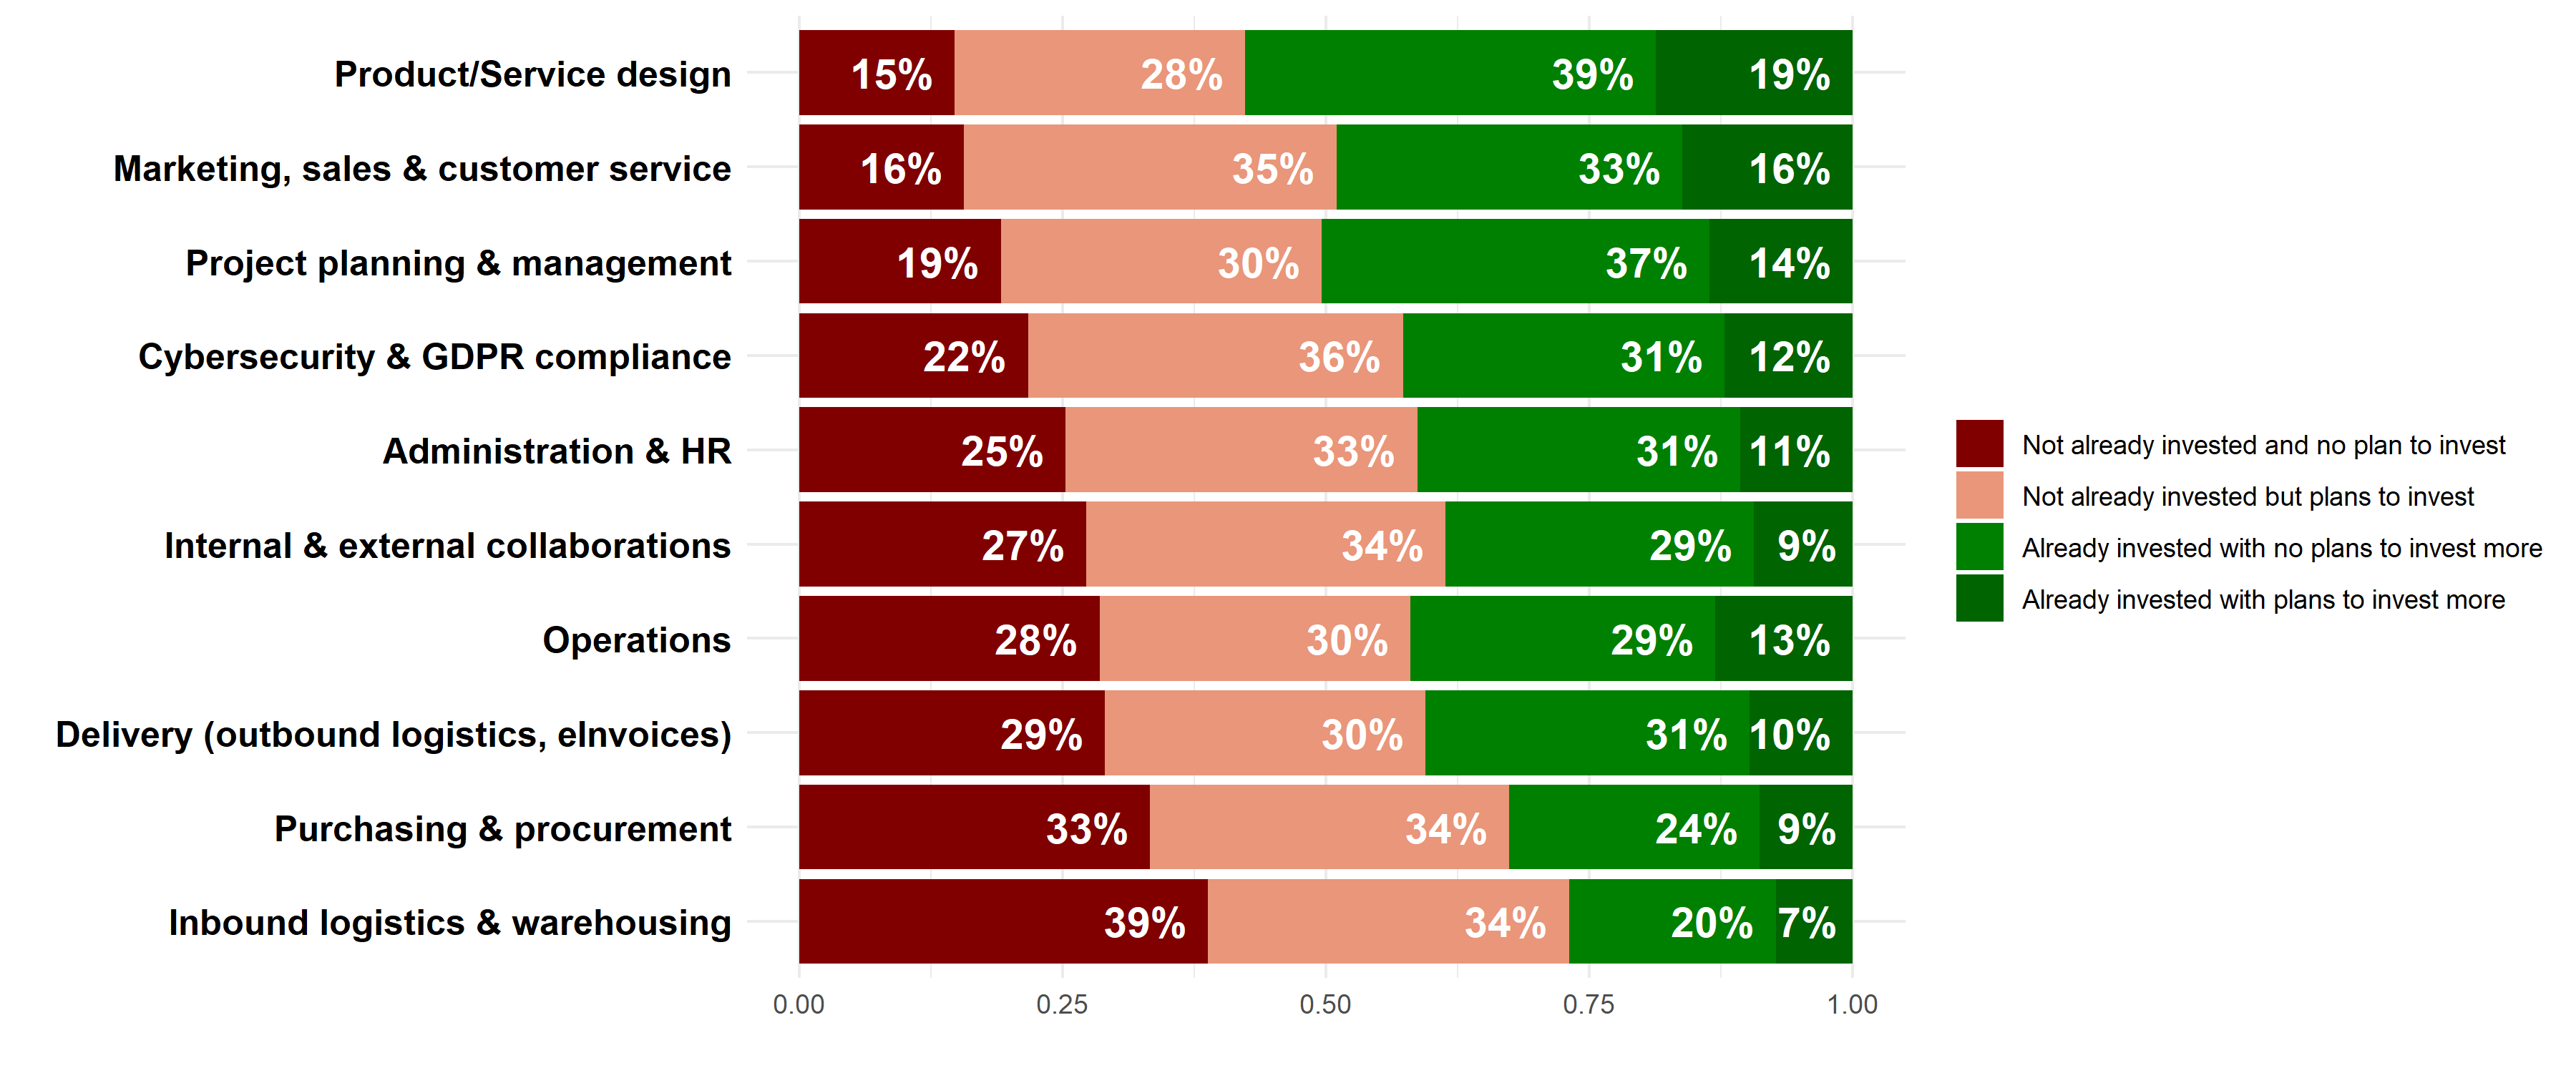
\includegraphics[width=\textwidth]{../Output/q1collapsed.png}

        \end{figure}
    \end{frame}



    \begin{frame}{DMA - Question 2}
        \centering\textit{In which of the following ways is your enterprise prepared for (more) digitalisation?}
        \begin{figure}
            \centering
            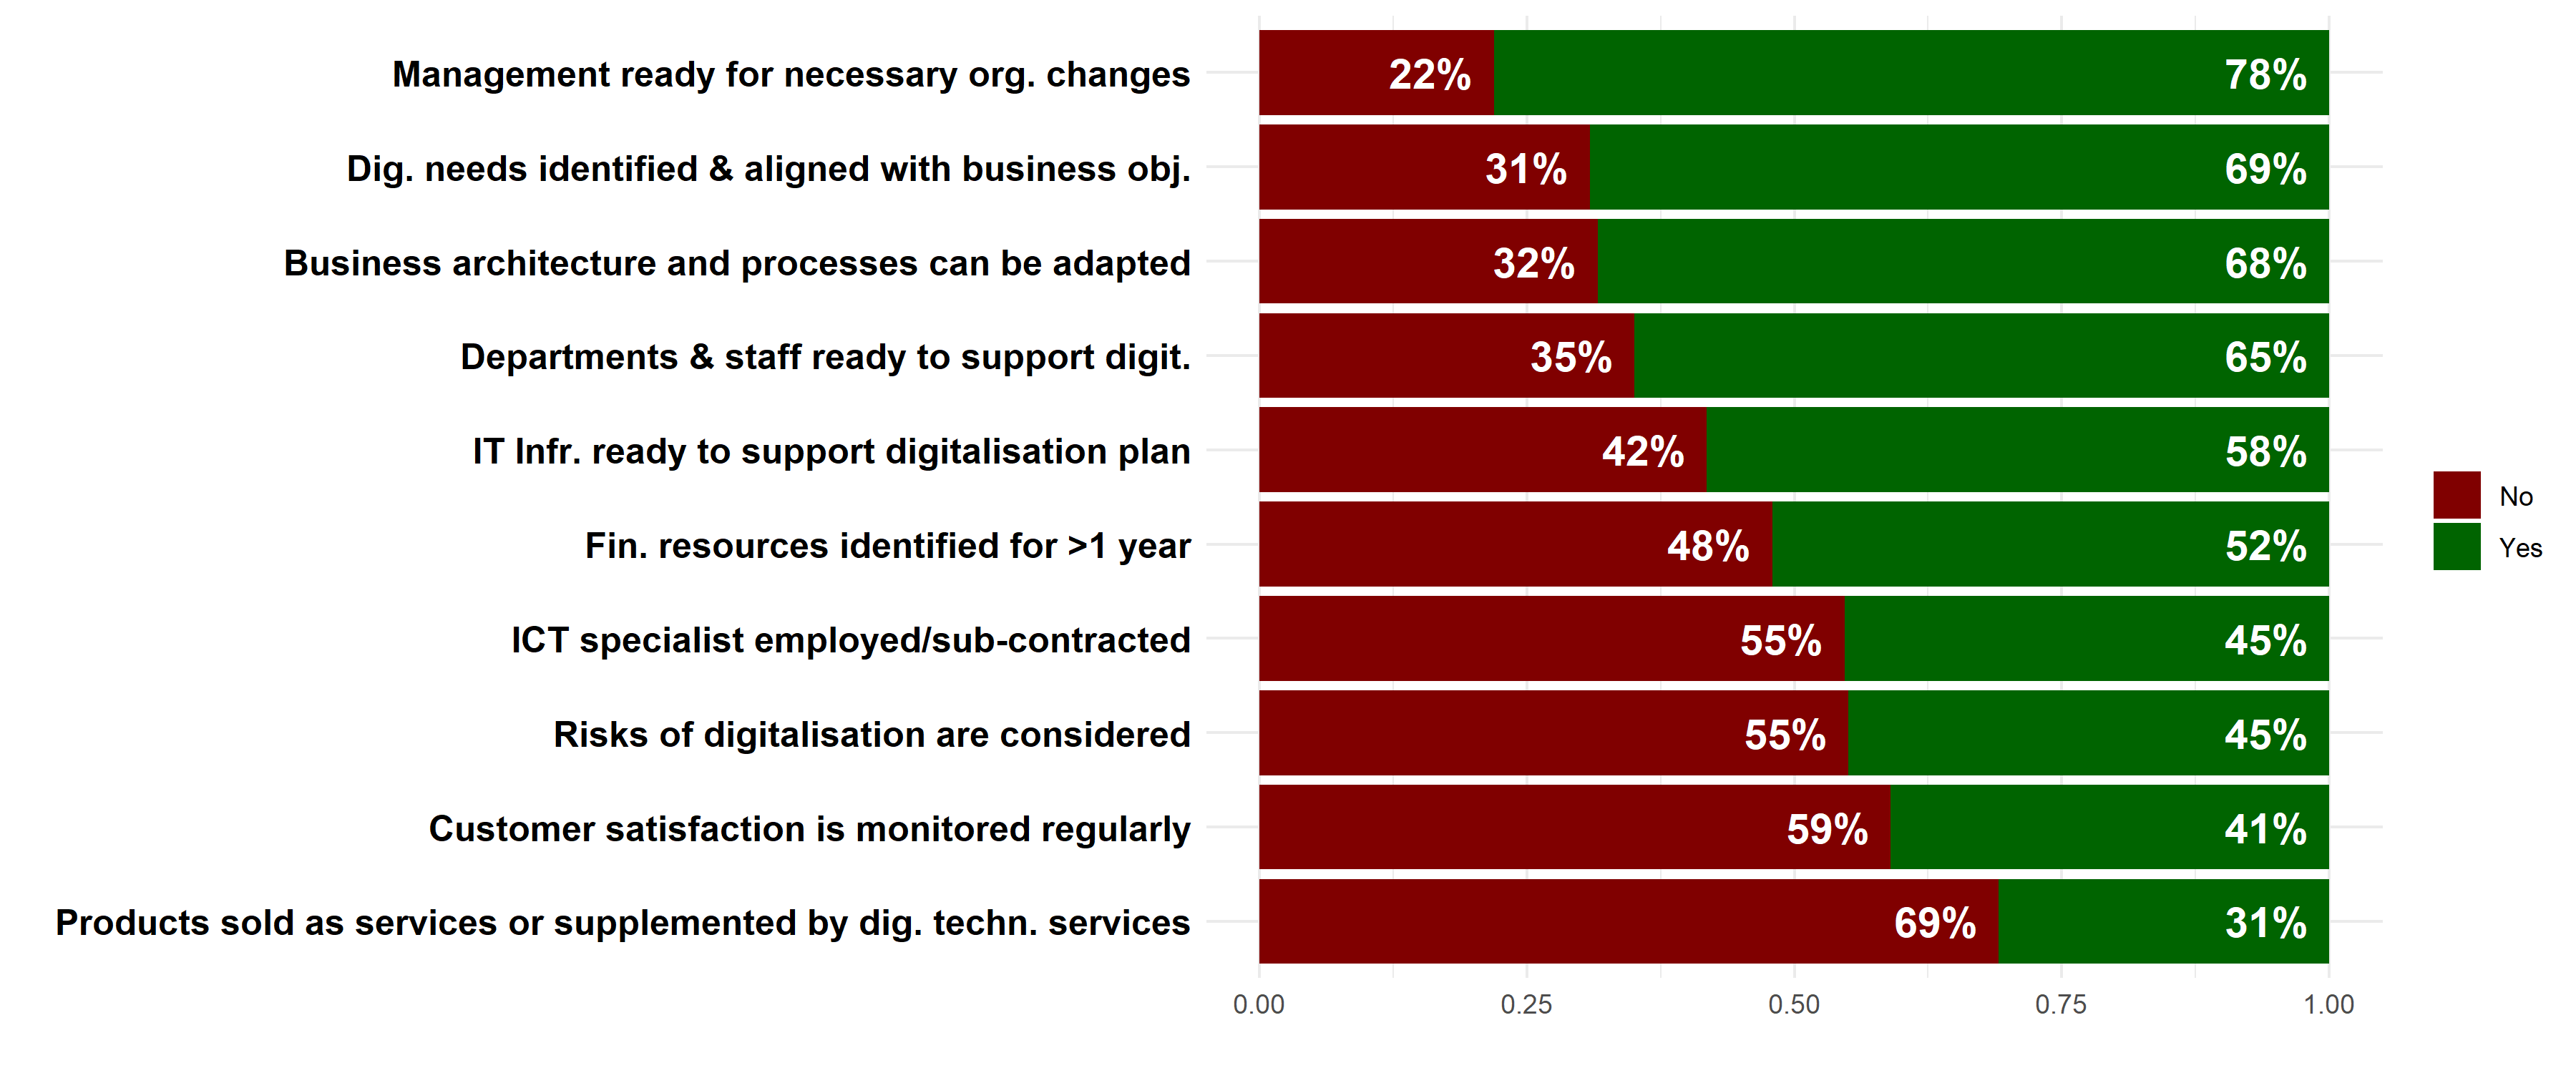
\includegraphics[width=\textwidth]{../Output/q2.png}

        \end{figure}
    \end{frame}

    \begin{frame}{DMA - Question 3}
        \centering\textit{Which of the following digital technologies and solutions are already used by your enterprise?}
        \begin{figure}
            \centering
            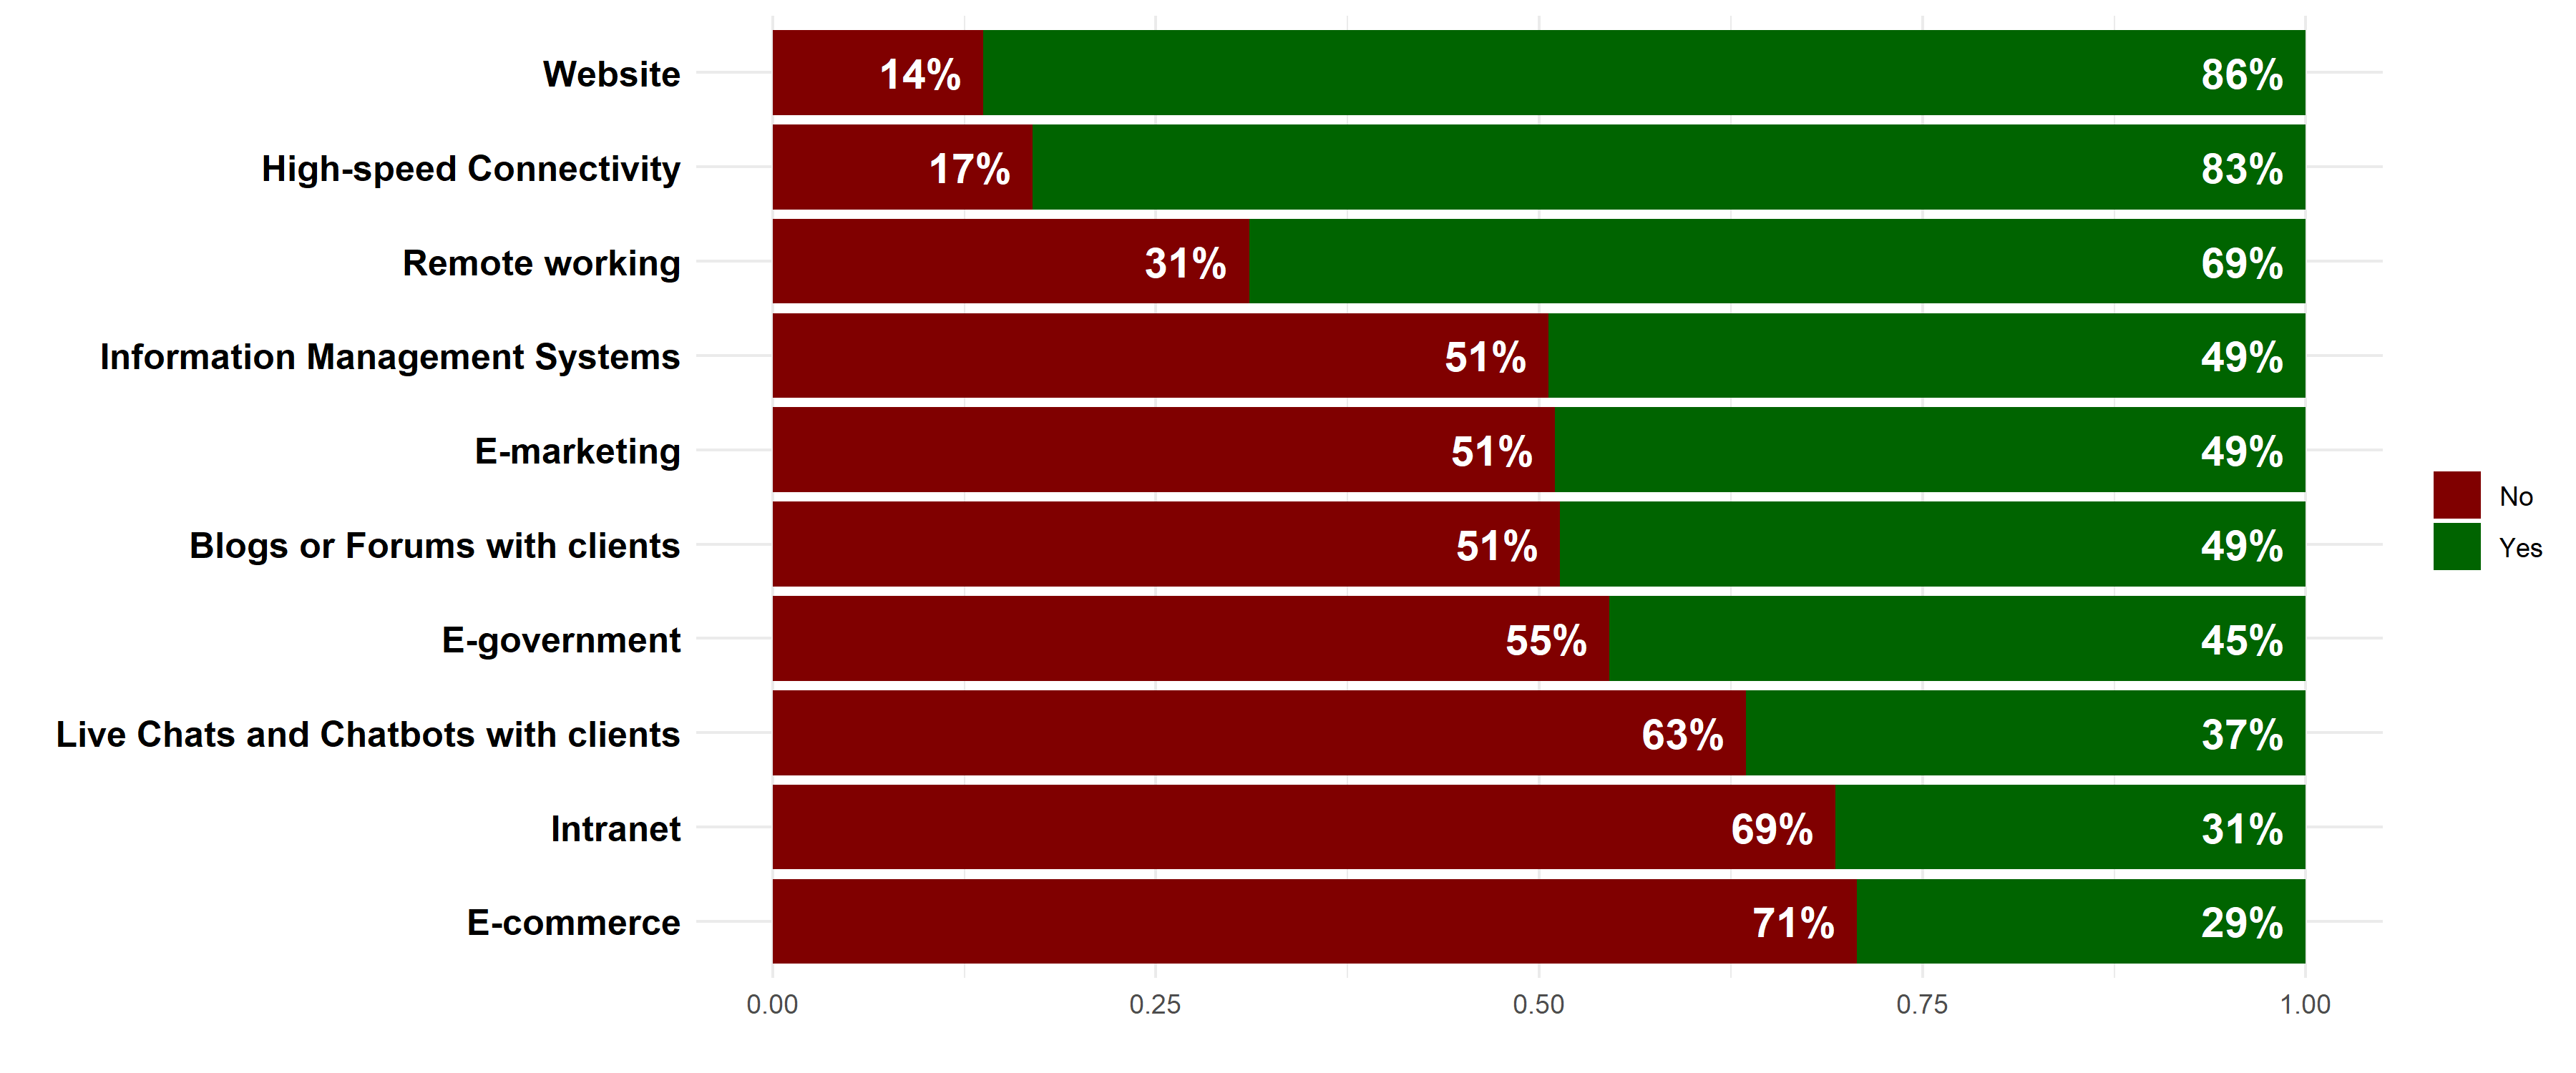
\includegraphics[width=\textwidth]{../Output/q3.png}

        \end{figure}
    \end{frame}

    \begin{frame}{DMA - Question 4}
        \centering\textit{Which of the following advanced digital technologies are already used by your enterprise?}
        \begin{figure}
            \centering
            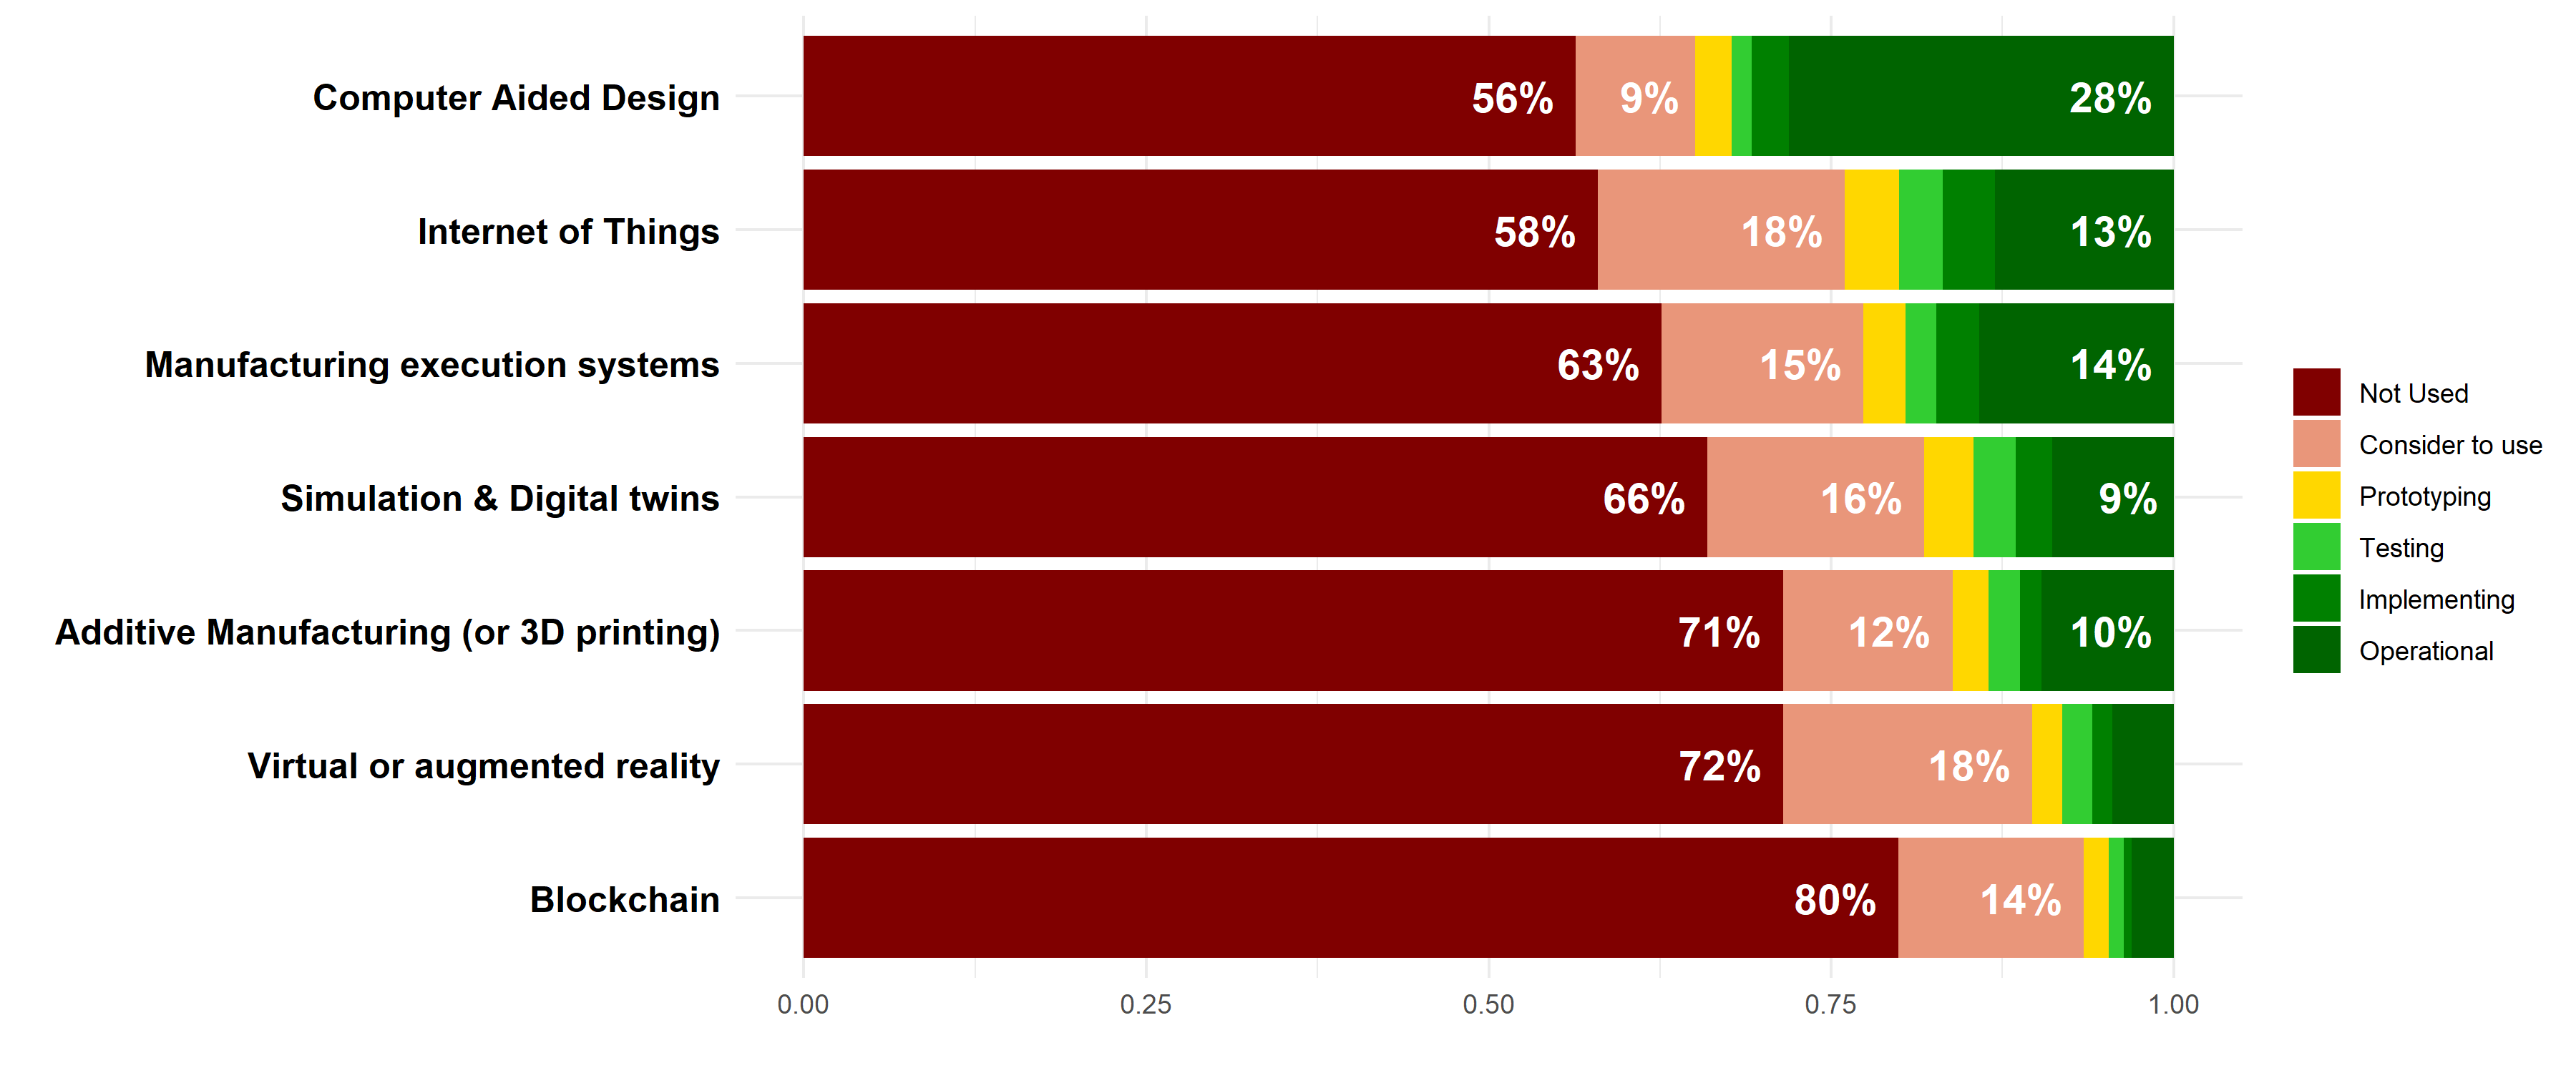
\includegraphics[width=\textwidth]{../Output/q4.png}

        \end{figure}
    \end{frame}

    \begin{frame}{DMA - Question 5}
        \centering\textit{What does your enterprise do to re-skill and up-skill its staff for digitalisation?}
        \begin{figure}
            \centering
            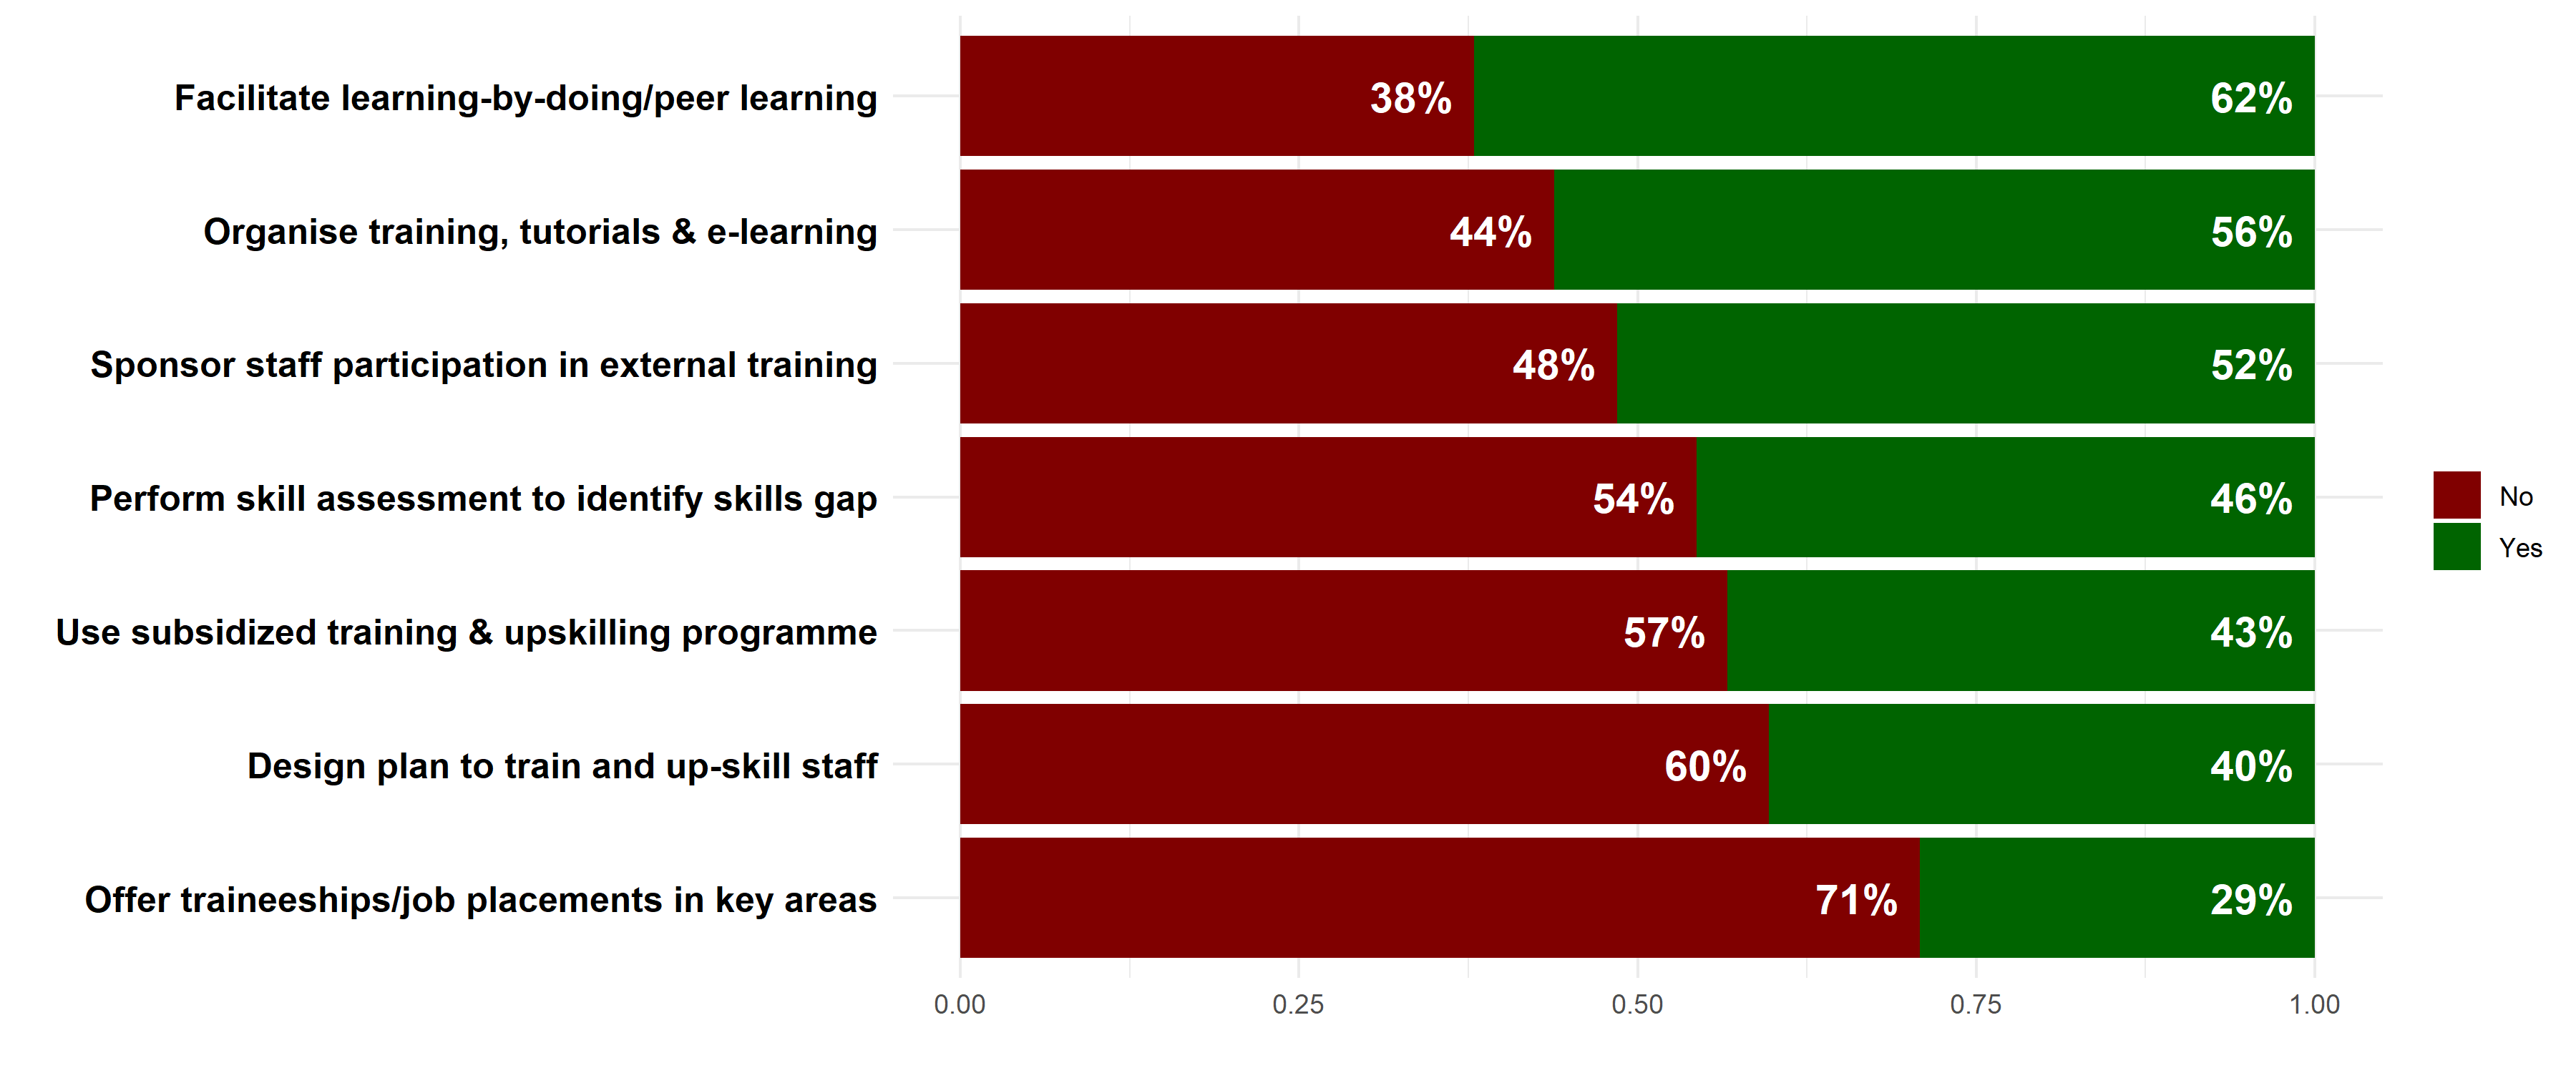
\includegraphics[width=\textwidth]{../Output/q5.png}

        \end{figure}
    \end{frame}

    \begin{frame}{DMA - Question 6}
        \centering\textit{When adopting new digital solutions, how does your enterprise engage and empower its staff?}
        \begin{figure}
            \centering
            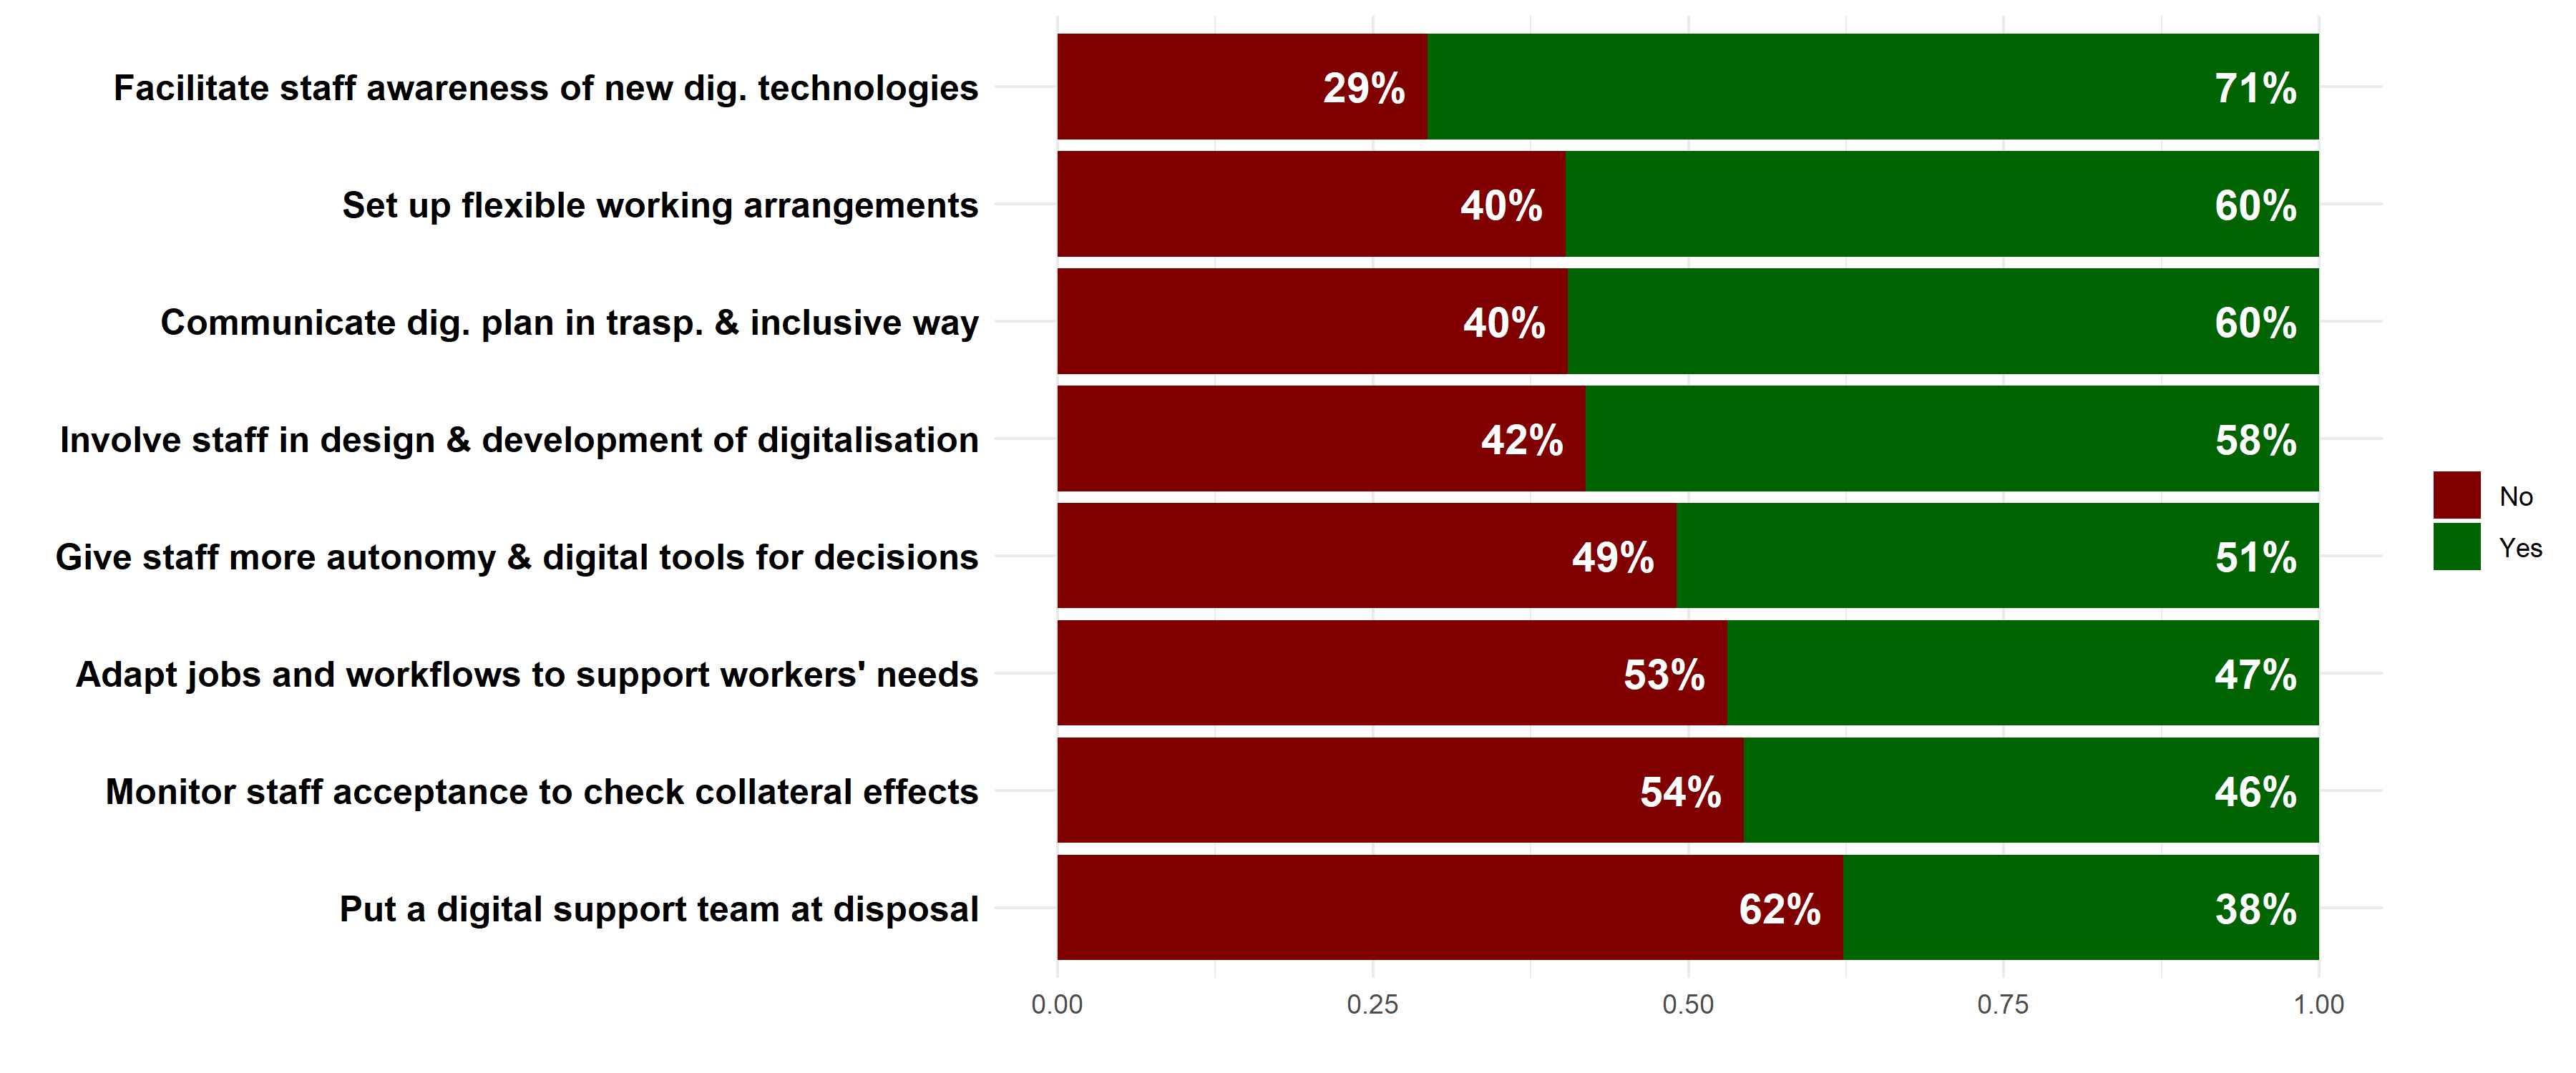
\includegraphics[width=\textwidth]{../Output/q6.png}

        \end{figure}
    \end{frame}

    \begin{frame}{DMA - Question 7}
        \centering\textit{How is your enterprise data managed (i.e. stored, organised, accessed and exploited)?}
        \begin{figure}
            \centering
            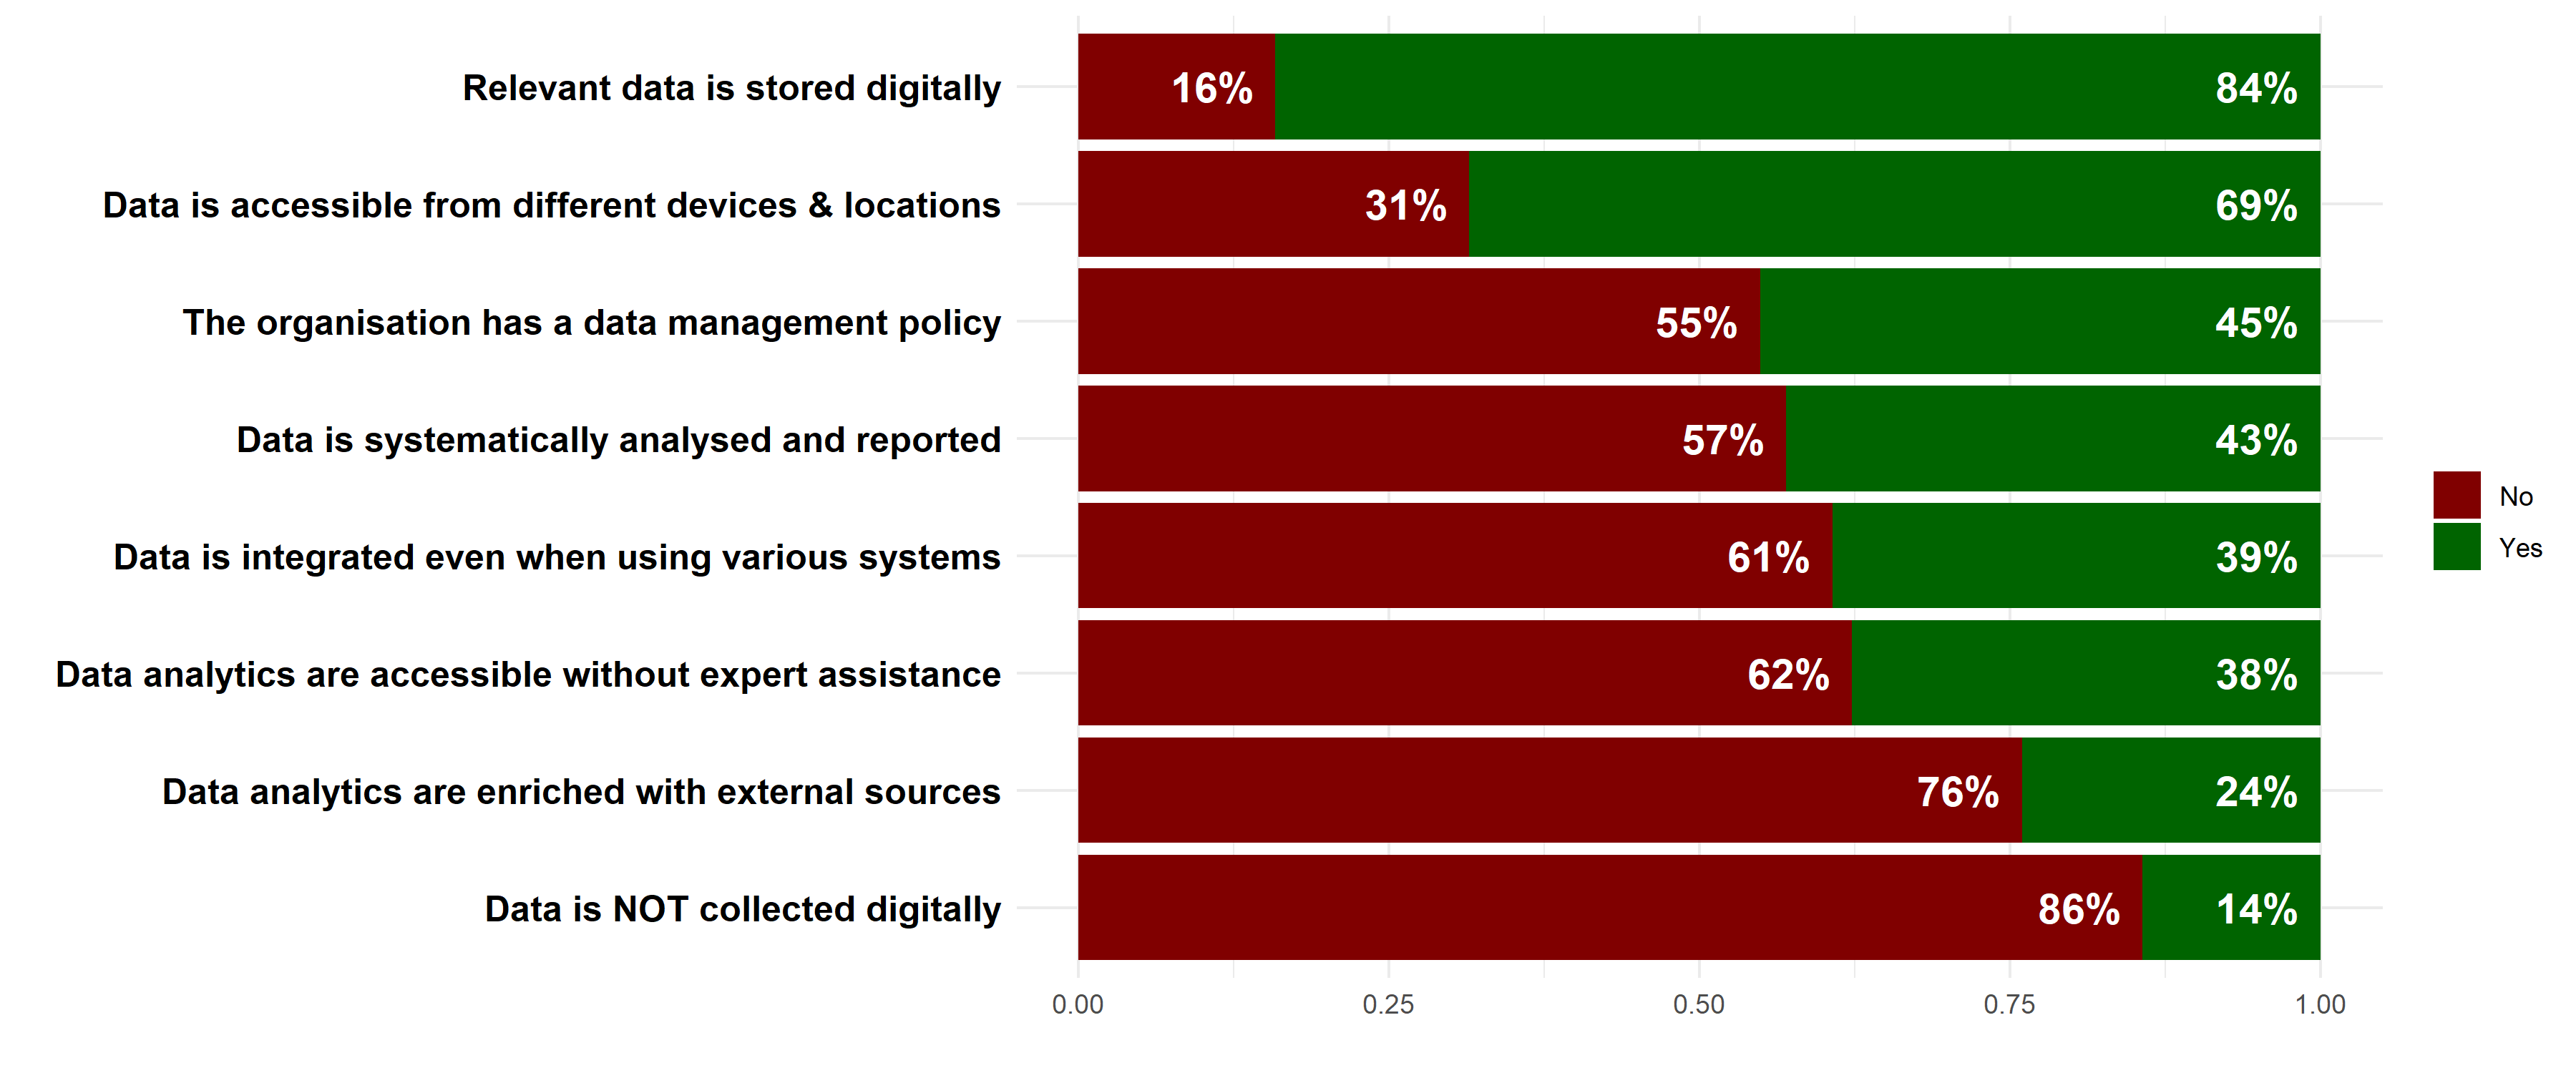
\includegraphics[width=\textwidth]{../Output/q7.png}

        \end{figure}
    \end{frame}

    \begin{frame}{DMA - Question 8}
        \centering\textit{Is your enterprise’s data sufficiently secured?}
        \begin{figure}
            \centering
            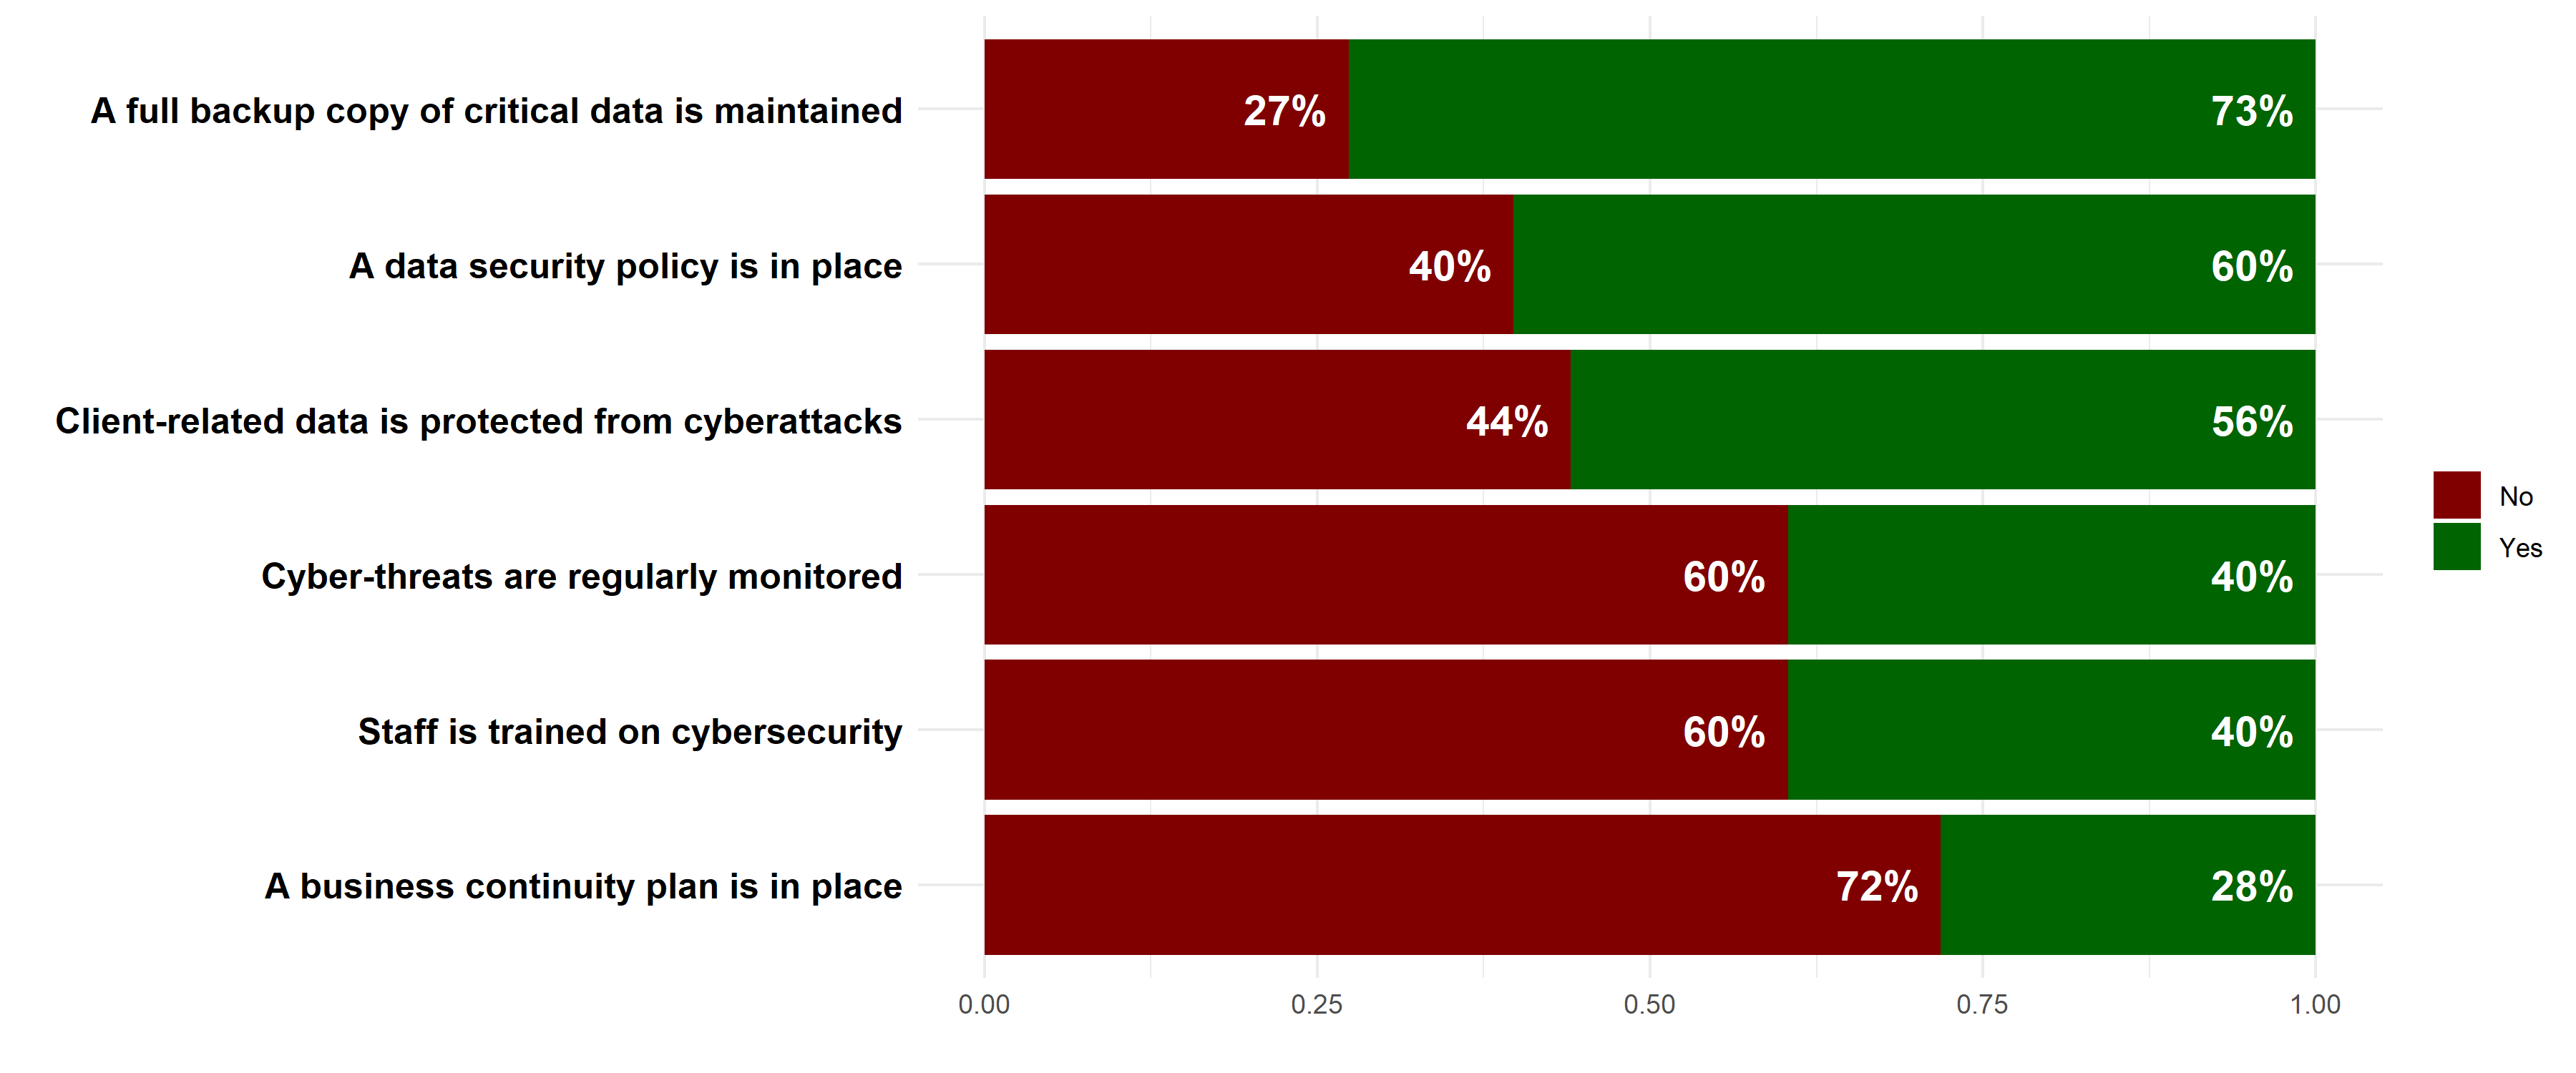
\includegraphics[width=\textwidth]{../Output/q8.png}

        \end{figure}
    \end{frame}

    \begin{frame}{DMA - Question 9}
        \centering\textit{Which of the following technologies and business applications are your enterprise already
        using?}
        \begin{figure}
            \centering
            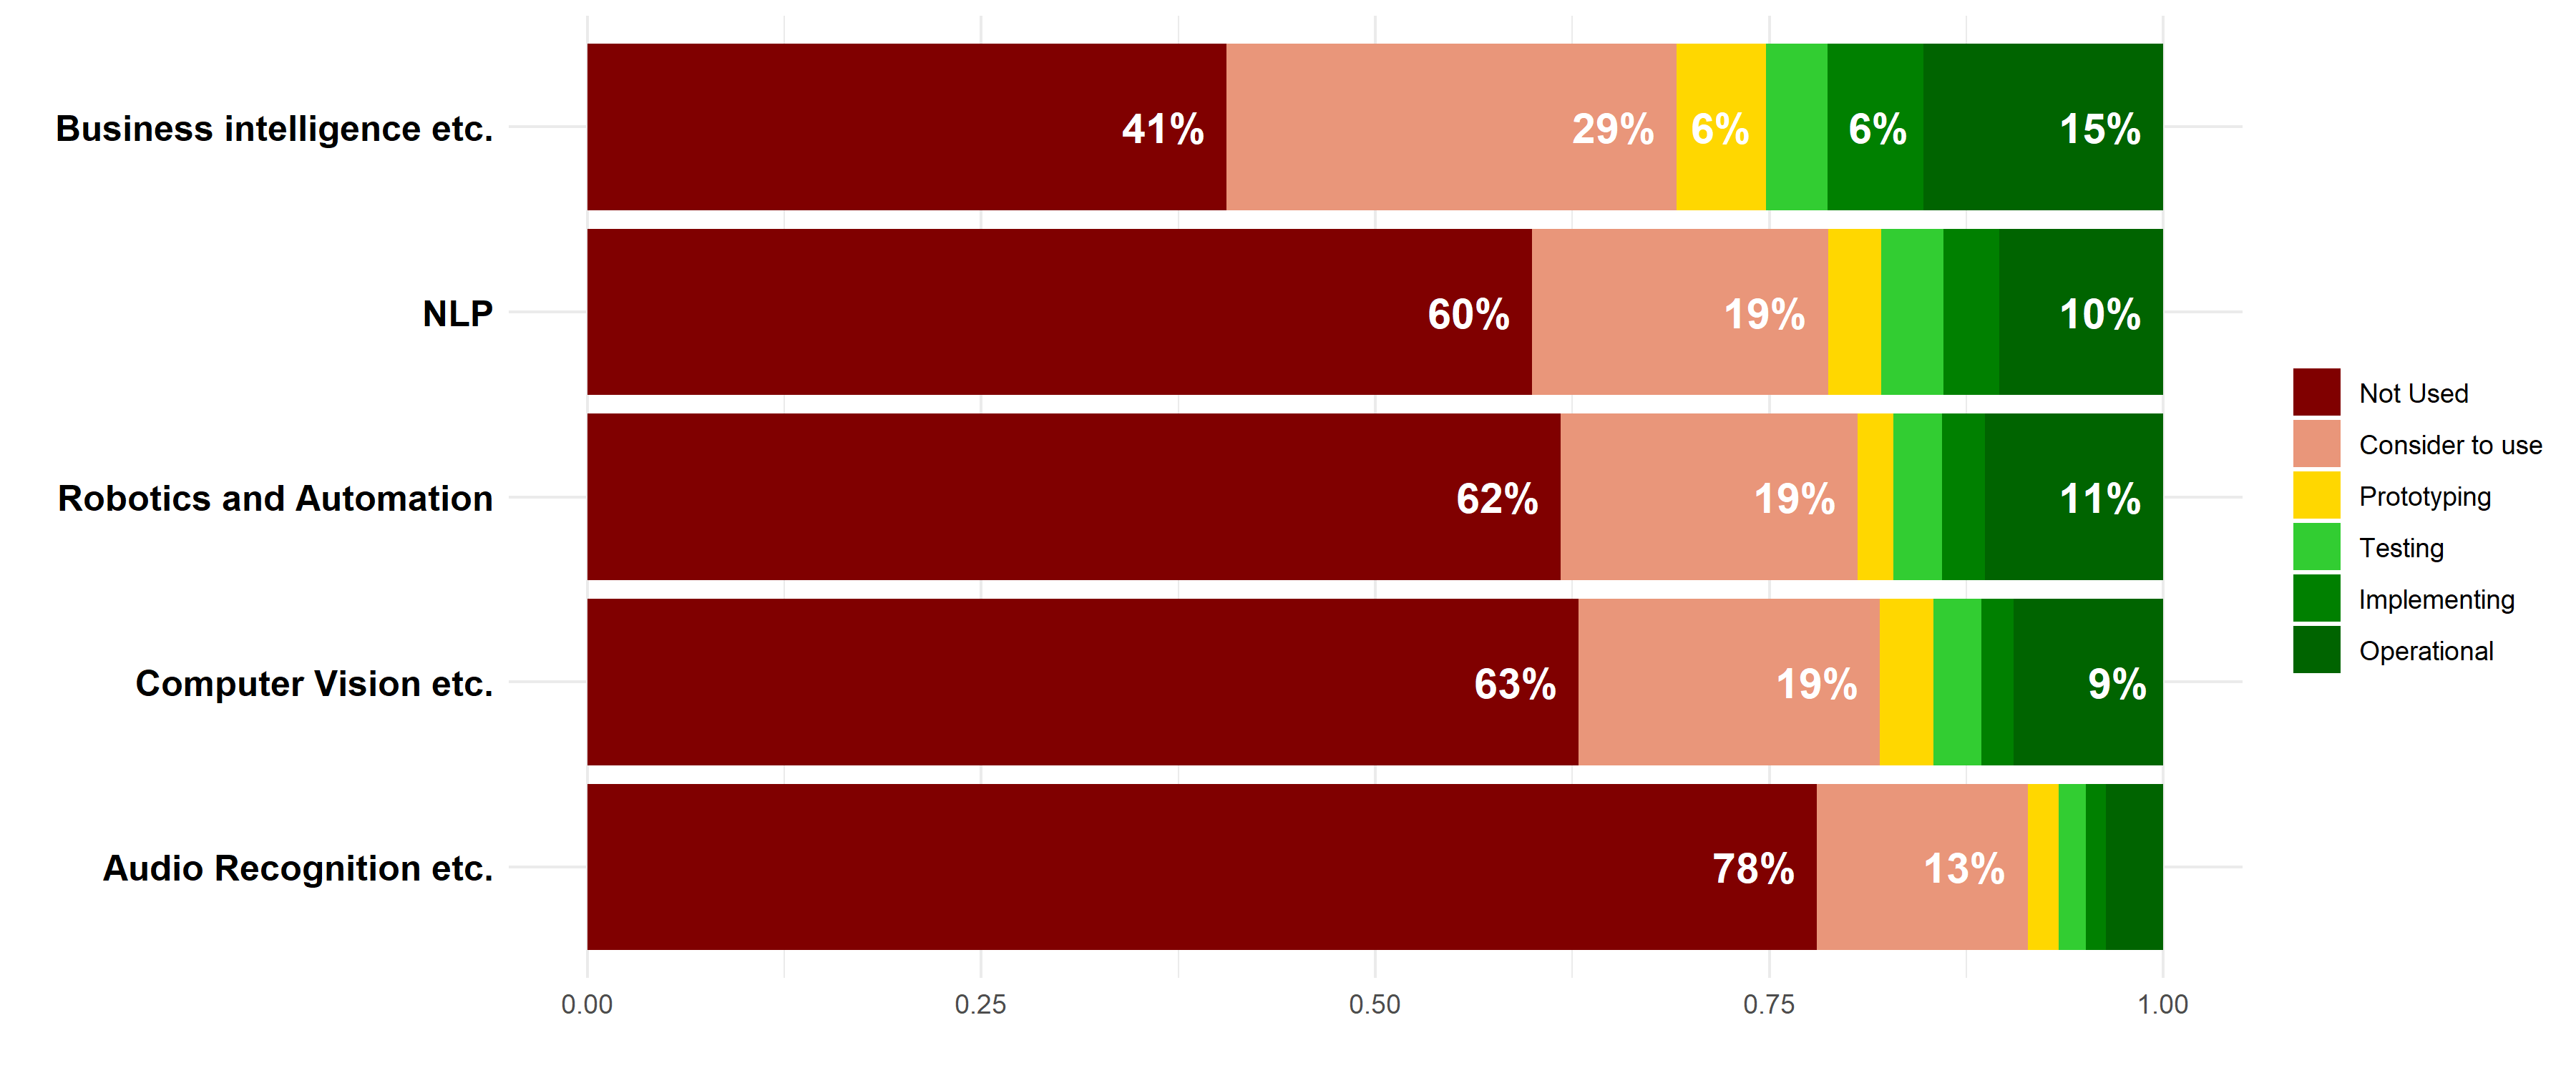
\includegraphics[width=\textwidth]{../Output/q9.png}

        \end{figure}
    \end{frame}

    \begin{frame}{DMA - Question 10}
        \centering\textit{How does your enterprise make use of digital technologies to contribute to environmental sustainability?}
        \begin{figure}
            \centering
            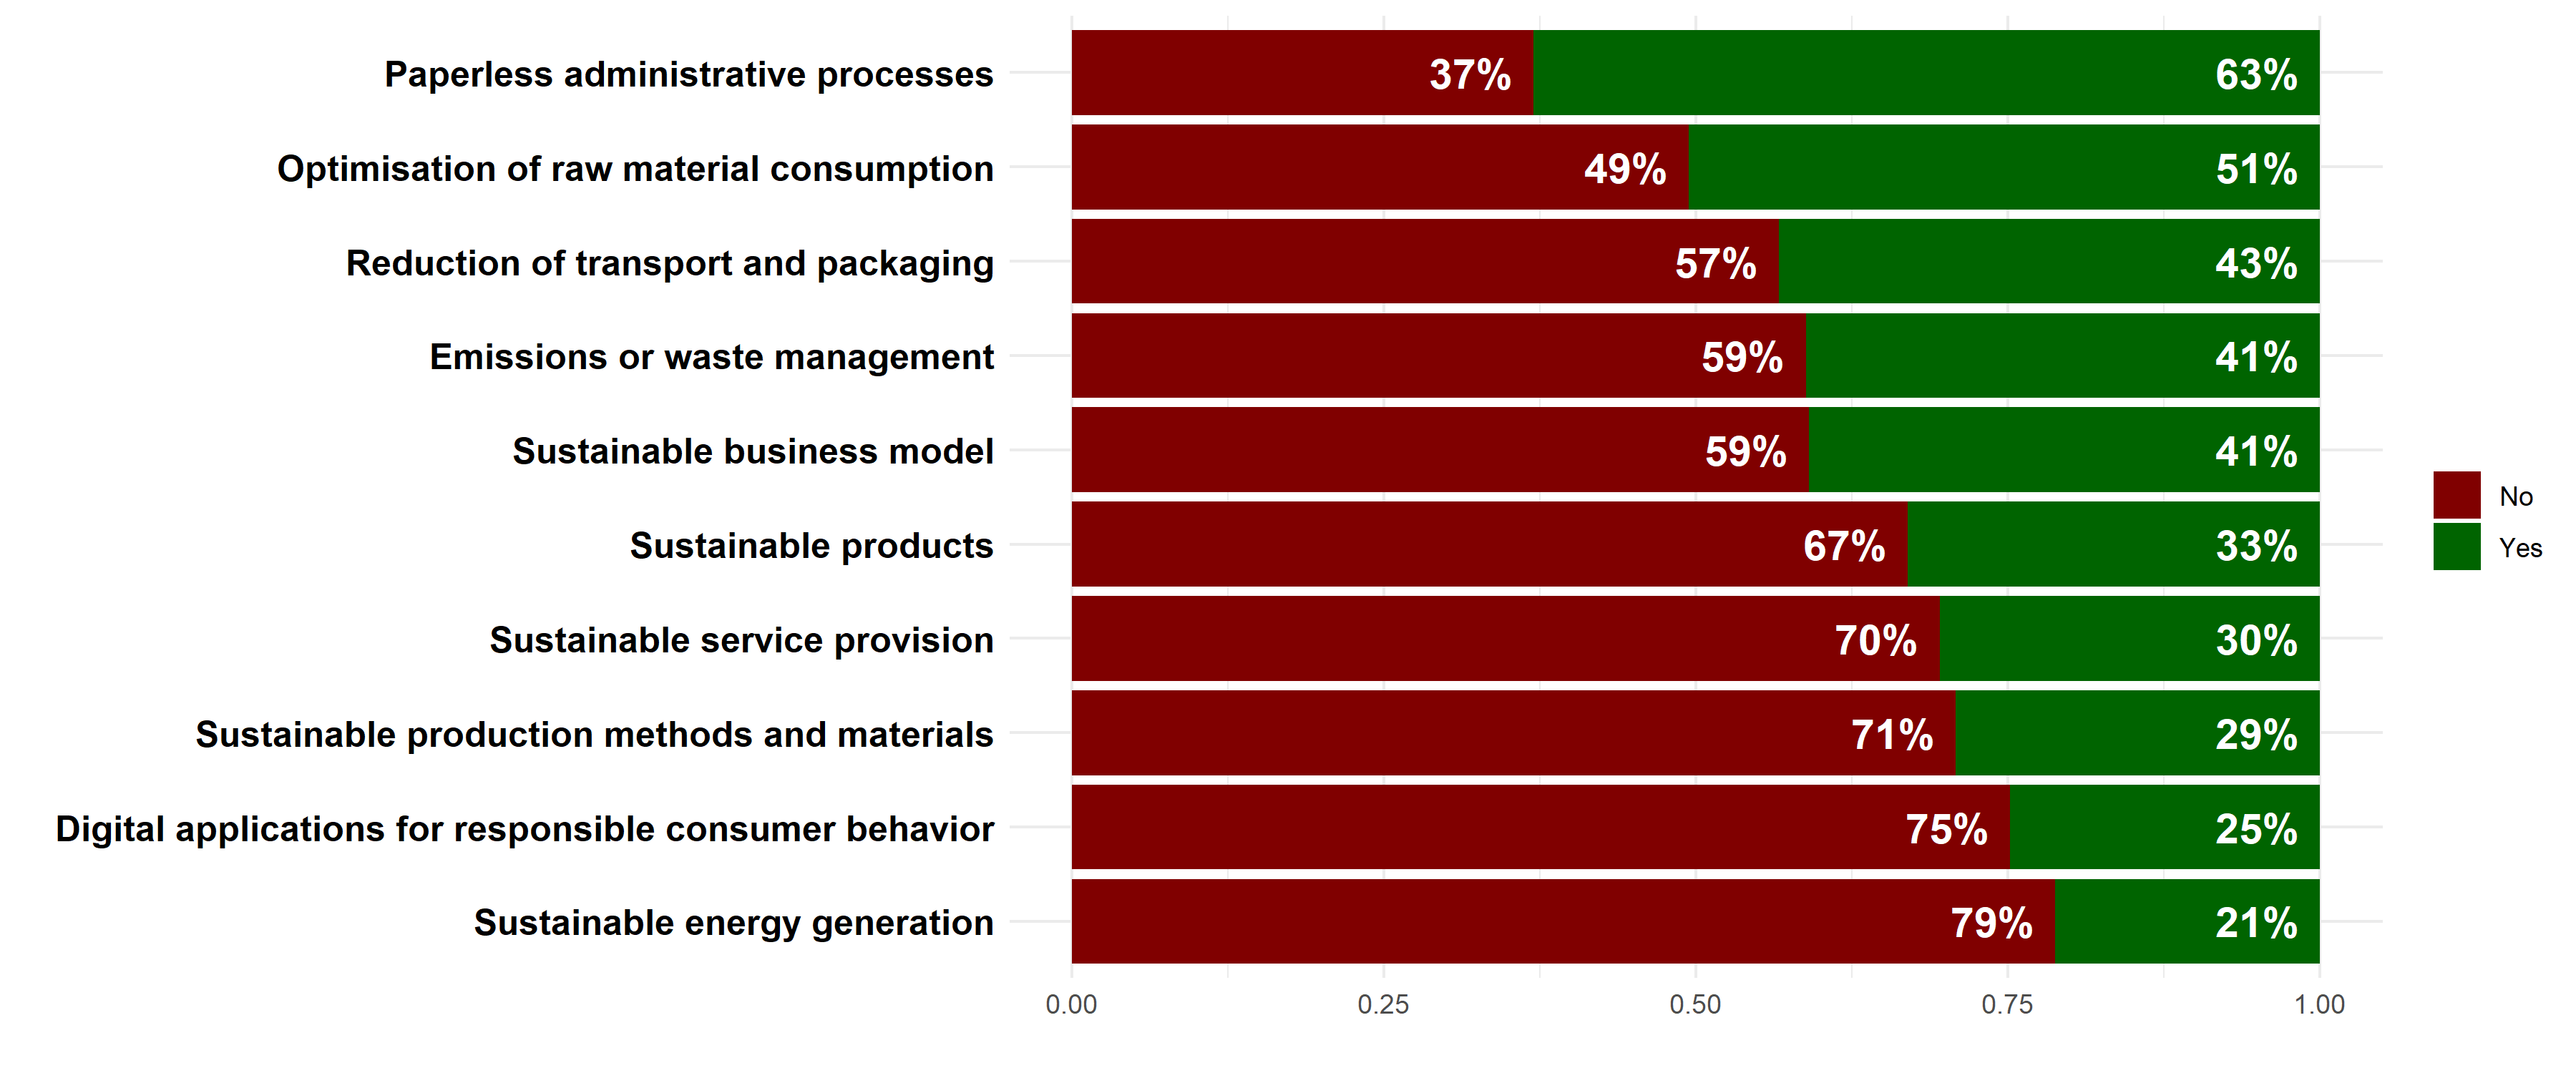
\includegraphics[width=\textwidth]{../Output/q10.png}

        \end{figure}
    \end{frame}

    \begin{frame}{DMA - Question 11}
        \centering\textit{Is your enterprise taking into account environmental impacts in its digital choices and practices?}
        \begin{figure}
            \centering
            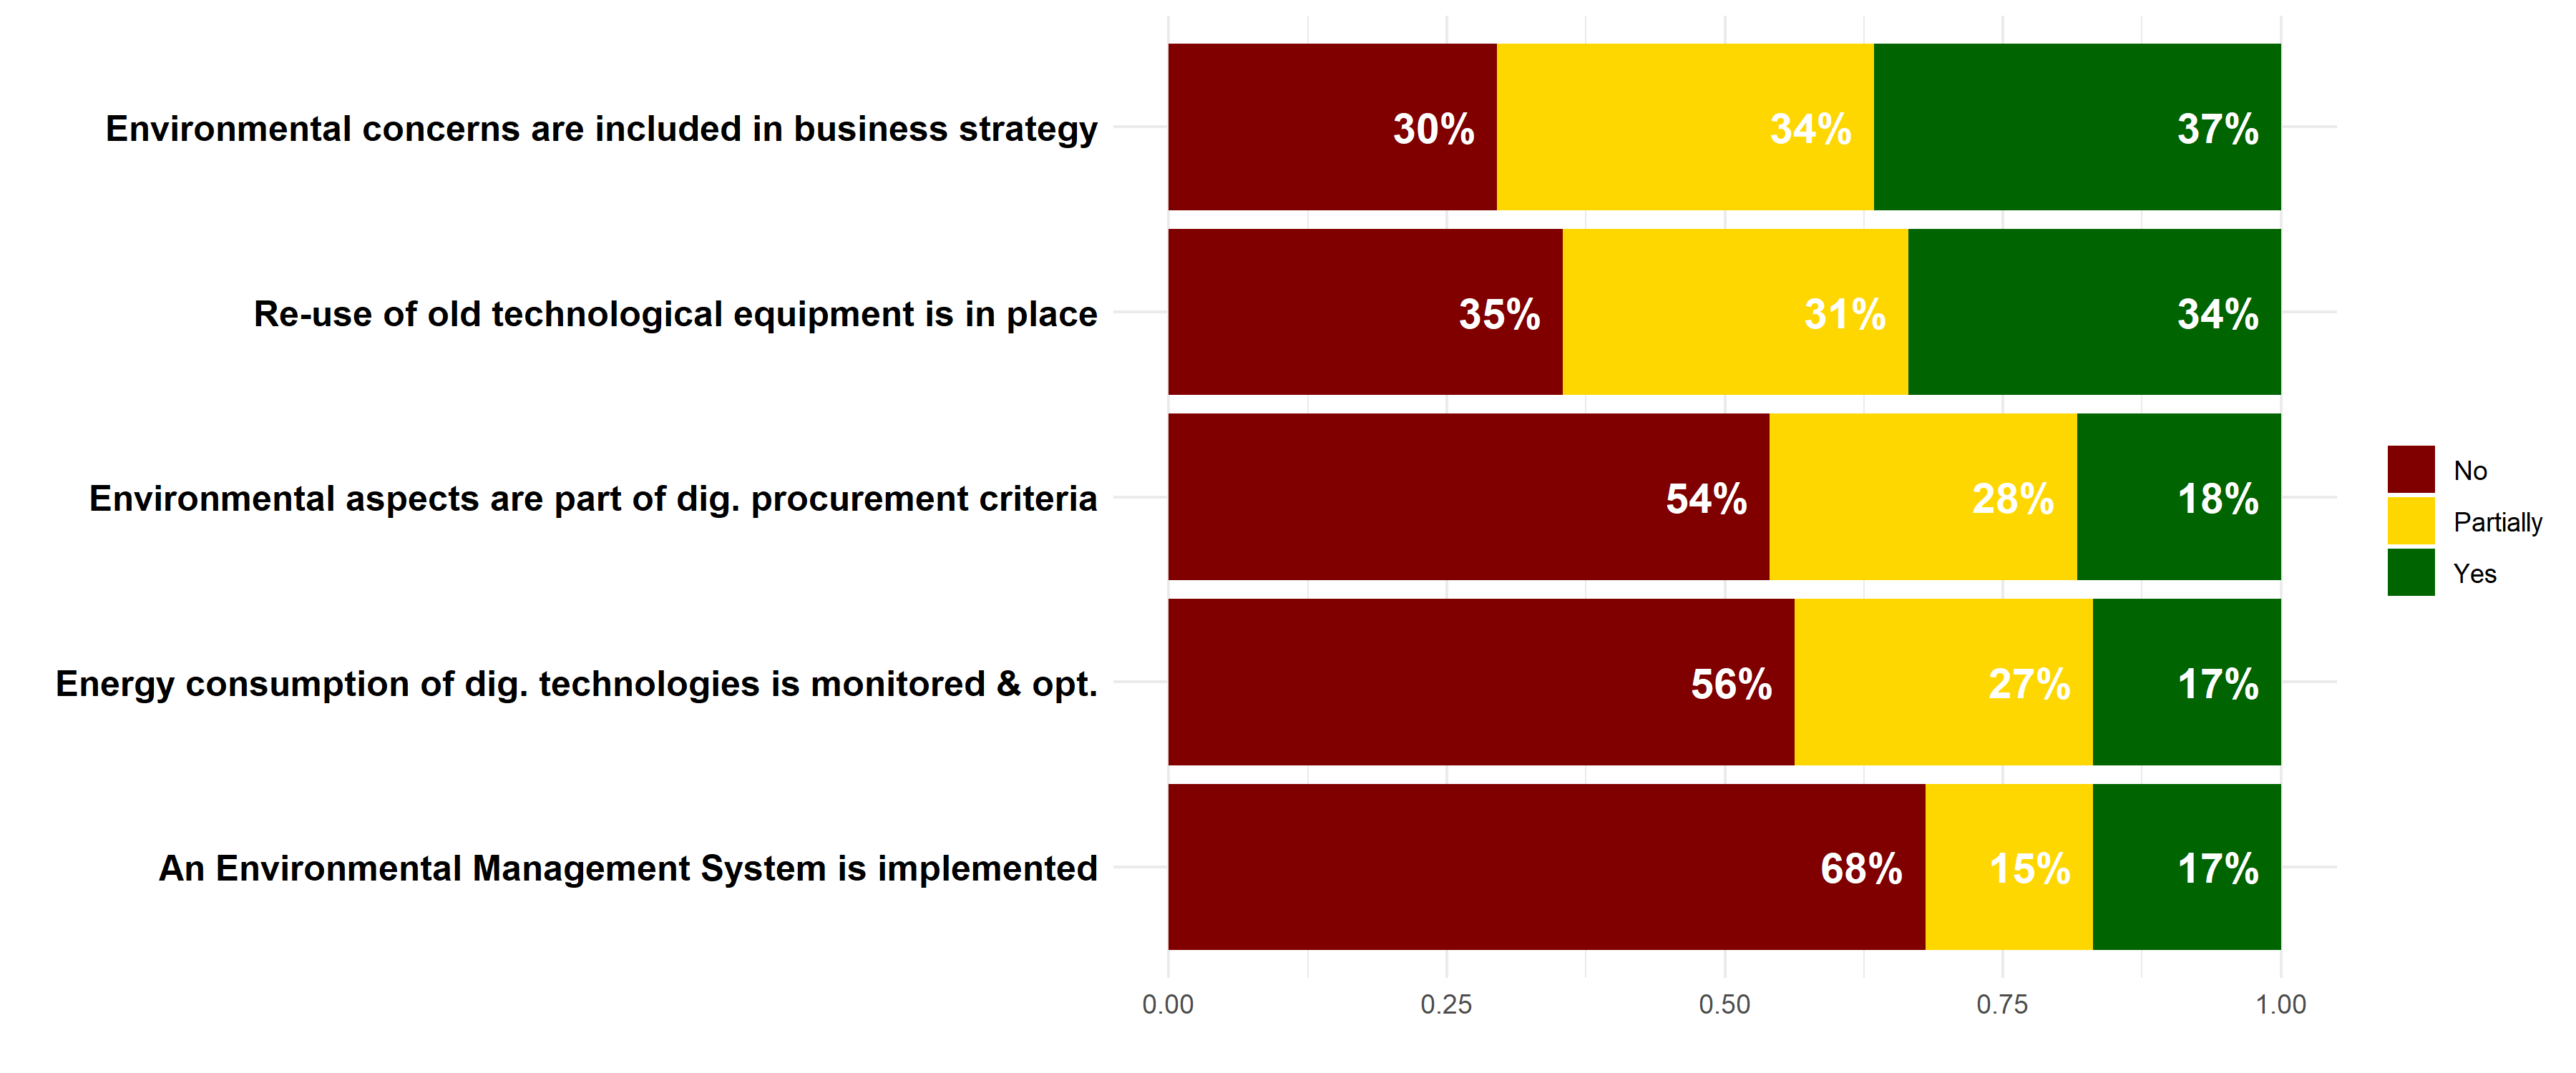
\includegraphics[width=\textwidth]{../Output/q11.png}
        \end{figure}
    \end{frame}
    
    \begin{frame}{DMA - Correlation Matrix of Dimensions}
        \begin{figure}
        \centering
        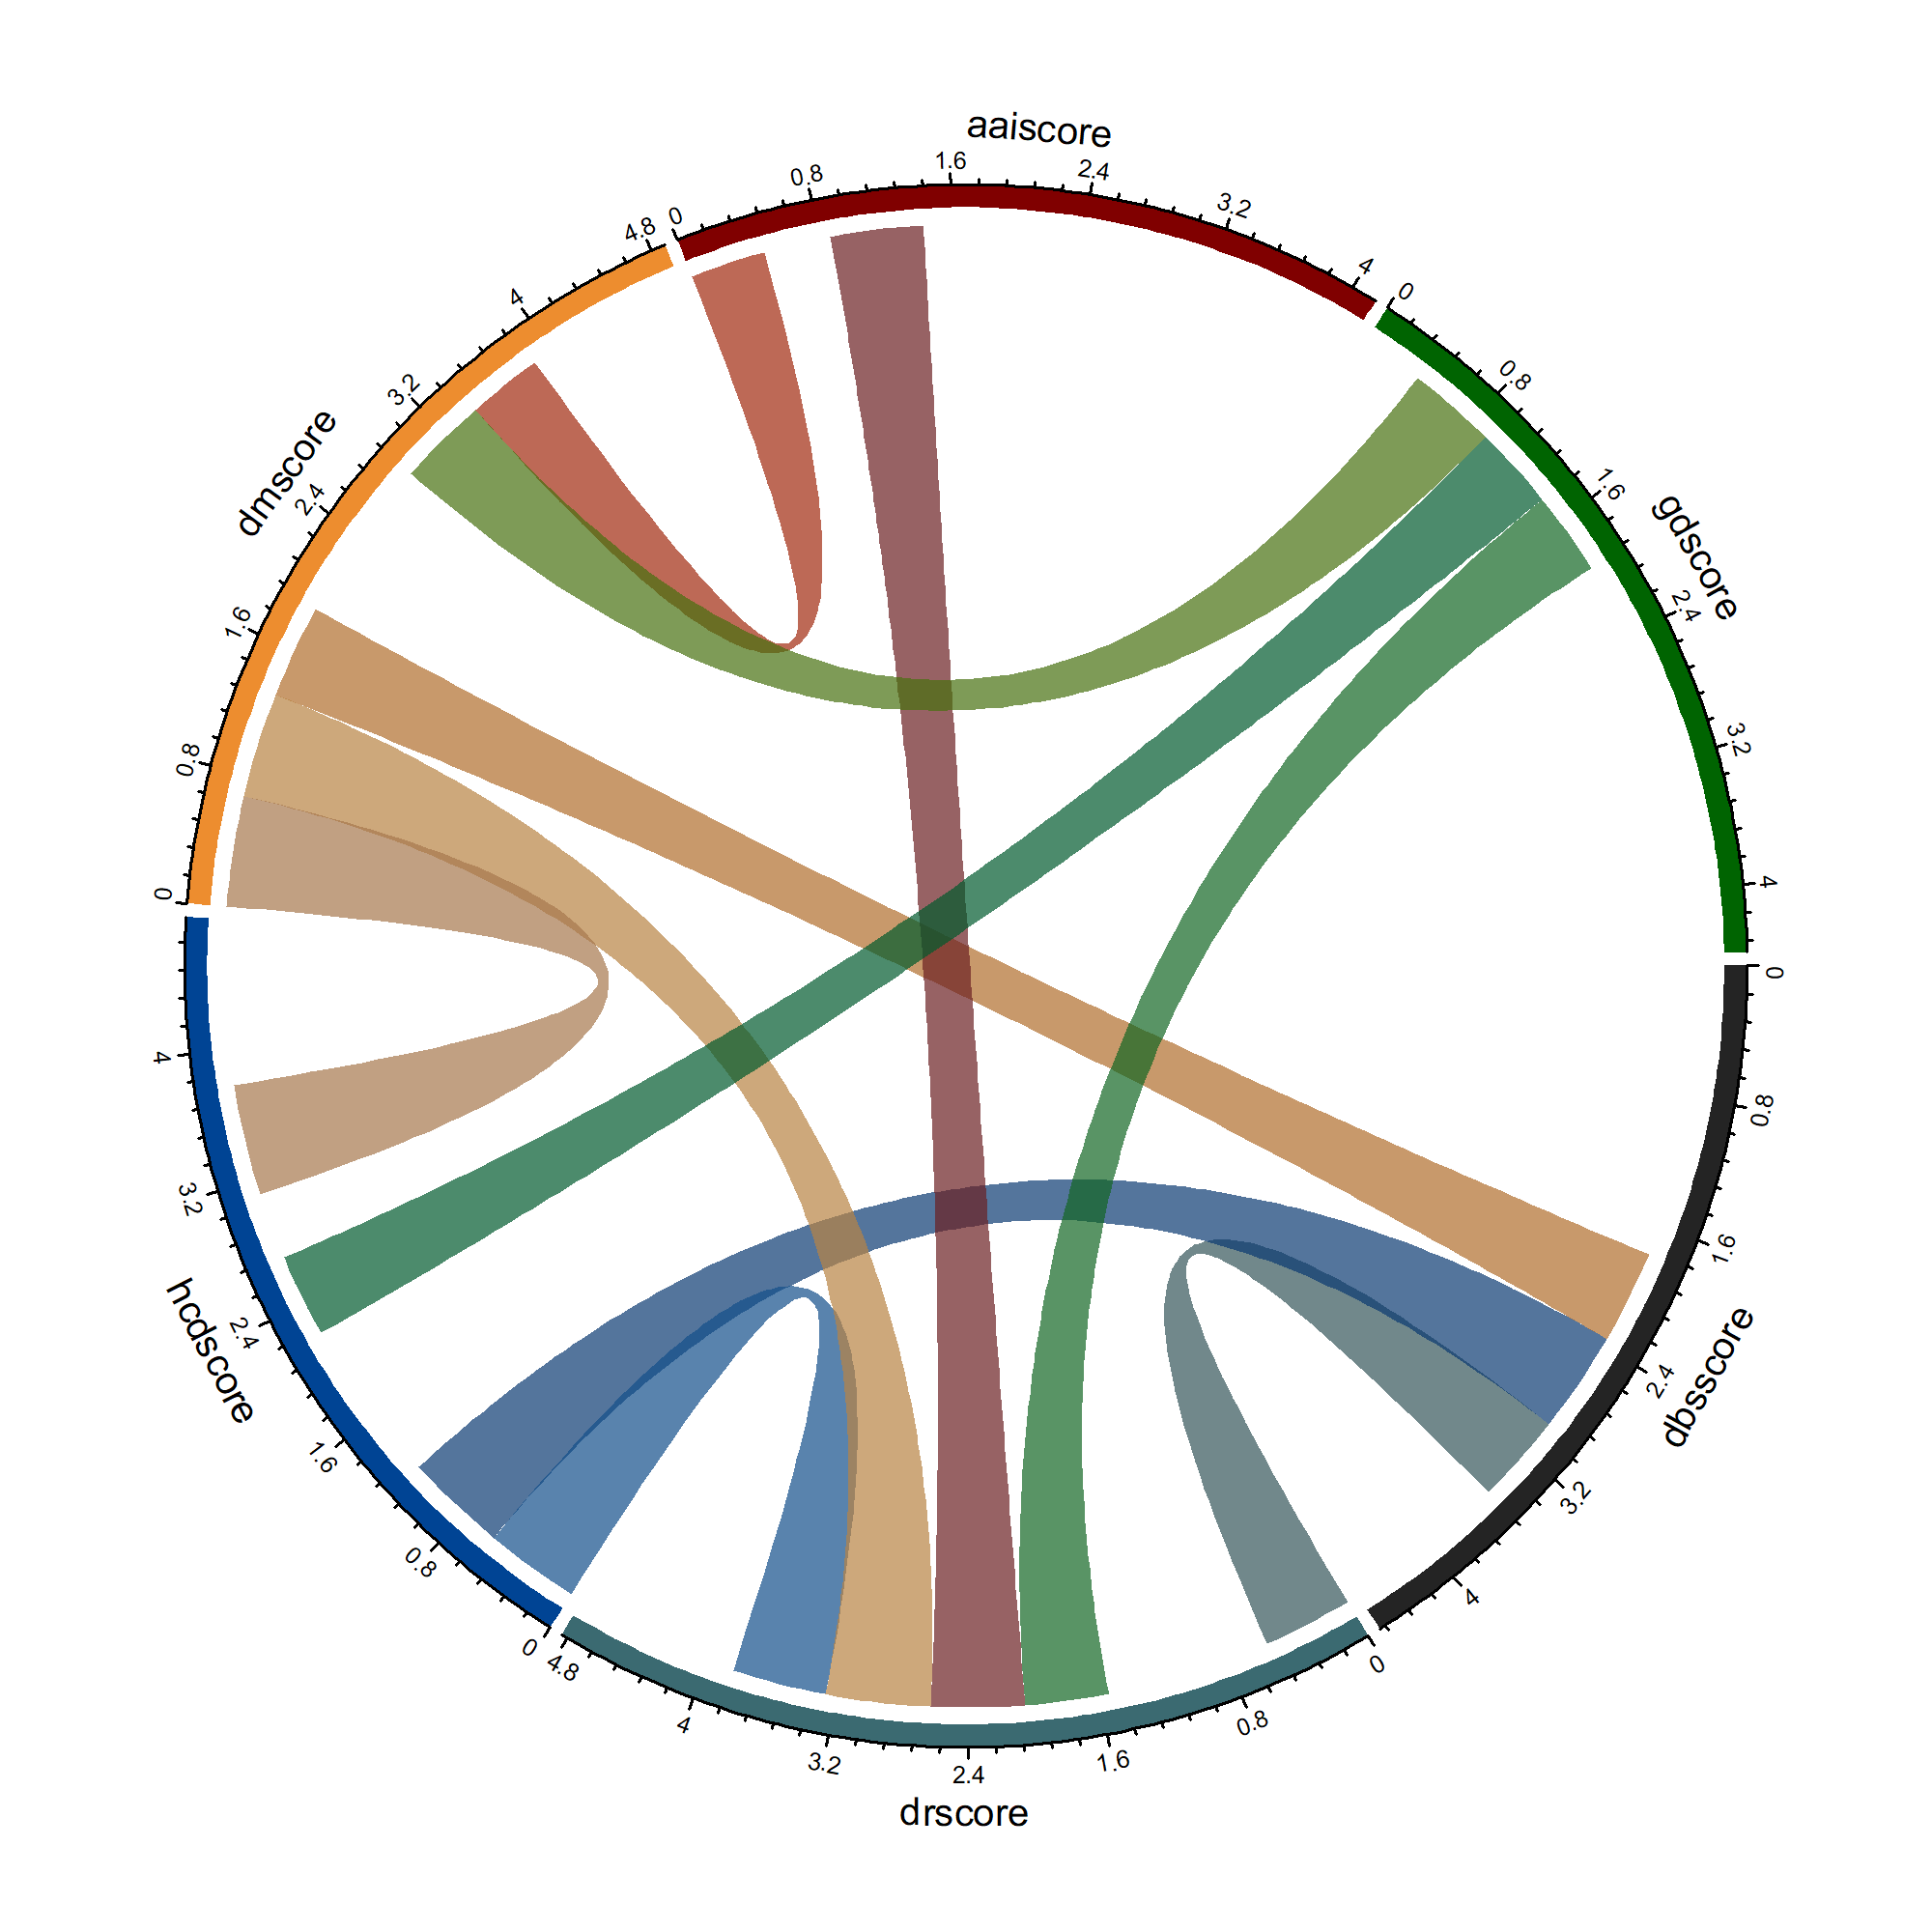
\includegraphics[width=0.7\textwidth]{../Output/theverysmallcorrmatrix_plot.png}
    \end{figure}
    \end{frame}

    \begin{frame}{DMA - Correlation Matrix of Subdimensions}
        \begin{figure}
        \centering
        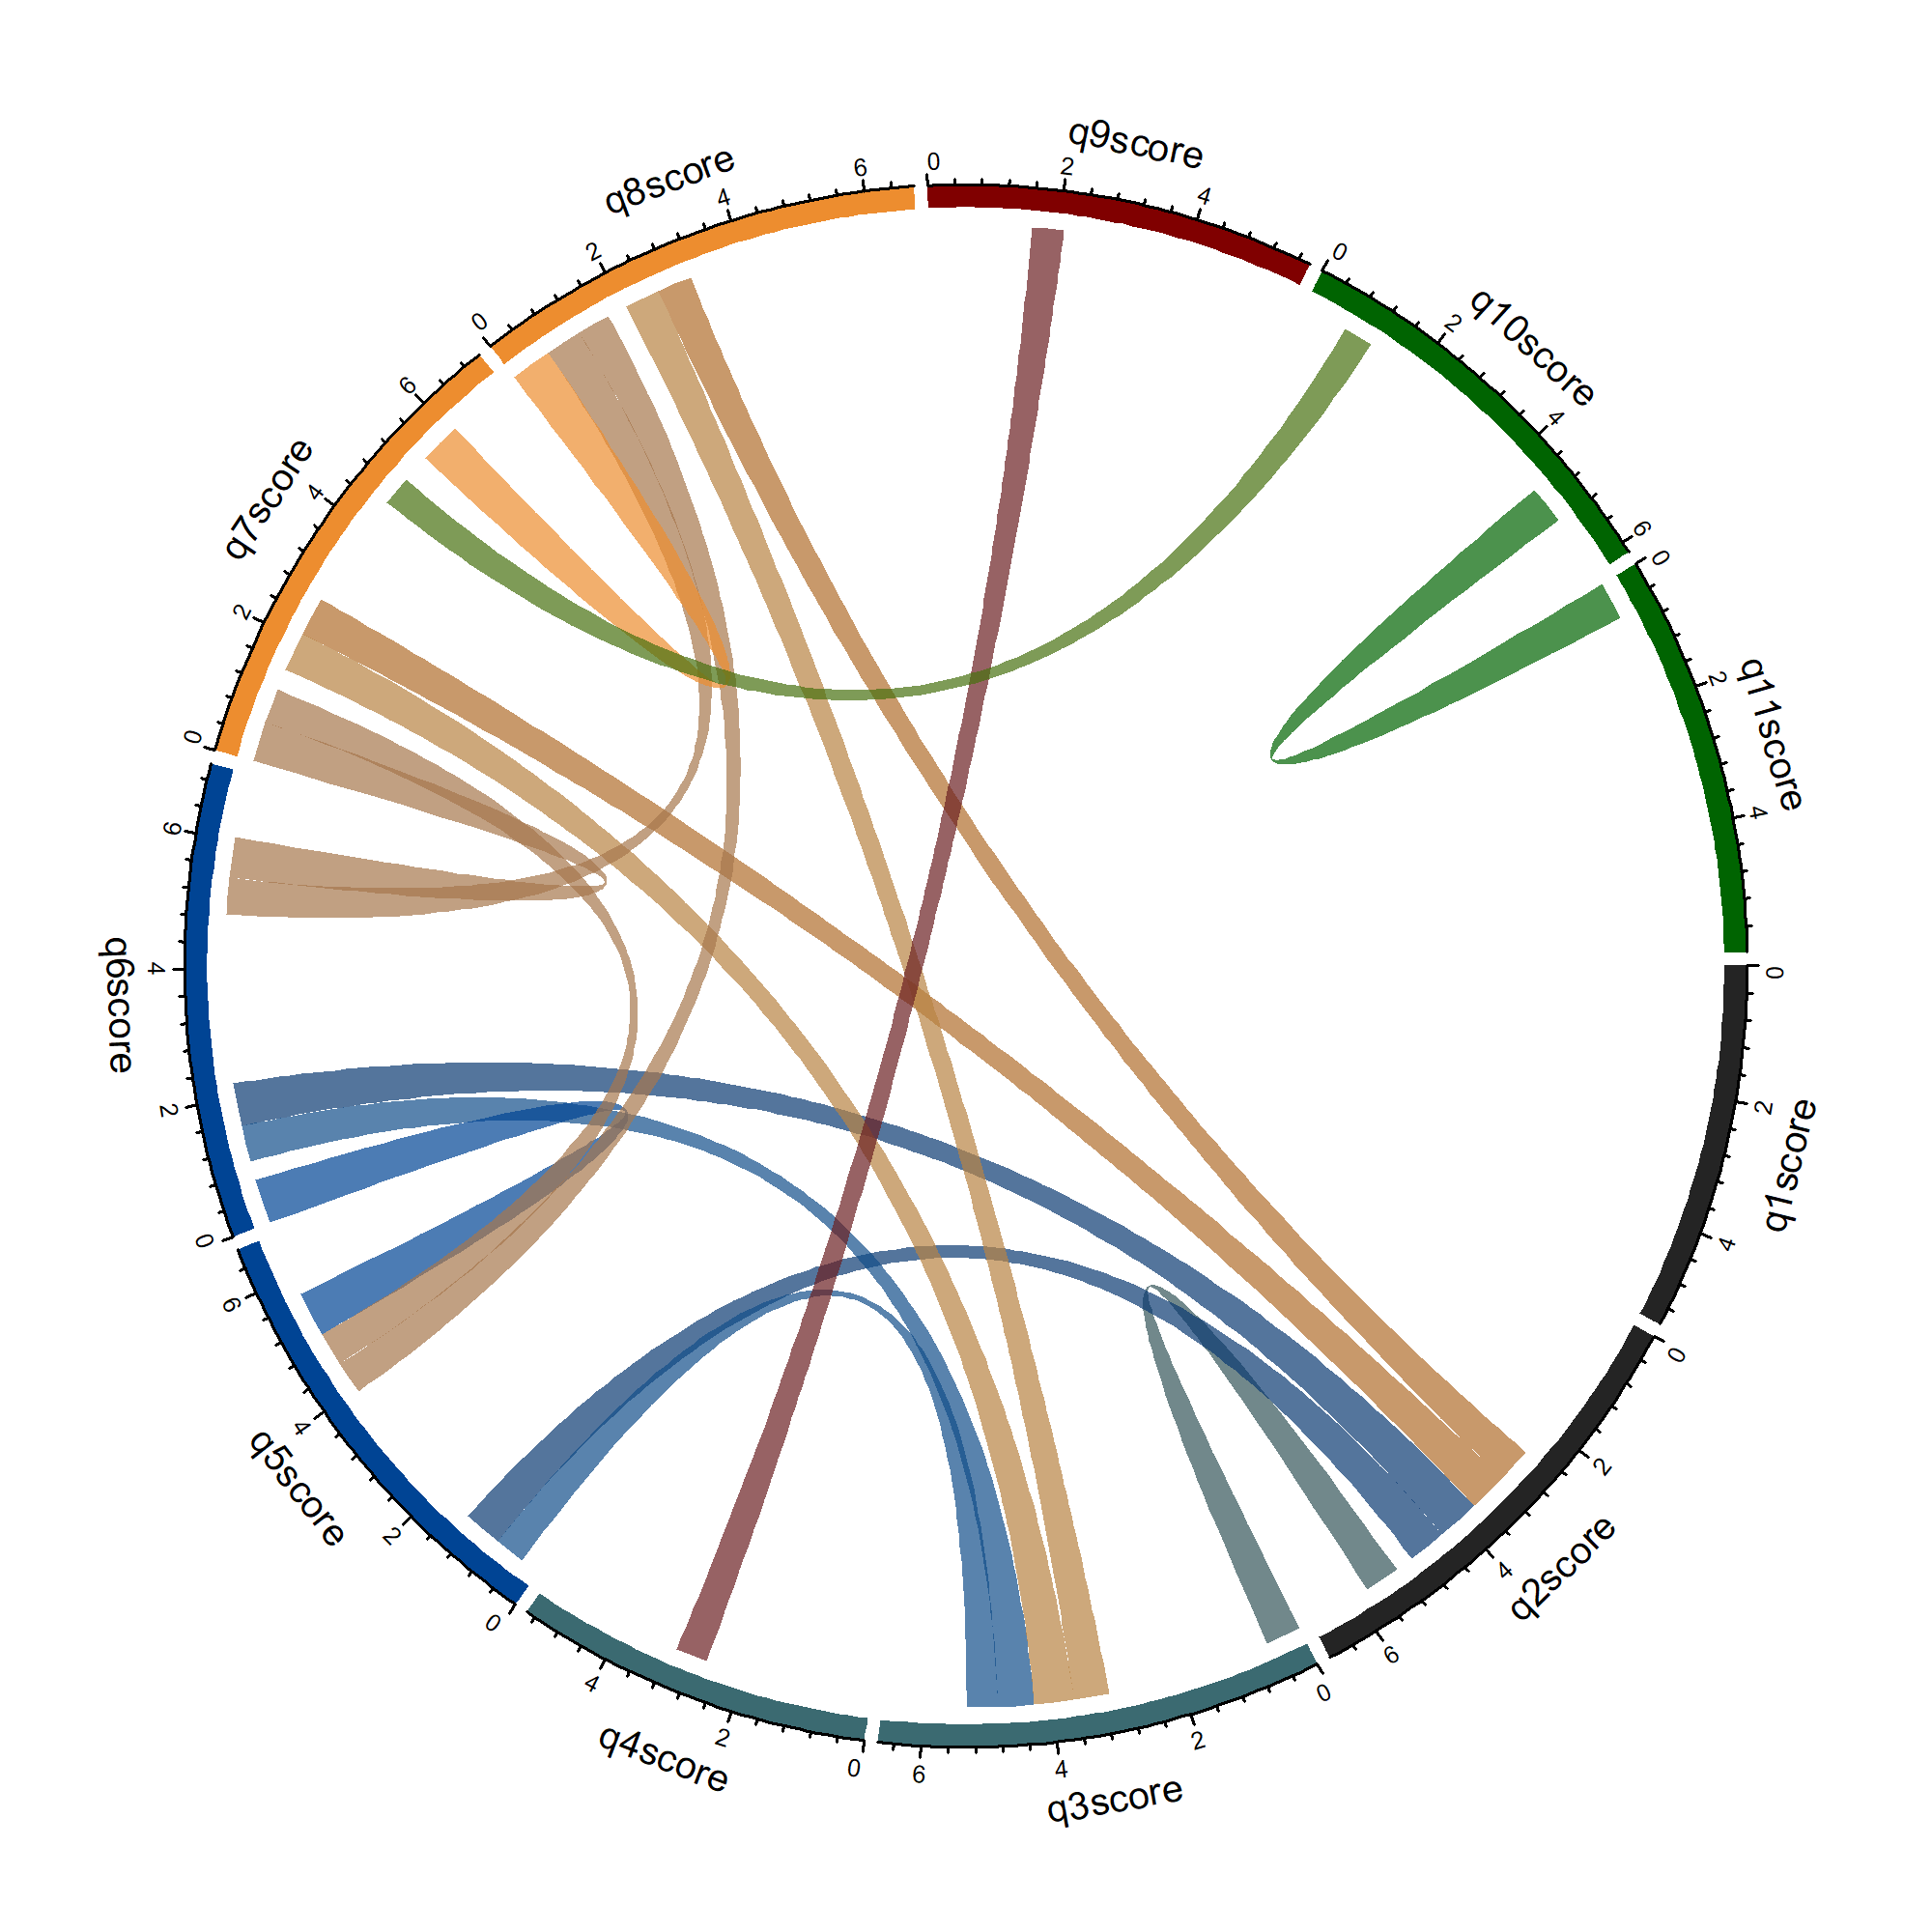
\includegraphics[width=0.7\textwidth]{../Output/thesmallcorrmatrix_plot.png}
    \end{figure}
    \end{frame}

    \begin{frame}{DMA - Network of Question Items}
        \begin{figure}
            \centering
            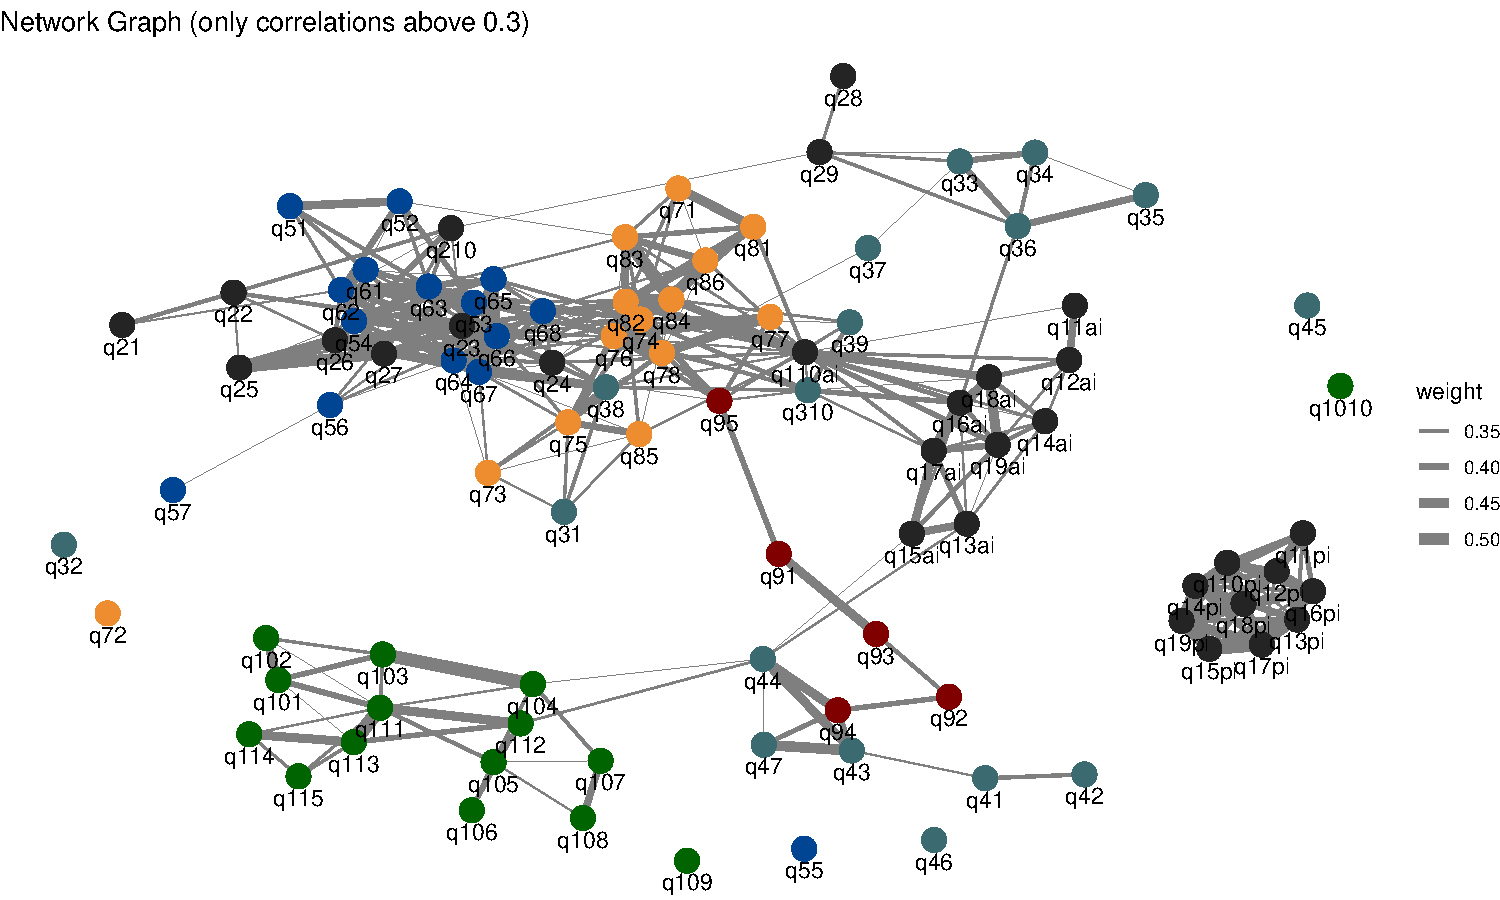
\includegraphics[width=\textwidth]{../Output/network_graph.pdf}
        \end{figure}
    \end{frame}

    \begin{frame}{Treated vs Control - Comparison Table}
        % latex table generated in R 4.4.2 by xtable 1.8-4 package
% Wed Apr  9 18:31:31 2025
\begin{table}[ht]
\centering
\begin{tabular}{lrrr}
  \hline
Statistic & Treated\_0 & Treated\_1 & p\_value \\ 
  \hline
N & 3643.00 & 1249.00 &  \\ 
  Mean\_Employees & 0.03 & 0.09 & 0.00 \\ 
  SD\_Employees & 0.17 & 0.37 &  \\ 
  Mean\_TotalAssets & 14.09 & 15.18 & 0.80 \\ 
  SD\_TotalAssets & 185.97 & 108.15 &  \\ 
  Mean\_LiquidityRatio & 4.15 & 2.33 & 0.00 \\ 
  SD\_LiquidityRatio & 8.41 & 2.90 &  \\ 
  Mean\_Solvency & 37.65 & 50.51 & 0.00 \\ 
  SD\_Solvency & 35.45 & 25.62 &  \\ 
  Mean\_turnover & 9.15 & 16.02 & 0.00 \\ 
  SD\_turnover & 70.39 & 74.00 &  \\ 
   \hline
\end{tabular}
\caption{Comparison between Control Firms (Treated = 0) and Treated ones (Treated = 1), with p-values for the t-test of equal means} 
\end{table}


    \end{frame}

    \begin{frame}{Treated vs Control - Distributions Compared}
        \begin{figure}[ht]
            \centering
            \begin{subfigure}[b]{0.45\textwidth}
                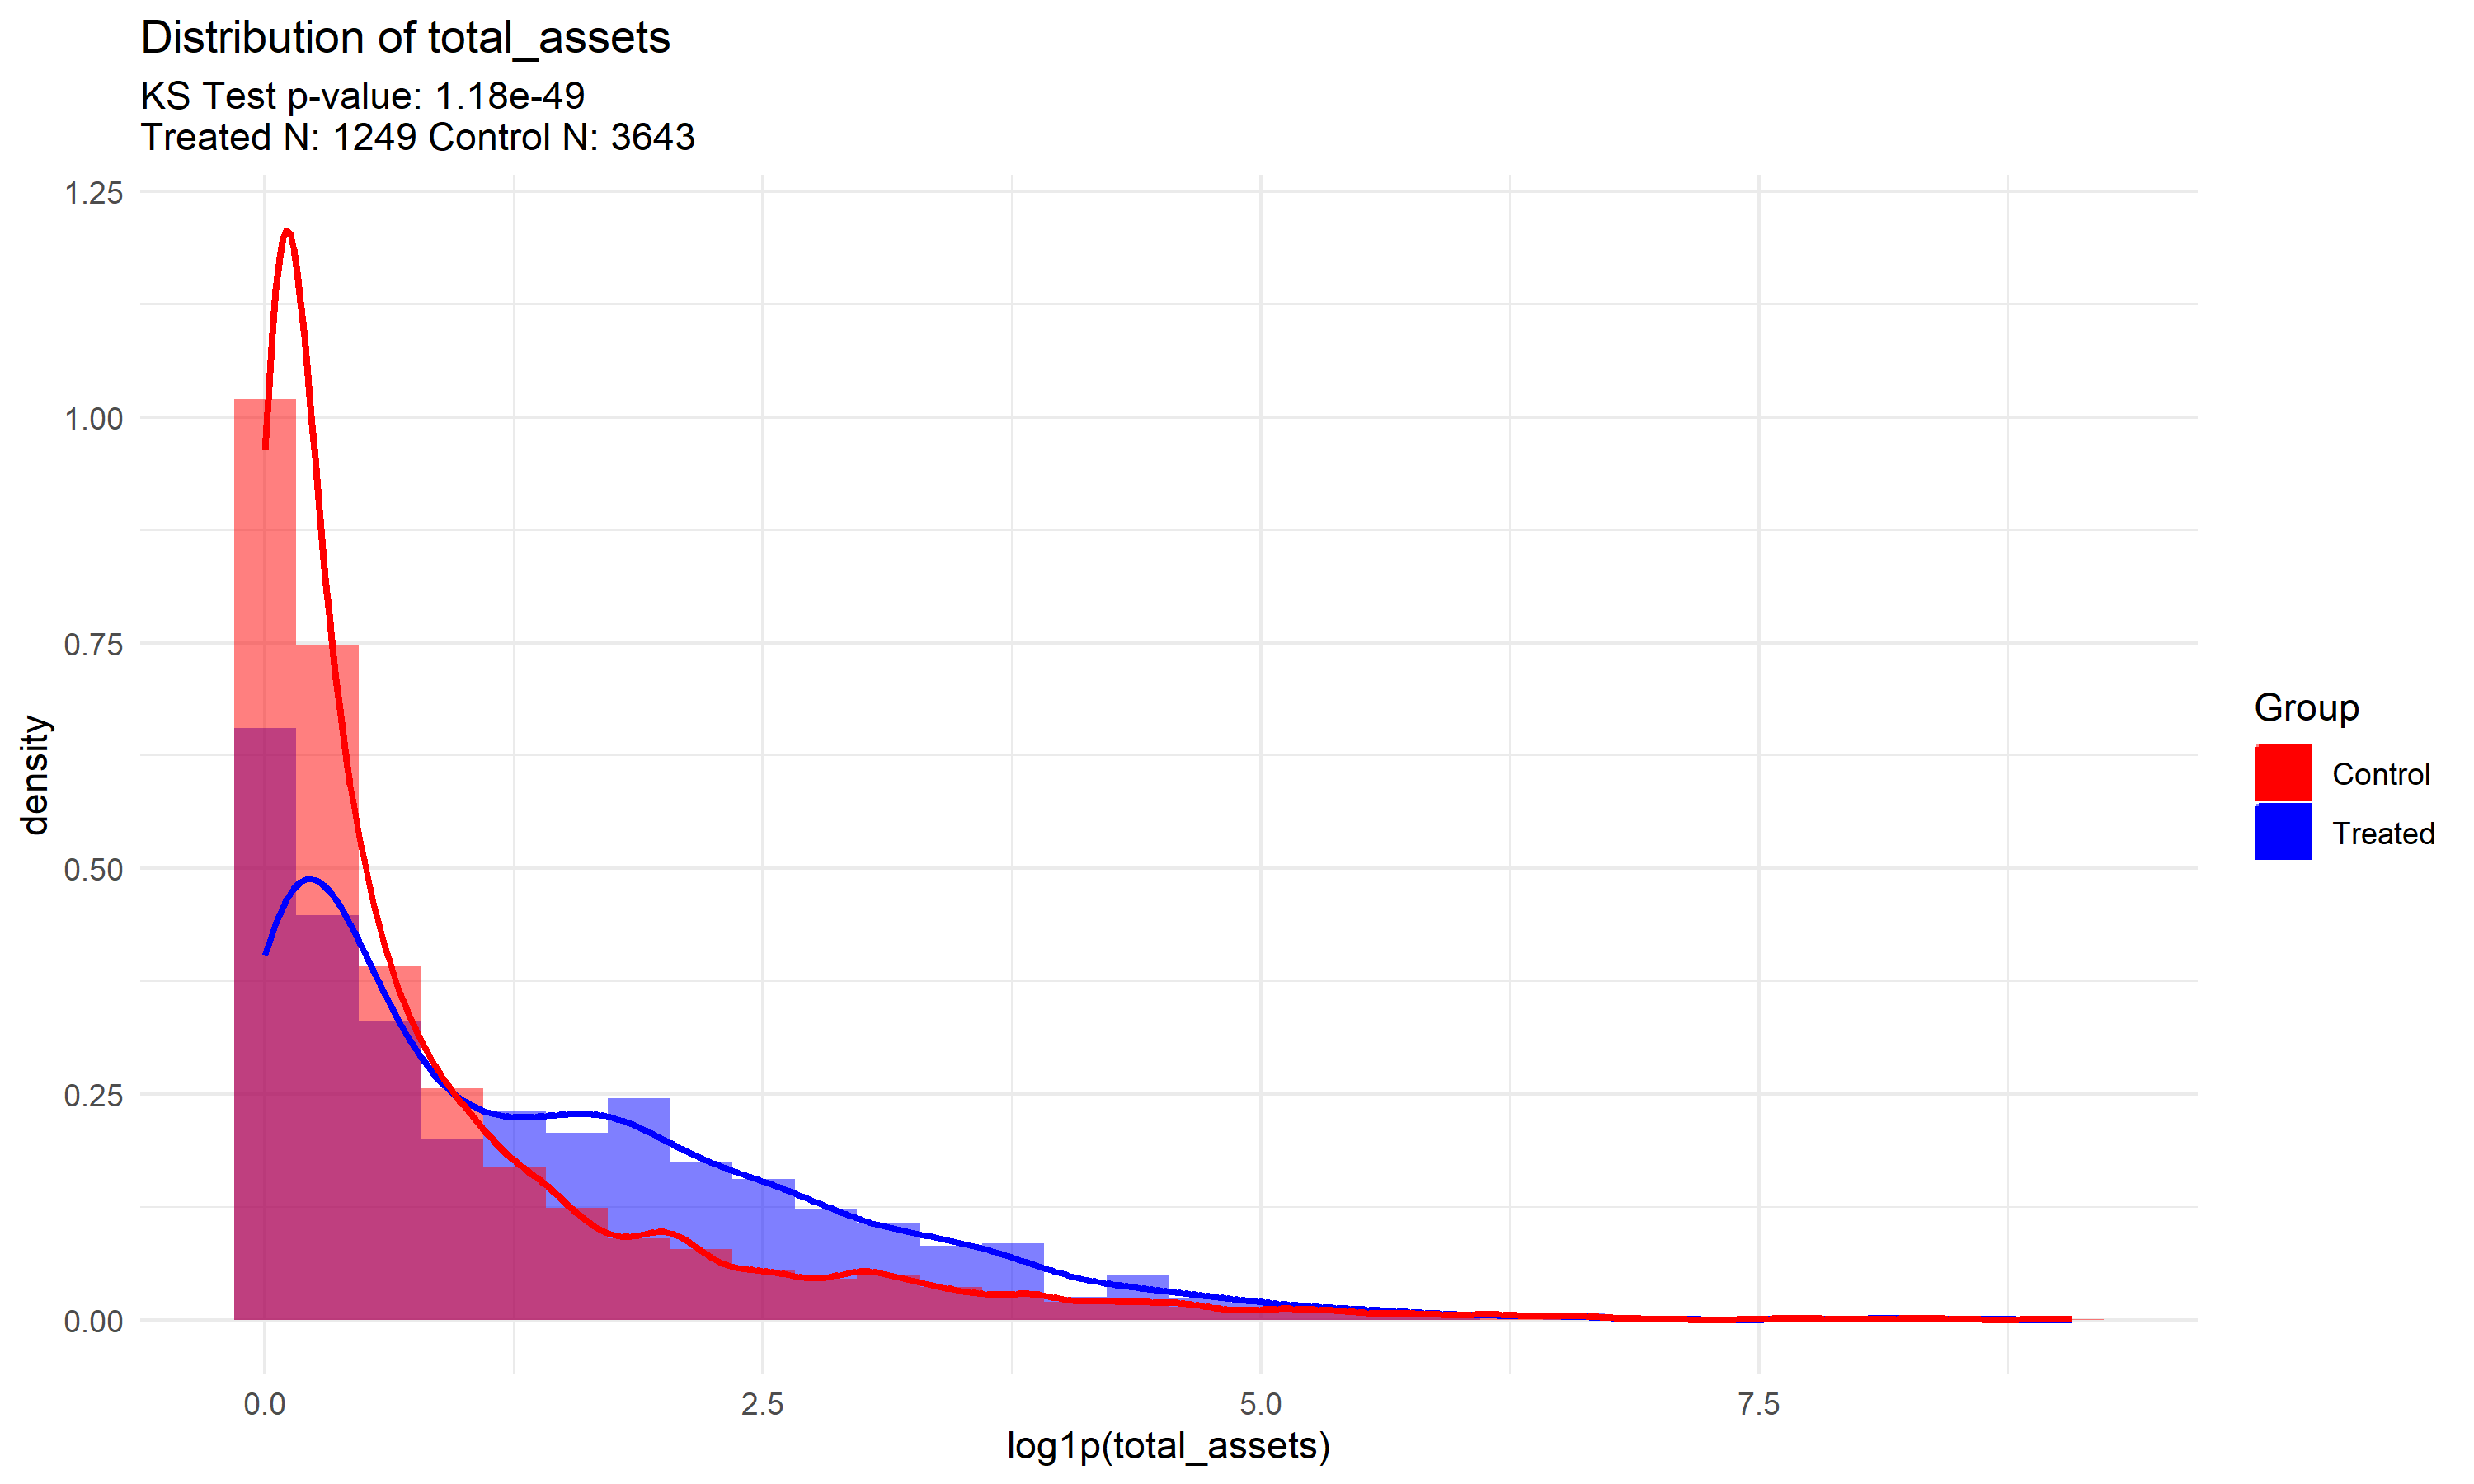
\includegraphics[width=\linewidth]{../Output/distrib_compare_total_assets_allcountries.png}
                \caption{Total Assets}

            \end{subfigure}
            \hfill
            \begin{subfigure}[b]{0.45\textwidth}
                \centering
                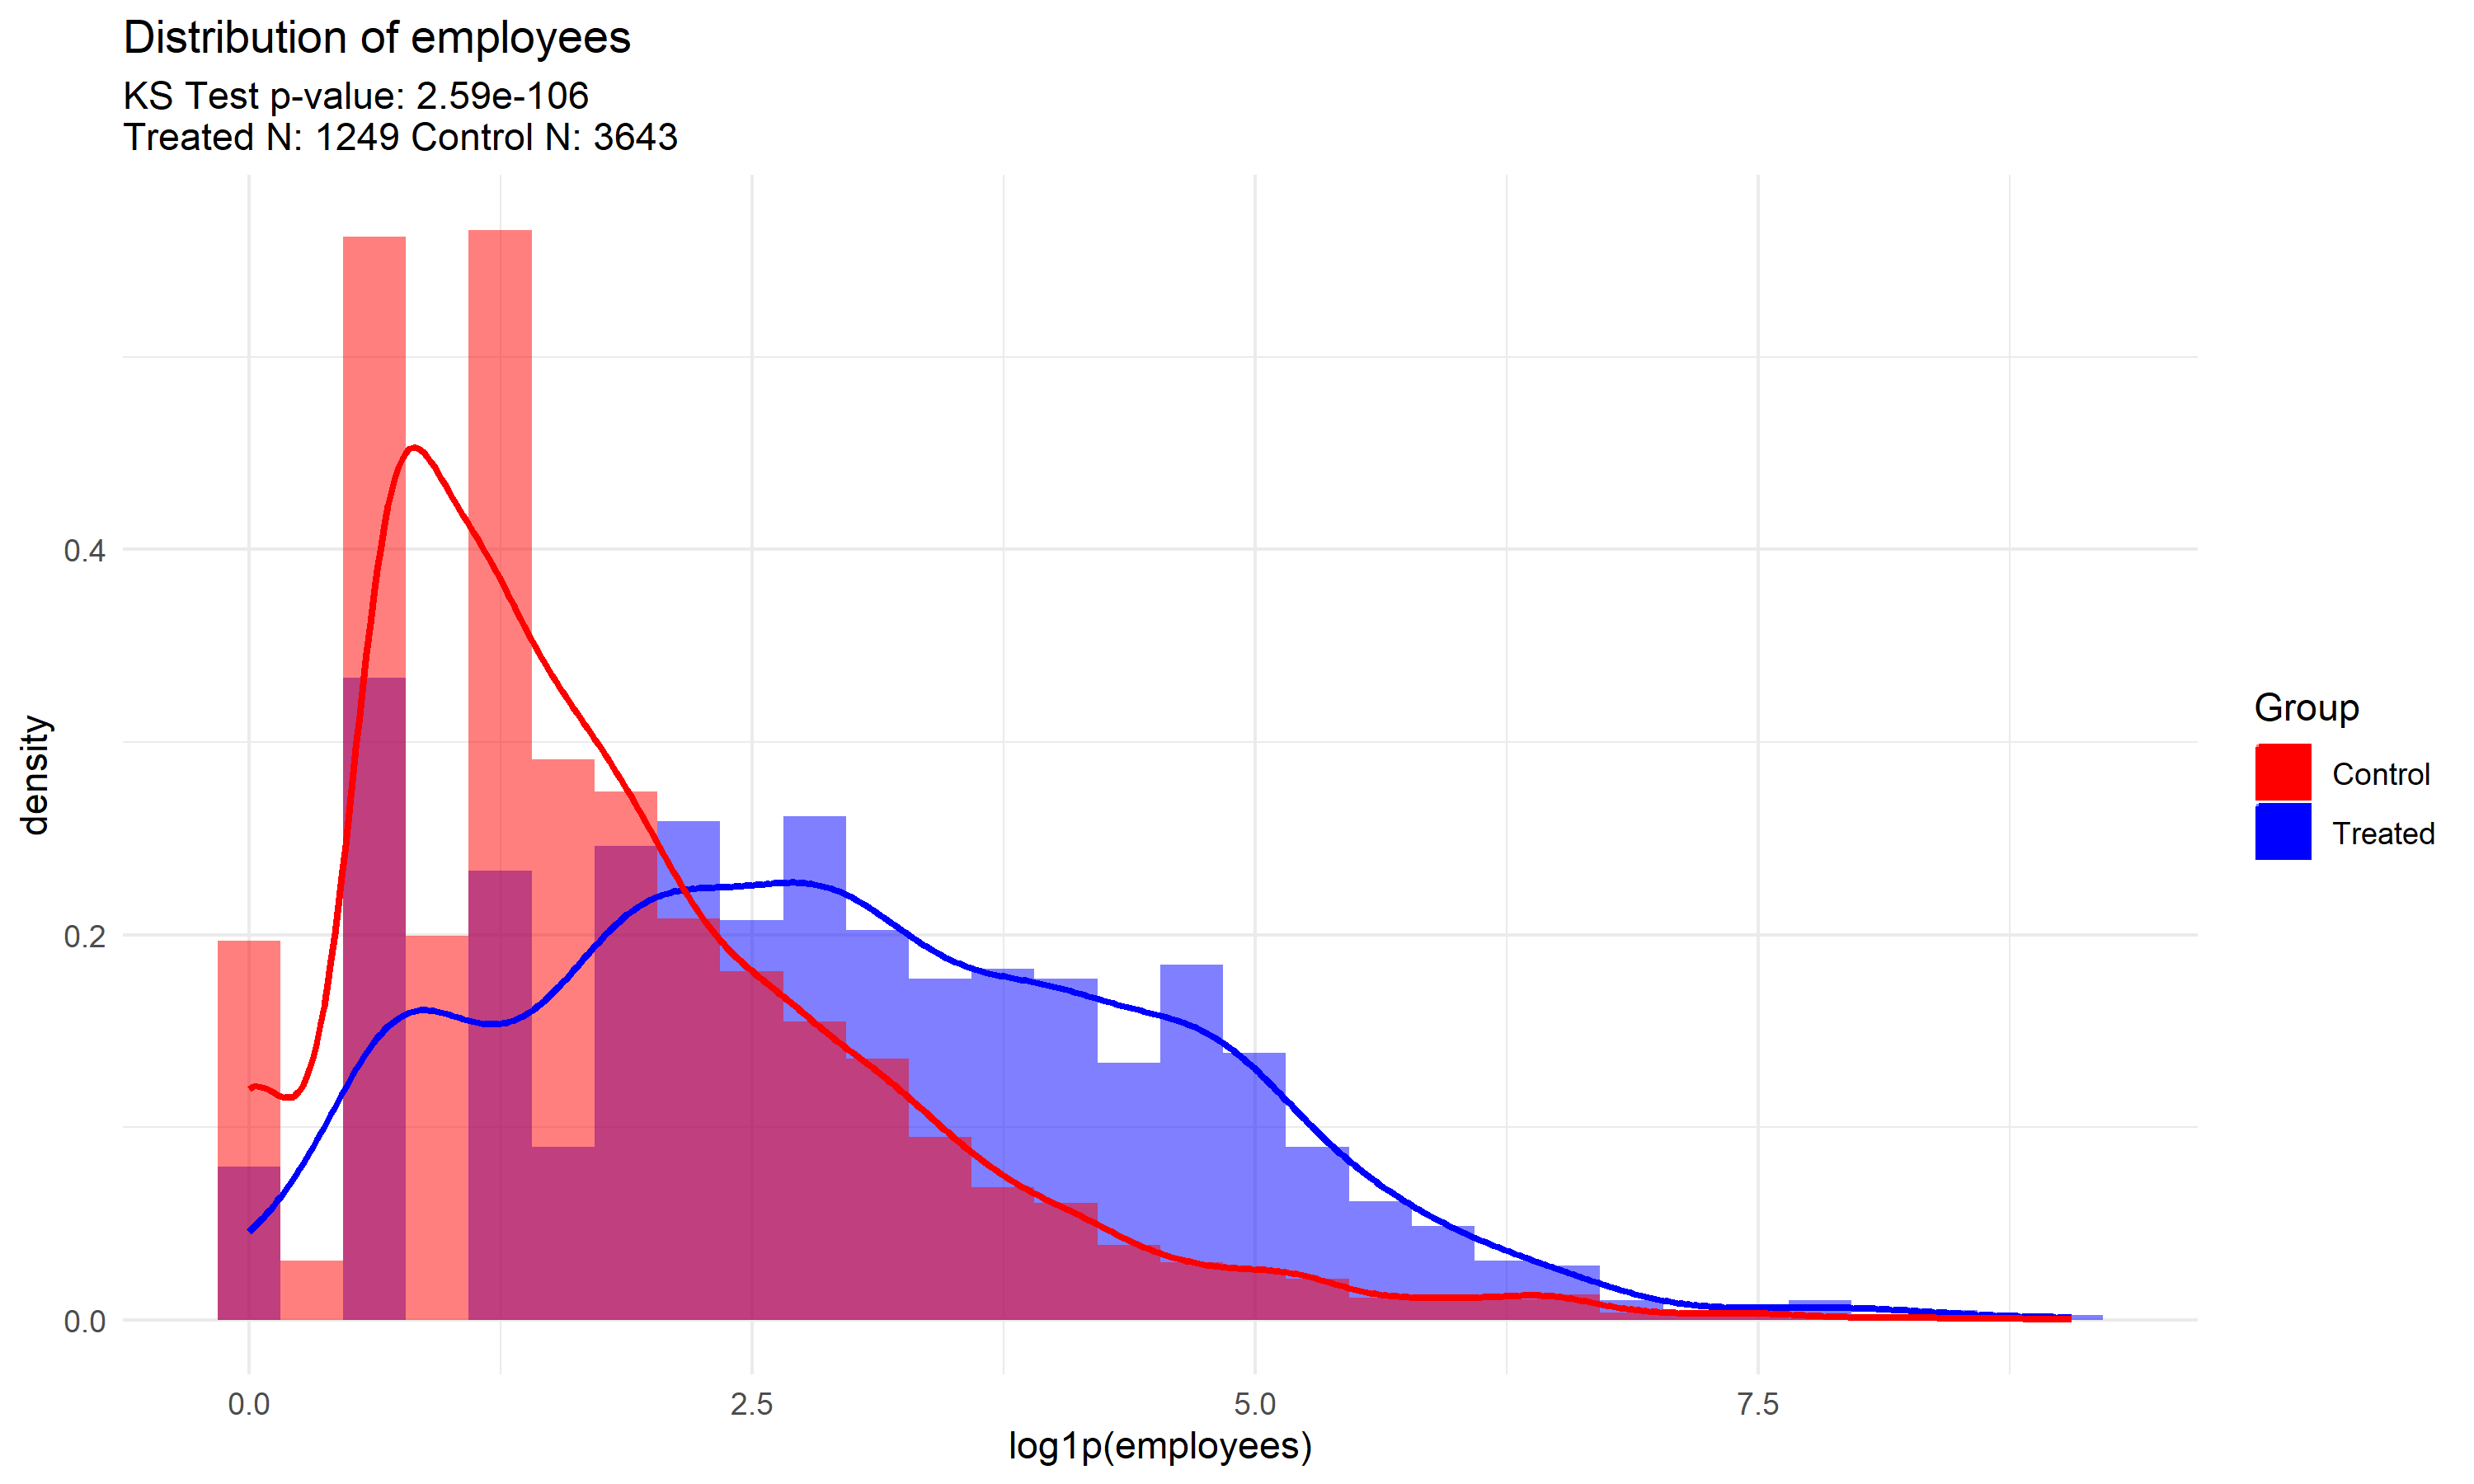
\includegraphics[width=\linewidth]{../Output/distrib_compare_employees_allcountries.png}
                \caption{Employees}
                \label{fig:employees}
            \end{subfigure}
            \vspace{0.5cm}
            \begin{subfigure}[b]{0.45\textwidth}
                \centering
                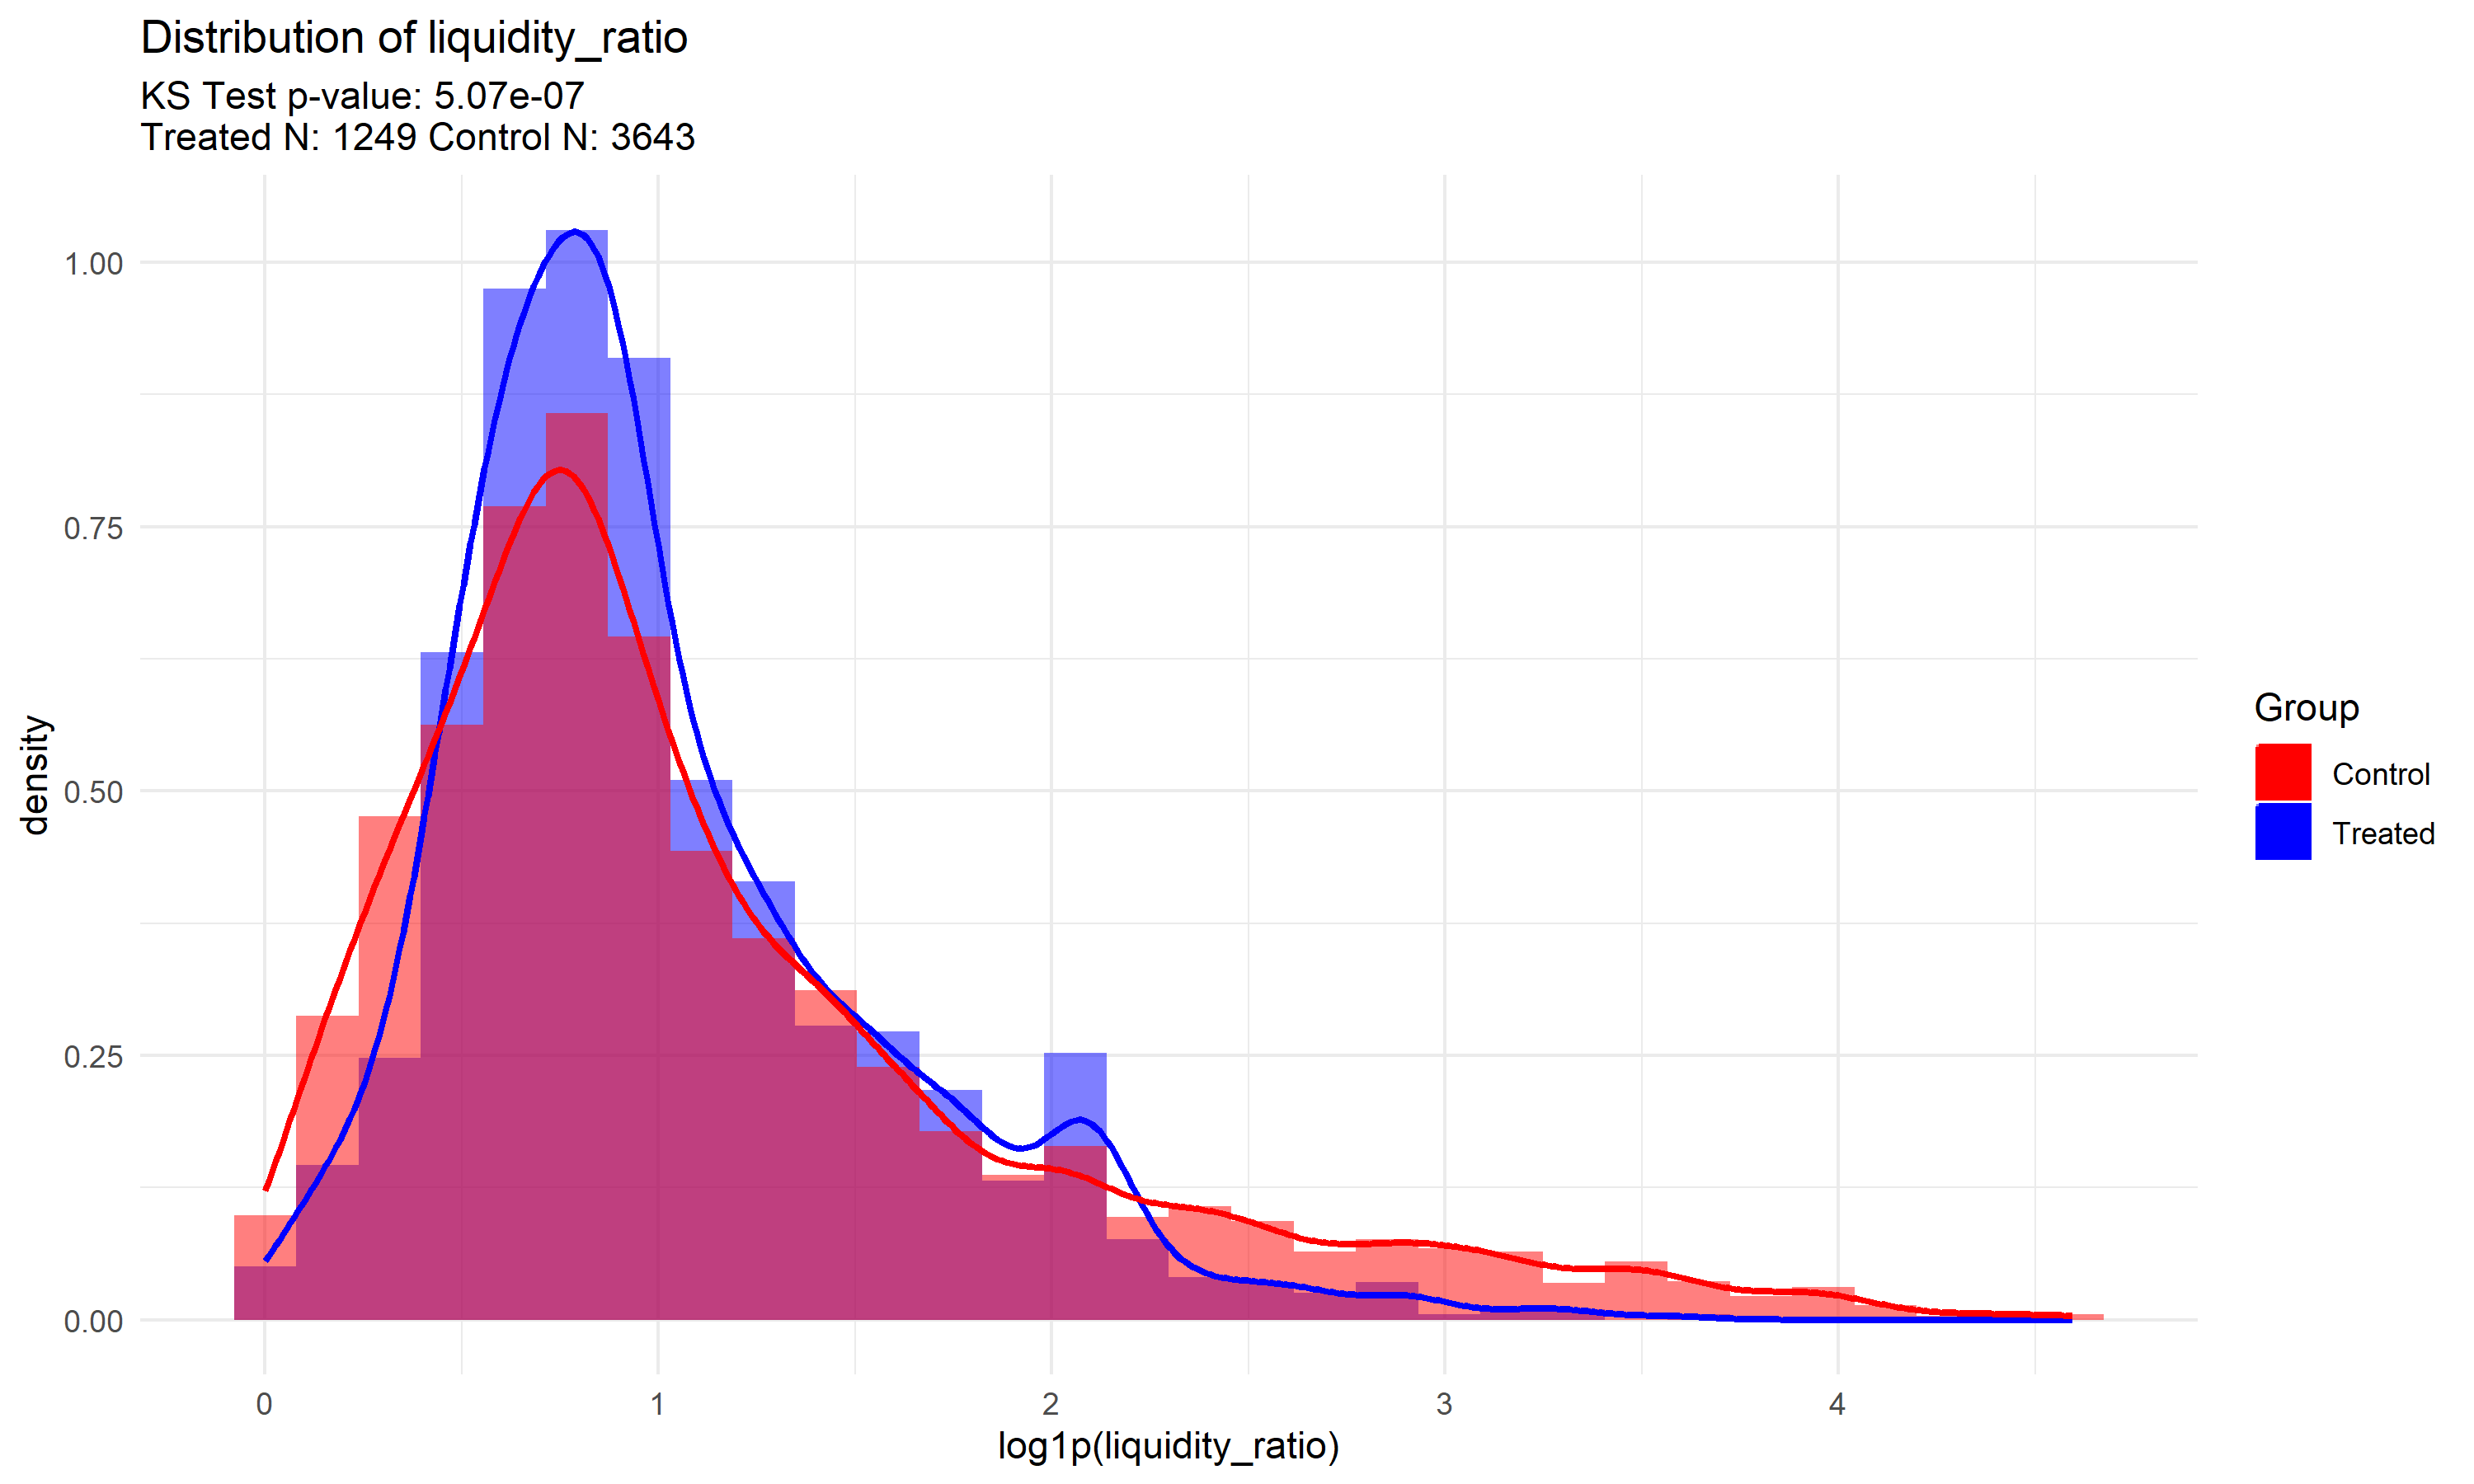
\includegraphics[width=\linewidth]{../Output/distrib_compare_liquidity_ratio_allcountries.png}
                \caption{Liquidity Ratio}

            \end{subfigure}
            \hfill
            \begin{subfigure}[b]{0.45\textwidth}
                \centering
                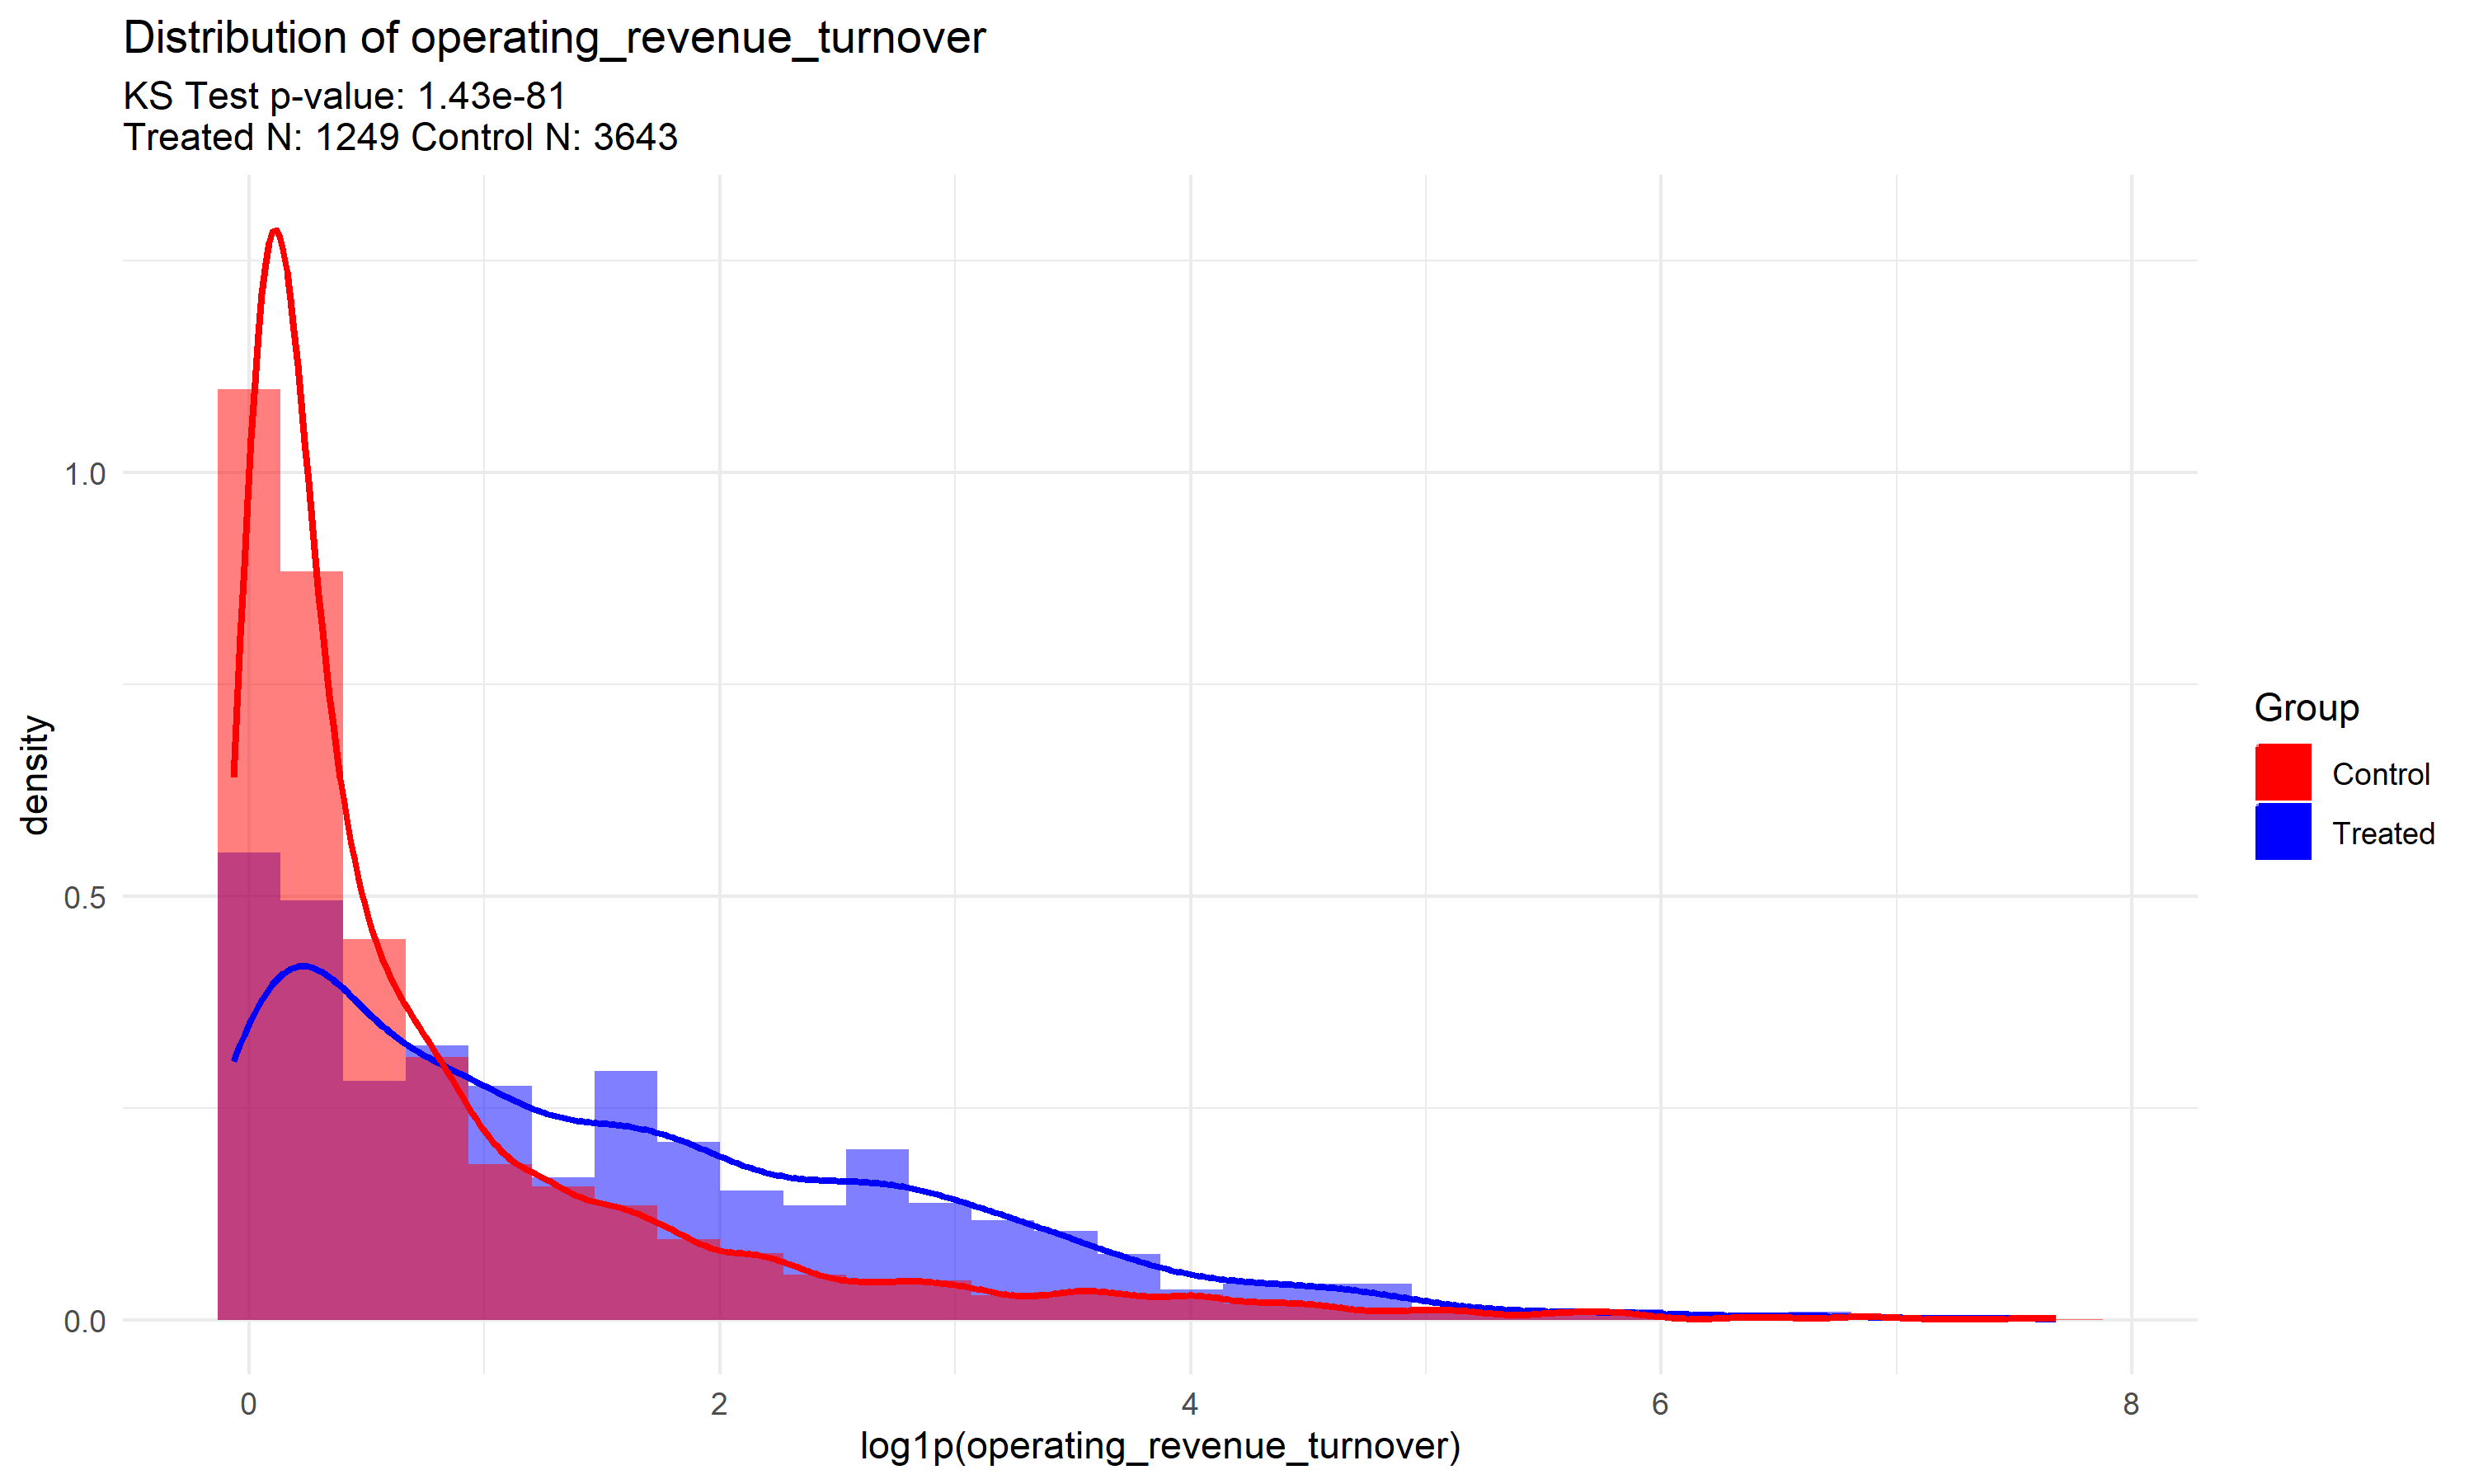
\includegraphics[width=\linewidth]{../Output/distrib_compare_operating_revenue_turnover_allcountries.png}
                \caption{Turnover}

            \end{subfigure}
            \vspace{0.5cm}
        \end{figure}
\end{frame}


\begin{frame}{Treated vs Control - Distributions Compared Part 2}
    \begin{figure}[ht]
        \centering
        \begin{subfigure}[b]{0.45\textwidth}
            
            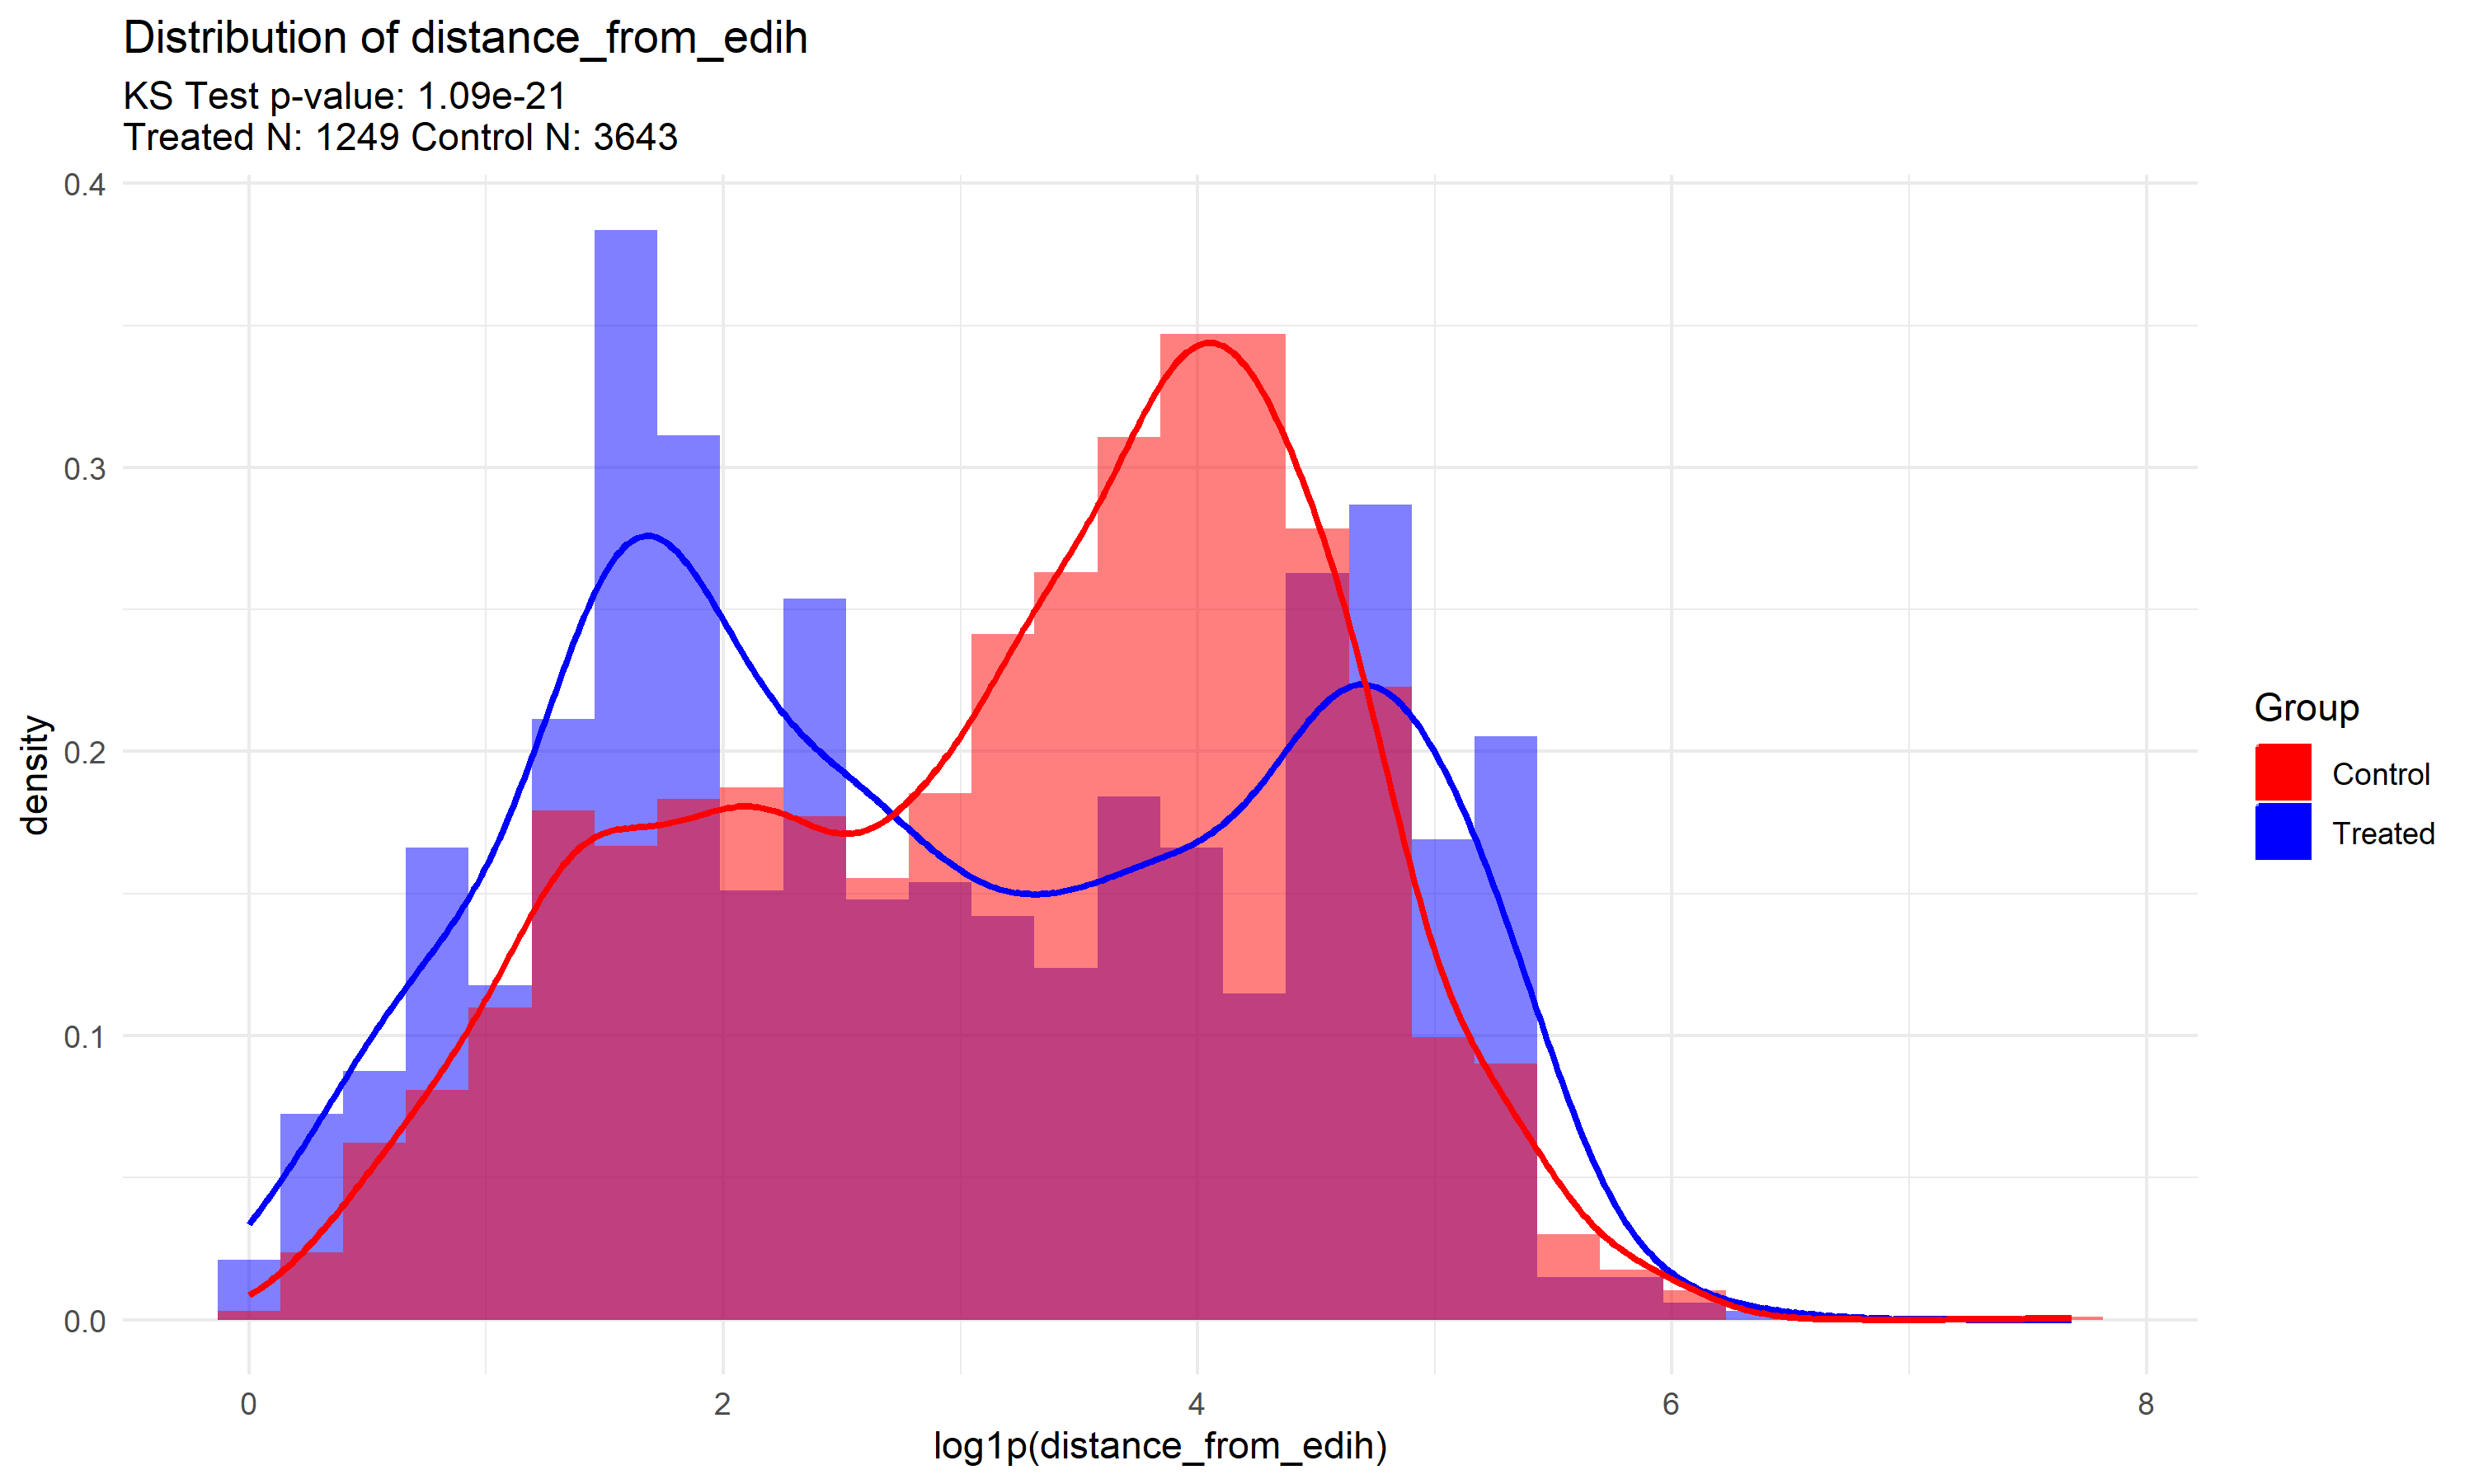
\includegraphics[width=\linewidth]{../Output/distrib_compare_distance_from_edih_allcountries.png}
            \caption{Distance from EDIH}

        \end{subfigure}
        \hfill
        \begin{subfigure}[b]{0.45\textwidth}
            \centering
            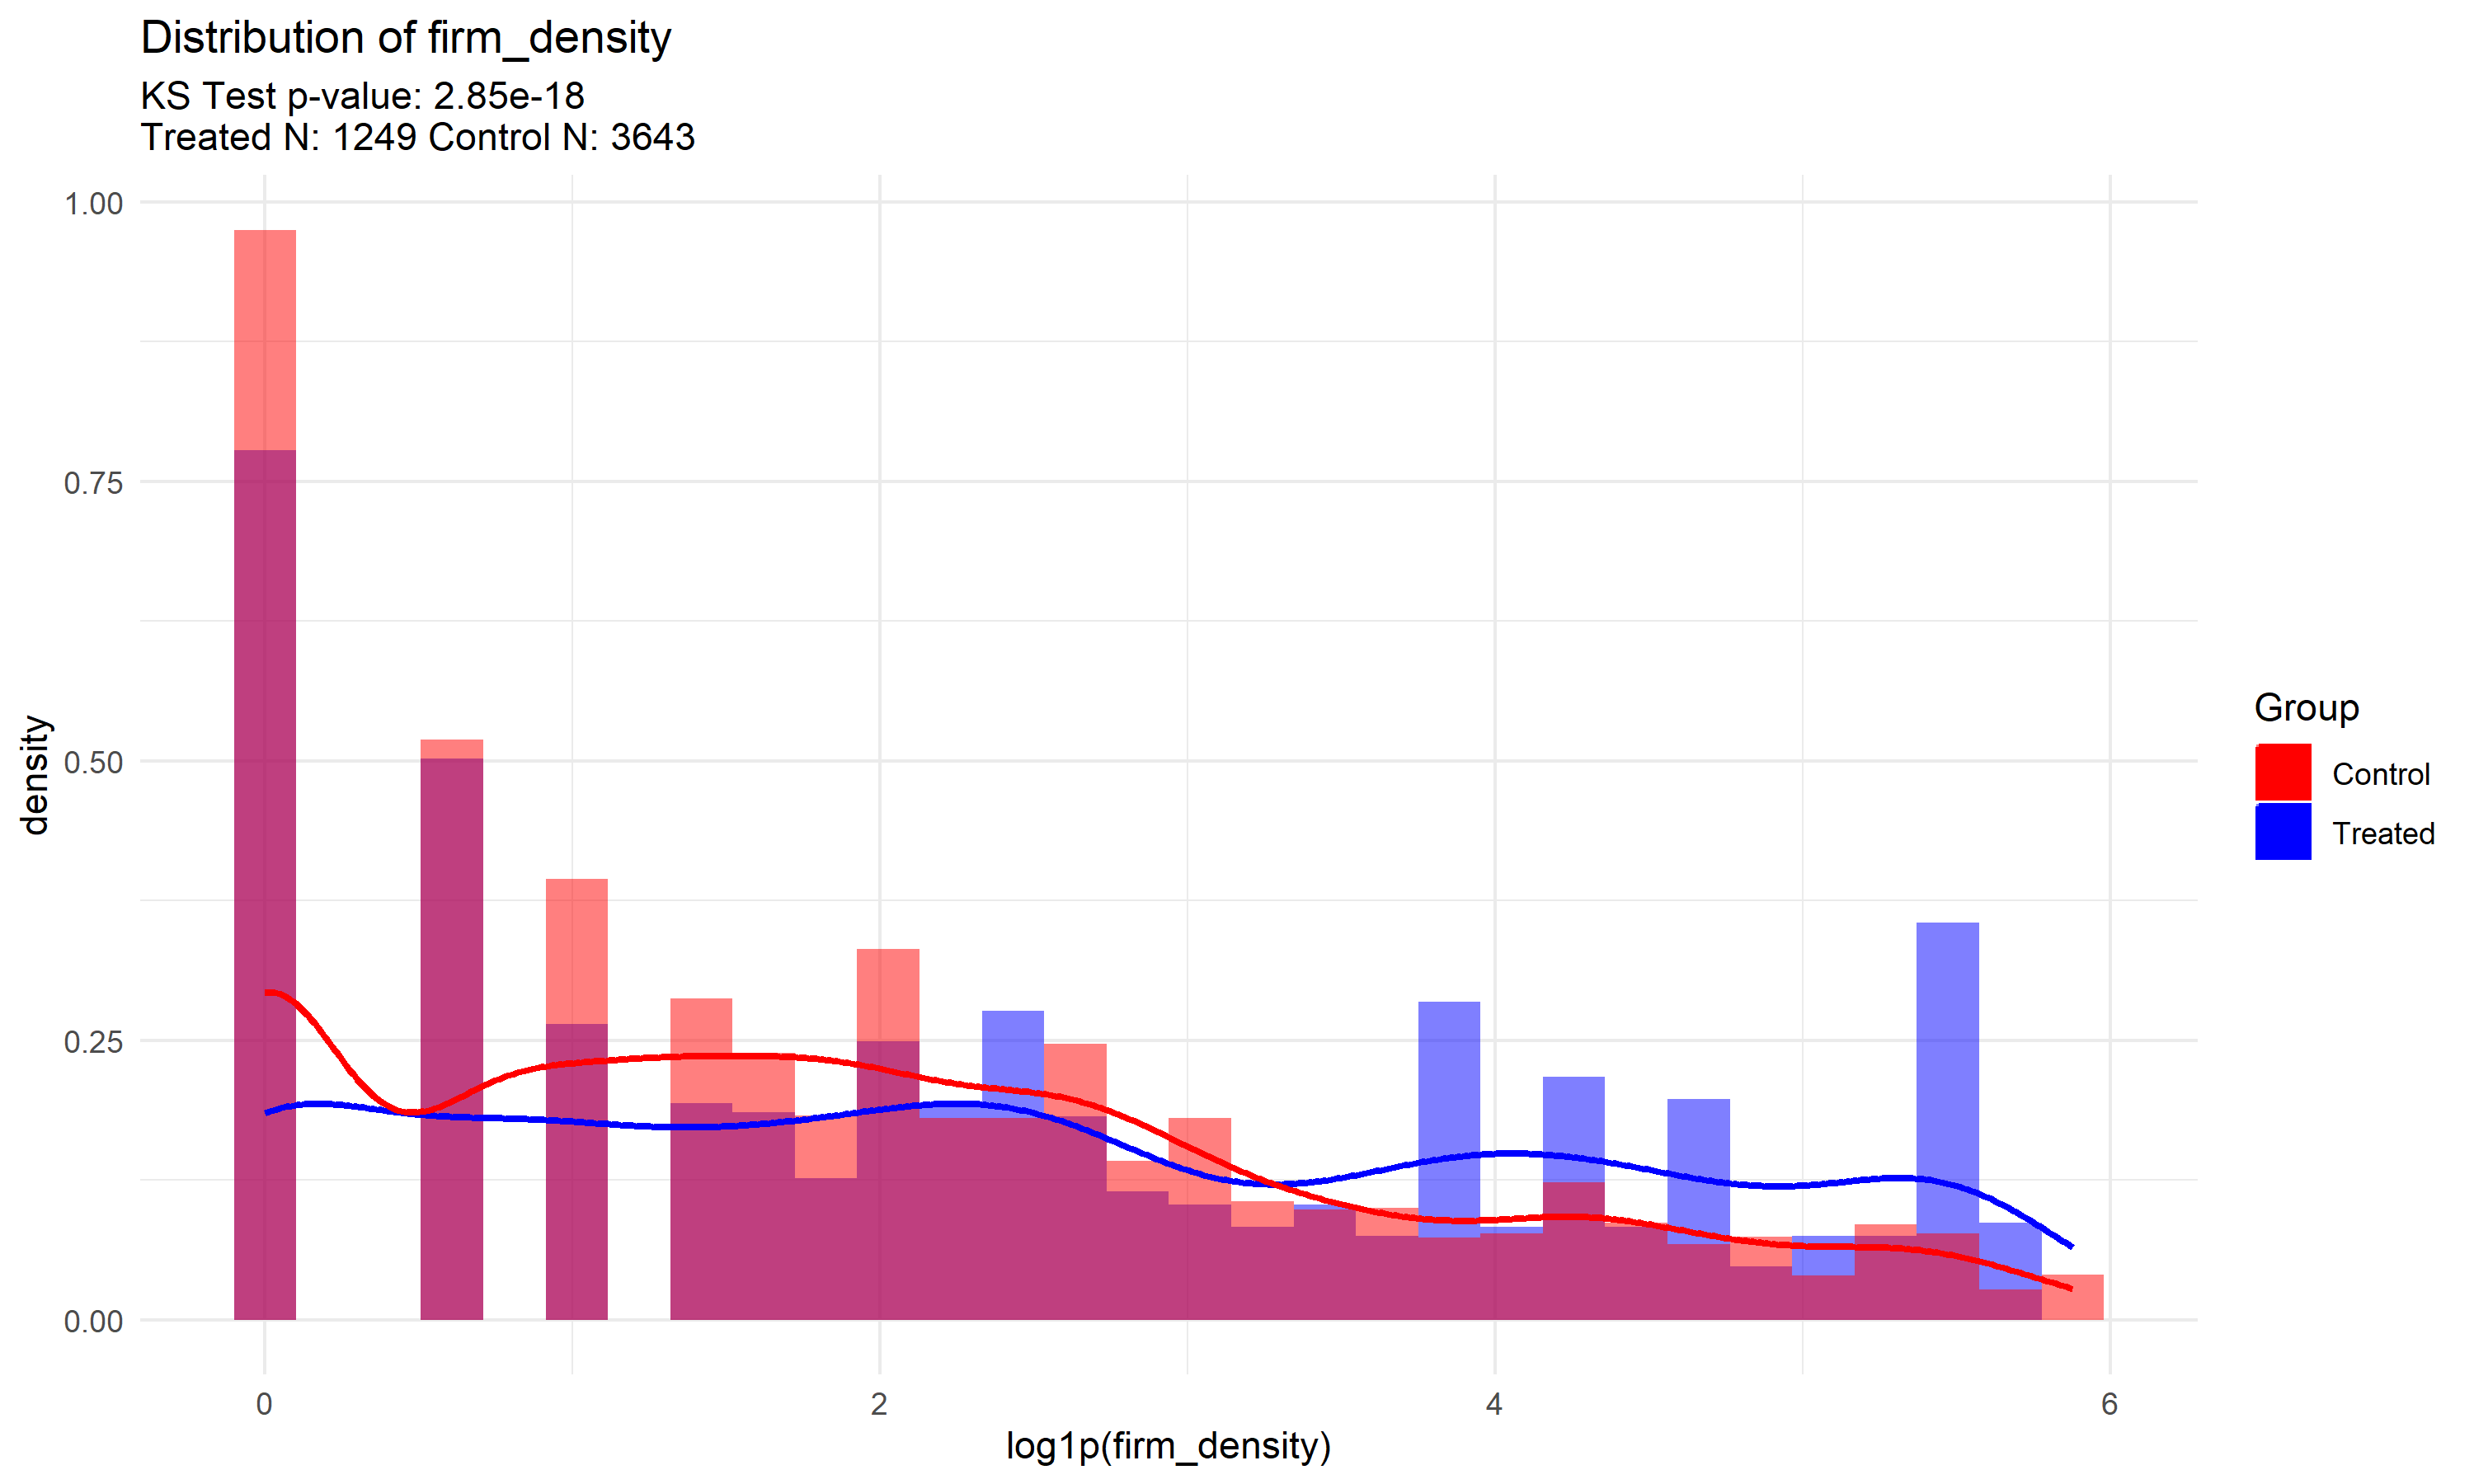
\includegraphics[width=\linewidth]{../Output/distrib_compare_firm_density_allcountries.png}
            \caption{Firm Density}

        \end{subfigure}
        \vspace{0.5cm}
        \begin{subfigure}[b]{0.45\textwidth}
            \centering
            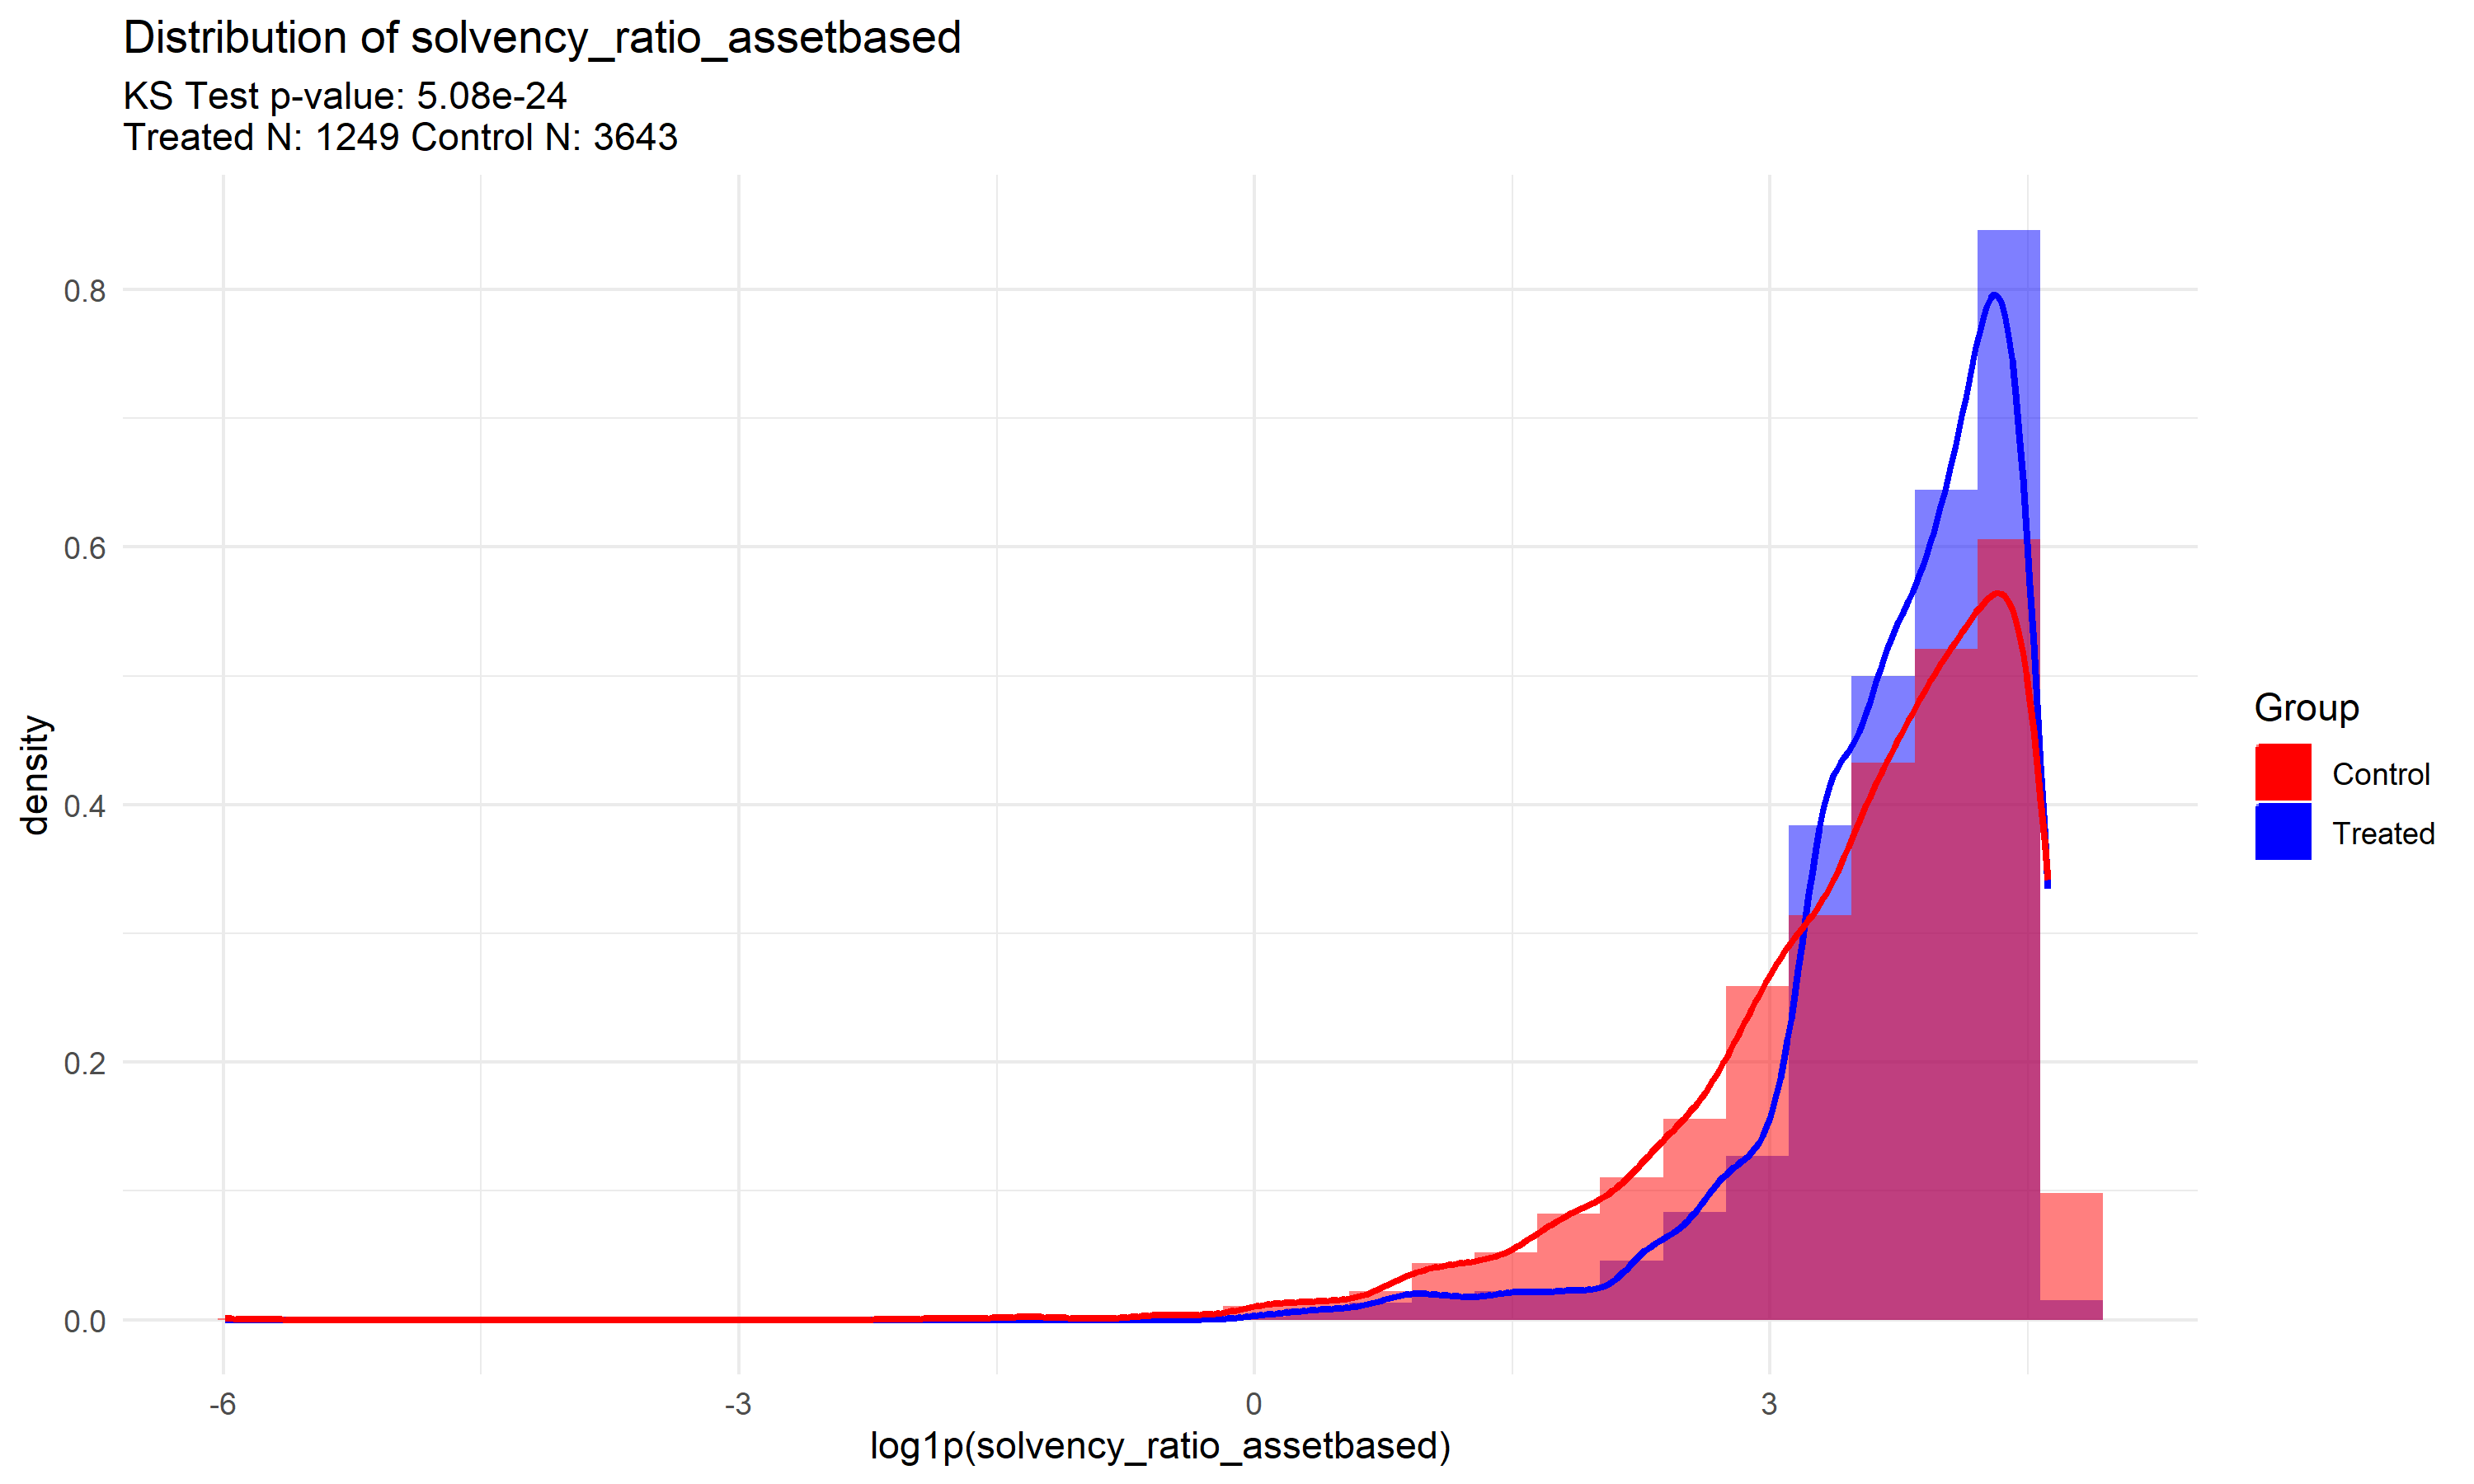
\includegraphics[width=\linewidth]{../Output/distrib_compare_solvency_ratio_assetbased_allcountries.png}
            \caption{Solvency Ratio}
        \end{subfigure}
    \end{figure}
\end{frame}



\begin{frame}{Firm Density - Definition}
    \hypertarget{firm_density_slide}{}
        \begin{itemize}
            \item \textbf{Definition:} Firm density is defined as the number of firms within a 5 km radius of a given firm, excluding EDIHs.
        \end{itemize}
        \centering
        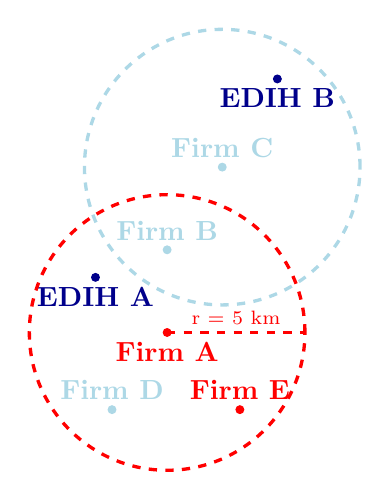
\begin{tikzpicture}[scale=0.7] % Scale everything by 0.7
                % Draw a horizontal segmented line to represent the radius
                \draw[red, thick, dashed] (0,0) -- (2.5,0) node[midway, above=-1pt, font=\scriptsize] {r = 5 km};    
                % Draw firms as dots
                \filldraw[red] (0,0) circle (2pt) node[anchor=north] {\textbf{Firm A}};
                \filldraw[lightblue] (0,1.5) circle (2pt) node[anchor=south] {\textbf{Firm B}};
                \filldraw[lightblue] (1,3) circle (2pt) node[anchor=south] {\textbf{Firm C}};
                \filldraw[darkblue] (-1.3,1) circle (2pt) node[anchor=north] {\textbf{EDIH A}};
                \filldraw[darkblue] (2,4.6) circle (2pt) node[anchor=north] {\textbf{EDIH B}};
                \filldraw[lightblue] (-1,-1.4) circle (2pt) node[anchor=south] {\textbf{Firm D}};
                \filldraw[red] (1.32,-1.4) circle (2pt) node[anchor=south] {\textbf{Firm E}};
                
                % Draw a circle around the firms to represent density
                \draw[red, very thick, dashed] (0,0) circle (2.5cm);
        
                \draw[lightblue, very thick, dashed] (1,3) circle (2.5cm);
        \end{tikzpicture}
\end{frame}


\begin{frame}{Regression Results - Sectoral Subsamples}
    
% Table created by stargazer v.5.2.3 by Marek Hlavac, Social Policy Institute. E-mail: marek.hlavac at gmail.com
% Date and time: dom, gen 19, 2025 - 23:36:23
\begin{table}[!htbp] \centering 
  \tiny
  \renewcommand{\arraystretch}{1} 
    \label{} 
\begin{tabular}{@{\extracolsep{5pt}}lccc} 
\\[-1.8ex]\hline 
\hline \\[-1.8ex] 
 & \multicolumn{3}{c}{\textit{Dependent variable: Treated}} \\ 
\cline{2-4} 
\\[-1.8ex] & \multicolumn{3}{c}{} \\ 
 & Manufacturing & Services & Other \\ 
\hline \\[-1.8ex] 
 Dist. from EDIH & $-$0.004$^{***}$ & $-$0.001$^{**}$ & $-$0.001 \\ 
  & (0.001) & (0.001) & (0.001) \\ 

 Firm Density & $-$0.004$^{**}$ & 0.002$^{***}$ & 0.001 \\ 
  & (0.002) & (0.001) & (0.002) \\ 

 High Tech & 0.603 & 1.769$^{***}$ &  \\ 
  & (0.698) & (0.255) &  \\ 
 
 Medium Tech & 0.605 &  & 0.784$^{**}$ \\ 
  & (0.655) &  & (0.383) \\ 

 Medium-High Tech & 1.333$^{**}$ & 1.669$^{***}$ &  \\ 
  & (0.644) & (0.106) &  \\ 
 
 Medium-Low Tech & 0.781 & 0.554$^{***}$ & 0.733 \\ 
  & (0.640) & (0.080) & (0.615) \\ 

 Turnover & $-$0.003$^{***}$ & 0.001$^{**}$ & $-$0.004$^{***}$ \\ 
  & (0.001) & (0.001) & (0.001) \\ 

 Employees & 1.664$^{***}$ & 0.616$^{***}$ & 9.114$^{***}$ \\ 
  & (0.484) & (0.170) & (1.615) \\ 

 Liquidity Ratio & $-$0.118$^{***}$ & $-$0.086$^{***}$ & $-$0.100$^{***}$ \\ 
  & (0.023) & (0.010) & (0.035) \\ 

 Solvency Ratio & 0.015$^{***}$ & 0.010$^{***}$ & 0.009$^{***}$ \\ 
  & (0.003) & (0.001) & (0.003) \\ 

 

\hline \\[-1.8ex] 
Observations & 842 & 3,084 & 938 \\ 

\hline 
\hline \\[-1.8ex] 
\textit{Note:}  & \multicolumn{3}{r}{$^{*}$p$<$0.1; $^{**}$p$<$0.05; $^{***}$p$<$0.01} \\ 
\end{tabular} 
\end{table} 
\end{frame}








\begin{frame}{References}
    \printbibliography
\end{frame}


\end{document}